% ****************************************************************************************** % Dissertation template and document class for Princeton University
% Author  : Jeffrey Scott Dwoskin <jdwoskin@princeton.edu>
% Adapted from: http://www.math.princeton.edu/graduate/tex/puthesis.html
% ****************************************************************************************** %


%%% For print copies
%% set 'singlespace' option to set entire thesis to single space, and define "\printmode" to remove all hyperlinks for printed copies of the thesis. Delete all output files before changing this mode -- it will turn hyperref package on and off
% \documentclass[12pt,lot, lof, singlespace]{puthesis}
% \newcommand{\printmode}{}

%%% For the electronic copy, use doublespacing, define "\proquestmode" to use outlined links, instead of colored links. 
\documentclass[12pt,lot, lof]{puthesis}
% \newcommand{\proquestmode}{}
% I prefer proquestmode to be off for electronic copies for normal use, since the colored links are less distracting. However when printed in black and white, the colored links are difficult to read. 

%%% For early drafts without some of the frontmatter
% Also see the "ifodd" command below to disable more frontmatter
%\documentclass[12pt]{puthesis}

%%%%%%%%%%%%%%%%%%%%%%%%%%%%%%%%%%%%%%%%%%%%%%%%%%%%%%%%%%%%%\
%%%% Author & title page info

\title{Manifold Learning for States and Parameters}

\submitted{September 2017}  % degree conferral date (January, April, June, September, or November)
\copyrightyear{2017}  % year in which the copyright is secured by publication of the dissertation.
\author{Alexander Holiday}
\adviser{Professor Ioannis G. Kevrekidis}  %replace with the full name of your adviser
%\departmentprefix{Program in}  % defaults to "Department of", but programs need to change this.
\department{Chemical and Biological Engineering}

%%%%%%%%%%%%%%%%%%%%%%%%%%%%%%%%%%%%%%%%%%%%%%%%%%%%%%%%%%%%%\
%%%% Tweak float placements
% From: http://mintaka.sdsu.edu/GF/bibliog/latex/floats.html "Controlling LaTeX Floats"
% and based on: http://www.tex.ac.uk/cgi-bin/texfaq2html?label=floats
% LaTeX defaults listed at: http://people.cs.uu.nl/piet/floats/node1.html

% Alter some LaTeX defaults for better treatment of figures:
    % See p.105 of "TeX Unbound" for suggested values.
    % See pp. 199-200 of Lamport's "LaTeX" book for details.
    %   General parameters, for ALL pages:
    \renewcommand{\topfraction}{0.85}	% max fraction of floats at top
    \renewcommand{\bottomfraction}{0.6}	% max fraction of floats at bottom
    %   Parameters for TEXT pages (not float pages):
    \setcounter{topnumber}{2}
    \setcounter{bottomnumber}{2}
    \setcounter{totalnumber}{4}     % 2 may work better
    \setcounter{dbltopnumber}{2}    % for 2-column pages
    \renewcommand{\dbltopfraction}{0.66}	% fit big float above 2-col. text
    \renewcommand{\textfraction}{0.15}	% allow minimal text w. figs
    %   Parameters for FLOAT pages (not text pages):
    \renewcommand{\floatpagefraction}{0.66}	% require fuller float pages
	% N.B.: floatpagefraction MUST be less than topfraction !!
    \renewcommand{\dblfloatpagefraction}{0.66}	% require fuller float pages

% The documentclass already sets parameters to make a high penalty for widows and orphans. 

%%%%%%%%%%%%%%%%%%%%%%%%%%%%%%%%%%%%%%%%%%%%%%%%%%%%%%%%%%%%%\
%%%% Use packages

%\usepackage{amsfonts}

%%% For figures
% \usepackage{graphicx}
\usepackage[draft]{graphicx}
\graphicspath{
  {./ch-graphs/figs/}
  {./ch-params/figs/}}
%\usepackage{subfig,rotate}
\usepackage{subcaption}

\DeclareCaptionSubType[Alph]{figure}
\captionsetup[subfigure]{labelformat=simple, font=sf}

% for chemistry arrows
\usepackage{chemarr}

% for nice arrays
\usepackage{blkarray}

\usepackage{epstopdf}

%%% for comments
\usepackage{verbatim}

%%% For tables
\usepackage{multirow}
% Longtable lets you have tables that span multiple pages.
\usepackage{longtable}

% Booktabs produces far nicer tables than the standard LaTeX tables.
%   see: http://en.wikibooks.org/wiki/LaTeX/Tables
\usepackage{booktabs}

%set parameters for longtable:
% default caption width is 4in for longtable, but wider for normal tables
\setlength{\LTcapwidth}{\textwidth}


%% For math
\usepackage{amsmath, amsfonts, amssymb}
\DeclareMathOperator*{\argmin}{arg\,min}

\usepackage[sort]{natbib}

%% notation
\def \data {\mathbf{y}}
\def \dataone {y}
\def \measfn {\mathbf{f}}
\def \ndata {m}
\def \lowdim {d}
\def \lowdimslow { {d_1} }
\def \highdim {n}
\def \rotdim {d_{rot}}
\def \dmeps {\sigma_{kernel}}
\def \manifold {\mathcal{M}_\lowdim}

\def \chap {Chapter}
\def \fig {Figure}
\def \sec {Section}
\def \app {Appendix}
\def \tab {Table}

%%%%%%%%%%%%%%%%%%%%%%%%%%%%%%%%%%%%%%%%%%%%%%%%%%%%%%%%%%
%%% Printed vs. online formatting
\ifdefined\printmode

% Printed copy
% url package understands urls (with proper line-breaks) without hyperlinking them
\usepackage{url}
\usepackage[hidelinks]{hyperref}
%\usepackage[top=1in,left=1.5in,bottom=1in,right=1in,footskip=0.25in]{geometry}

\else

\ifdefined\proquestmode
%ProQuest copy -- http://www.princeton.edu/~mudd/thesis/Submissionguide.pdf

% ProQuest requires a double spaced version (set previously). They will take an electronic copy, so we want links in the pdf, but also copies may be printed or made into microfilm in black and white, so we want outlined links instead of colored links.
\usepackage{hyperref}
\hypersetup{bookmarksnumbered}

%\usepackage[top=1in,left=1in,bottom=1in,right=1in,footskip=0.25in]{geometry}
\oddsidemargin 0in   %{.4375in}
\textwidth 6.5in

% copy the already-set title and author to use in the pdf properties
\makeatletter
\hypersetup{pdftitle=\@title,pdfauthor=\@author}
\makeatother

\else
% Online copy

% adds internal linked references, pdf bookmarks, etc

% turn all references and citations into hyperlinks:
%  -- not for printed copies
% -- automatically includes url package
% options:
%   colorlinks makes links by coloring the text instead of putting a rectangle around the text.
\usepackage{hyperref}
\hypersetup{colorlinks,bookmarksnumbered}

% copy the already-set title and author to use in the pdf properties
\makeatletter
\hypersetup{pdftitle=\@title,pdfauthor=\@author}
\makeatother

% make the page number rather than the text be the link for ToC entries
%\hypersetup{linktocpage}
\fi % proquest or online formatting
\fi % printed or online formatting


%%%%%%%%%%%%%%%%%%%%%%%%%%%%%%%%%%%%%%%%%%%%%%%%%%%%%%%%%%%%%\
%%%% Define commands

% Define any custom commands that you want to use.
% For example, highlight notes for future edits to the thesis
%\newcommand{\todo}[1]{\textbf{\emph{TODO:}#1}}

% minus sign be better
\newcommand{\minus}{\scalebox{0.75}[1.0]{$-$}}

% create an environment that will indent text
% see: http://latex.computersci.org/Reference/ListEnvironments
% 	\raggedright makes them left aligned instead of justified
\newenvironment{indenttext}{
    \begin{list}{}{ \itemsep 0in \itemindent 0in
    \labelsep 0in \labelwidth 0in
    \listparindent 0in
    \topsep 0in \partopsep 0in \parskip 0in \parsep 0in
    \leftmargin 1em \rightmargin 0in
    \raggedright
    }
    \item
  }
  {\end{list}}

% another environment that's an indented list, with no spaces between items -- if we want multiple items/lines. Useful in tables. Use \item inside the environment.
% 	\raggedright makes them left aligned instead of justified
\newenvironment{indentlist}{
    \begin{list}{}{ \itemsep 0in \itemindent 0in
    \labelsep 0in \labelwidth 0in
    \listparindent 0in
    \topsep 0in \partopsep 0in \parskip 0in \parsep 0in
    \leftmargin 1em \rightmargin 0in
    \raggedright
    }

  }
  {\end{list}}




%%%%%%%%%%%%%%%%%%%%%%%%%%%%%%%%%%%%%%%%%%%%%%%%%%%%%%%%%%%%%\
%%%% Front-matter

% For early drafts, you may want to disable some of the frontmatter. Simply change this to "\ifodd 1" to do so.
\ifodd 0
% front-matter disabled while writing chapters
\renewcommand{\maketitlepage}{}
\renewcommand*{\makecopyrightpage}{}
\renewcommand*{\makeabstract}{}

% you can just skip the \acknowledgements and \dedication commands to leave out these sections.

\else


\abstract{
% Abstract can be any length, but should be max 350 words for a Dissertation for ProQuest's print indicies (150 words for a Master's Thesis) or it will be truncated for those uses.
% !TEX root = thesis.tex

Recent decades have seen a tremendous rise in the affordability and
performance of various computational technologies, enabling
researchers to propose and probe ever more complicated numerical
models. These simulations often generate incredible quantities of data
that must be sifted through to glean useful conclusions. This thesis
highlights our efforts to automate this process in two specific areas:
(a) uncovering simplified descriptions of dynamic network models and
(b) detecting important parameter combinations in general nonlinear
systems. Both advances involve modification of the manifold learning algorithm, Diffusion Maps (DMAPS), to
address the particular problem.

In the first case, the challenge is quantifying the similarity of two
networks in a reasonable amount of computational time. We propose a
number of possible solutions, and examine their performance when
combined with DMAPS. We find that by combining suitable measures of
similarity with DMAPS we are able to uncover low-dimensional structure
in a set of networks, thus enabling us to describe the system in terms
of one or two values instead of thousands.

In the second, we must extend Diffusion Maps to operate on the graph
of a function. In particular we consider a model that maps parameter
values to some output. By properly formulating the DMAPS kernel, we enable DMAPS to discover the directions
in parameter space along which model predictions vary most
significantly.

Both result in algorithms that we hope are practically useful to
researchers in a variety of fields who are looking for simplified
descriptions of their complex systems.

}

\acknowledgements{
%I would like to thank...
% !TEX root = thesis.tex

Just as a thesis would be nothing without the graduate student, a graduate student would be nothing without the support of surrounding friends, family and collaborators. My five years have been blessed with a tremendous collection of all three.

To begin, I thank my parents for their constant support. I marvel at their ability to produce the perfect words of encouragement in good times and bad, brightening the joyful days and smoothing over rocky patches along the path. I cannot imagine navigating this journey without your love and guidance behind me, thank you both for all you have done. And thanks to my brothers, Lucas and Jacob, for being most excellent. I cherish the time we spent together, whether in New York or Toronto.

Next, I thank my advisor, Professor Kevrekidis, who has had the most direct influence on the work that follows. I am grateful for the generosity and compassion he displayed throughout our time together, from the many wonderful meals hosted at ``The Spaniard's'', to his emphasis of family over work, encouraging us to return home during difficult times. I will try to emulate his empathy in my future positions.

Continuing in the academic direction, my collaborator and friend Antonios Zagaris is directly responsible for much of Chapter~\ref{ch:params} and I am very thankful for his input over the past two years. He has been a faithful mentor and source of encouragement, and I have enjoyed equally our discussions on the origins of sloppy models as those on the origins of punk rock. Mahdi Kooshkbaghi was also a great help in the final stages of the project, and I regret that our time together was so short. In just six months he became a close friend, introducing me to proper black tea and Kayhan Kalhor. I will miss them both.

My companions in room ACE44 have ensured that the typical day of research was supplemented with DMAPS jokes and off-topic soccer conversations. From the post-docs: Matt Williams taught me good C programming and talked me into my first 5k. Minseok Choi significantly improved my tennis forehand and showed me the best Korean fried-chicken restaurants around. And Juan Bello-Rivas provided excellent Python packages and had many fruitful suggestions on particular aspects of my work. Of the slew of German visiting students: Robert H\"{o}lzel rekindled my love for chess, Felix Kemeth instituted group lunch days, and Felix Dietrich played an instrumental role in designing the lab coffee grinder. From the collection of fellow graduate students: Karthik Rajendran introduced me to many fundamental topics in our group, Carmeline D'Silva helped me navigate the middle of my graduate student career, Dave Sroczynski was a source of fun both inside and outside of the office, Wendy Jiang kindly obliged the occasional conversation in broken Chinese, and I enjoyed discussing the merits of wood versus bamboo cutting boards with Thomas Thiem.

Outside of academics I was fortunate to enjoy time with a close group of classmates. Dmitry Pozharskiy not only worked across from me for four years, but was also an exellent room-mate throughout. Despite my inability to clean any sort of dish in a reasonable timeframe, I could always depend on his support in matters both professional and private; many hours were passed simply chatting on the sidewalk outside our apartment. Tom Bertalan was an office-mate and friend who would never hesitate to offer his help, be it programming advice or a ride to the airport. Yogesh Goyal and I shared many Indian dinners together, and I appreciate the genuine encouragment he has provided over the years. Will Mulhearn was the easy-going and flexible host of many of our evenings who always welcomed new adventures, including a particularly patriotic roadtrip to Canada. Yile Gu brightened the atmosphere of all our events with his cheerfulness, and was the source of our group's most memorable quotes. Together, the six of us travelled across Europe, organized frequent summer barbeques, and played many hours of board games; I am so grateful for their friendship.

There were numerous others whose company I am thankful for. Zach Domach for being my SCUBA buddy and for the many orchestra outtings, Logan Matthews for many good discussions on religion, Ting Chen for being a caring friend and motivated workout buddy, Elia Altabet for many evenings of conversation over whiskey, Clark Chen and Jack Lu for introducing me to the joys of hot-pot and Rai Rai Ramen, Mike Siedlik for consistently attending our badminton games, and Granton Jindal for fun games of tennis, ping pong and soccer.

To those above and the many others who so enriched the past five years: thank you.
}

\dedication{Mum and dad}

\fi  % disable frontmatter


%%%%%%%%%%%%%%%%%%%%%%%%%%%%%%%%%%%%%%%%%%%%%%%%%%%%%%%%%%%%%\
%%%% Hide some chapters

%%% If you want to produce a pdf that includes only certain chapters, specify them with includeonly, in addition to including all chapters below.
%\includeonly{ch-intro/chapter-intro}
%%% You can also specify multiple chapters.
%\includeonly{ch-intro/chapter-intro,ch-drosophila/chapter-drosophila}
%\includeonly{chap1,chap2,chap3}


%%%%%%%%%%%%%%%%%%%%%%%%%%%%%%%%%%%%%%%%%%%%%%%%%%%%%%%%%%%%%
%%%% Notes:

% Footnotes should be placed after punctuation.\footnote{place here.}
% Generally, place citations before the period~\cite{anotherauthor}.
% The proper usage for i.e., and e.g., include commas ``(e.g., option A, option B)''

%%%%%%%%%%%%%%%%%%%%%%%%%%%%%%%%%%%%%%%%%%%%%%%%%%%%%%%%%%%%%
%%%% Import chapters

\begin{document}

\makefrontmatter


% If you've disabled frontmatter, you can insert the toc manually
%\tableofcontents\clearpage

% \include lets us split up the document (and each include starts a new page):
% !TEX root = ../thesis.tex

\chapter{Introduction\label{ch:intro}}


% !TEX root = ../thesis.tex

\chapter{Manifold learning techniques\label{ch:ml}}

Since the advent of principal component analysis (PCA) in 1933
\ref{hotelling}, manifold learning has been applied to a wide array of
problems in an effort to unearth hidden structure in data. In a
typical setting, a researcher will collect many data points
$\{x_i\}_{i=1}^N$, often vectors in $\mathbb{R}^n$, that contain
features relevant to the problem under investigation. For example,
when studying collections of $k \times k$-pixel images, it is common
to stack each column of pixel values so that the dataset becomes
vectors $x_i \in \mathbb{R}^n$ where $n = k^2$. Alternatively, when
studying a certain population, each $x_i$ couuld represent a
collection of features about a particular individual such as their
income, education level, and age: a vector in $\mathbb{R}^3$. Manifold
learning would then be applied to this collection of points to reveal
structure in the data that might be obscured by its
high-dimensionality. 

In the latter example, one would expect to find
that income and education level are not indepedent variables, but are
instead positively correlated. This is unsurprising, and hardly a good
use-case for manifold learning. On the other hand, if we study a
collection of images of a human face, each taken at a different angle,
manifold learning can uncover that each image can be described by just
two variables hidden in the dataset: the azimuthal and polar angle at
which the photo was taken \ref{dmaps or isomap}. This example
demonstrates the power of manifold learning as a form of
dimensionality reduction: we can now describe each image as $y_i =
\begin{bmatrix} \theta_i \\ \phi_i \end{bmatrix} \in \mathbb{R}^2$
instead of $x_i \in \mathbb{R}^{4096}$ (if the image contains
$64 \times 64 = 4096$ pixels).  Equivalently, we could say that
$x \in \mathbb{R}^{4096}$ is parameterized by $y = \begin{bmatrix}
  \theta \\ \phi \end{bmatrix} \in \mathbb{R}^2$.

Many approaches have been proposed to address this problem, each
exploiting a different aspect of the dataset. Some are designed to
find linear relationships among input variables \ref{PCA}, others use
the smoothness of the manifold as a basis for a new parameterization
\ref{hessiang eigenmaps}. Below, we detail the mathematical
underpinnings of two particular methods: PCA and Diffusion Maps
(DMAPS). As the most widely used manifold learning technique, PCA is
conceptually simple and provides easily-understandable
results. However, we will see that it is incapable of efficiently
embedding nonlinear manifolds. For this, we turn to DMAPS, a method
that will return a better embedding of the data at the cost of
interpretability. Both are used throughout subsequent sections of this
paper.

\section{Principal component analysis\label{sec:ml:pca}}

In brief, PCA returns a ranking of the important linear relationships
in data. This importance is determined by the amount of the data's
variability a particular linear relationship is able to capture. These
statements are made precise below.

As usual we begin with a collection of $N$ vectors $x_i \in \mathbb{R}^n$,
which we stack in rows to form our input matrix

\begin{align}
  A = \begin{bmatrix} \; - \; x_1^T \; - \; \\ \; - \; x_2^T \; - \; \\ \vdots \\ \; - \; x_N^T
    \; - \; \end{bmatrix} \in \mathbb{R}^{N \times n}
\end{align}

Note that each column represents a particular variable, e.g. age or
income, while each row contains an individual data point. We will
assume that each column has a mean value of zero; if not the mean can
simply be subtracted from each column. We will also assume that we
$N \gg n$, so one imagine can running many experiments in which only a
few variables are measured each time. \\

The problem can now be posed
as: if we projected each $x_i$ along some $v \in \mathbb{R}^n$, which
choice of $v$ would maximize the variance in the projection? More
formally, we wish to solve

\begin{align}
  \max_{v \in \mathbb{R}^n} \mathrm{var}(Av) = v^TA^TAv \\
  \mathrm{s.t.} \| v \| = 1
\end{align}

where we have added the scaling condition $\| v \| = 1$ to prevent
infinite variances. An equivalent formulation is 

\begin{align}
  \max_{v \in \mathbb{R}^n} \frac{v^TA^TAv}{v^Tv}
\end{align}

where we notice that $\frac{v^TA^TAv}{v^Tv}$ is the Rayleigh quotient
of $M = A^TA$. It is well known that the Rayleigh quotient is
maximized when $v$ is the eigenvector of $M$ corresponding to the
largest eigenvalue. Thus if we order the eigenvalues
$\lambda_1, \lambda_2, \cdots, \lambda_n$ and corresponding
eigenvectors $v_1, v_2, \cdots, v_n$ such that
$\lambda_i \ge \lambda_{i+1}$, we find that $v_1$ is our desired
vector. Note that this makes some intuitive sense as $M = A^TA$ is the
covariance matrix of $A$, and by choosing the largest eigenvector of
$A^TA$, we are choosing the direction along which variance is
maximized. \\

There is a clear connection between PCA and the singular value
decomposition (SVD) of a matrix, and the two terms are often used
interchangeably. The SVD, which exists for every
$A \in \mathbb{R}^{N \times n}$, is given by

\begin{align}
  A = U \Sigma V^T =   
  \begin{bmatrix}
    & & & \\ 
    | & | &  & |  \\
    u_1 & u_2 & \cdots & u_n \\
    | & | &  & |  \\
    & & &  \\
  \end{bmatrix}
  \begin{bmatrix} 
    \sigma_1^2 & & & \\
    & \sigma_2^2 & & \\
    & & \ddots & \\
    & &  & \sigma_n^2 \\
  \end{bmatrix}
  \left[ \begin{array}{ccccc}
           - & \multicolumn{3}{c}{v_1} & - \\
           - & \multicolumn{3}{c}{v_2} & - \\
             & & \vdots & & \\
           - & \multicolumn{3}{c}{v_n} & - \\
         \end{array} \right]
\end{align}

where $U$ and $V$ are $N \times n$ and $n \times n$ unitary matrices,
and $\Sigma$ is an $n \times n$ diagonal matrix with non-negative
entries. Now $A^TA$ becomes

\begin{align}
  A^T A = (V \Sigma^T U^T) U \Sigma V^T = V \Sigma^2 V^T
\end{align}

This shows that the vector $v_1$ is the very same vector we desire
from our principal component analysis: the top eigenvector of the
covariance matrix.



% !TEX root = ../thesis.tex

\chapter{Reduced descriptions of collections of
  networks \label{ch:graphs}}

% \abstract{In order to illustrate the adaptation of traditional
% continuum numerical techniques to the study of complex network
% systems, we use the equation-free framework to analyze a dynamically
% evolving multigraph.
% %
% This approach is based on coupling short intervals of direct dynamic
% network simulation with appropriately-defined lifting and
% restriction operators, mapping the detailed network description to
% suitable macroscopic (coarse-grained) variables and back.
% %
% This enables the acceleration of direct simulations through Coarse
% Projective Integration (CPI), as well as the identification of
% coarse stationary states via a Newton-GMRES method.
% %
% We also demonstrate the use of data-mining, both linear (principal
% component analysis, PCA) and nonlinear (diffusion maps, DMAPS) to
% determine good macroscopic variables (observables) through which one
% can coarse-grain the model.
% %
% These results suggest methods for decreasing simulation times of
% dynamic real-world systems such as epidemiological network
% models. Additionally, the data-mining techniques could be applied to
% a diverse class of problems to search for a succint, low-dimensional
% description of the system in a small number of variables.}


\section{Introduction\label{sec:intro}}
  

Over the past decades, complex networks have been used as the model of
choice for a truly broad class of physical problems, ranging from
highway traffic \cite{joubert_large-scale_2010} to brain connectivity
\cite{hermundstad_learning_2011}.
%
When modeling such systems, dynamics are typically defined at a very
detailed, ``fine'' scale, specifying individual node and edge
interactions; explicit closed equations governing network macroscopic
(collective) properties are often unavailable
\cite{durrett_graph_2012,joubert_large-scale_2010,roche_agent-based_2011,swaminathan_modeling_1998}.
%
The detailed interactions are often complicated functions dependent on
multiple system parameters, which, when one also accounts for large
network sizes inherent in many interesting problems, can make
systematic numerical exploration computationally prohibitive.
%
The lack of \textit{explicit} macroscopic equations prohibits the use
of traditional numerical techniques such as fixed-point computation
and stability analysis, that could offer valuable insight into the
network's behavior, leaving little alternative but to work with full
direct simulations of the entire network.
%
Faced with these inherent limitations, investigators must either
restrict their attention to a more modest parameter space
\cite{hodgkin_quantitative_1952} or simplify the network model,
potentially removing important features
\cite{brown_variability_1999}. \par

Equation-free modeling offers a promise to circumvent these
challenges, allowing one to investigate the complex network at a
macroscopic level while retaining the effects of full system details
\cite{kevrekidis_equation-free:_2004,gear_equation-free_2003}.
%
Underlying this method is the assumption that, although we cannot
analytically derive equations governing network evolution, such closed
equations do, in principle, exist.
%
Furthermore, these unavailable equations are assumed to involve a
small number of dominant collective (coarse-grained) variables.
%
The important features of the complete network can be in fact, by this
assumption, well represented by these select observable quantities.
%
This may seem too restrictive, yet it is exactly the behavior
witnessed across many network types: despite the initial complexity of
the full system configuration, certain collective network properties
appear to evolve smoothly in time, while the evolution of other,
``secondary'' properties, can be strongly correlated with that of the
few ``primary'' variables
\cite{bold_equation-free_2014,rajendran_coarse_2011,siettos_equation-free_2011}.
%
Once these significant variables are uncovered, we can combine short
intervals of full system simulation with operators that map the full
system description to and from its representative coarse variable
``summary'', thus enabling previously-infeasible system-level analysis
(see Section \ref{sec:ef} for further details). \par

Here, we apply this framework to a dynamically evolving multigraph
model.
%
This offers a test of the methodology in the previously unexplored
context of multigraphs.
%
We demonstrate the acceleration of direct network simulations through
Coarse Projective Integration (CPI), and the location of coarse
stationary states through a matrix-free Newton-GMRES method.
%
In addition, principal component analysis (PCA) and diffusion maps
(DMAPS), two well established dimensionality-reduction techniques, are
shown to enable an algorithm for characterization of the underlying
low-dimensional behavior of the system. \par

The paper is organized as follows: we begin in Section \ref{sec:m}
with a description of the multigraph dynamic model.
%
Sections \ref{sec:ef} and \ref{sec:ng} provide most details of the
equation-free approach, specify how it was applied to our system, and
present subsequent results.
%
Section \ref{sec:dr} summarizes our use of PCA and DMAPS, and assesses
their effectiveness in analyzing hidden, low-dimensional structure in
this network system.

\section{Model description\label{sec:m}}

We study the edge-conservative preferential attachment model, a
detailed mathematical analysis of which can be found in
\cite{rath_time_2012} and \cite{rath_multigraph_2012}.
%
The system evolves in discrete steps $t = 0,1,\ldots t_f$, and we
denote the $n$-vertex graph at each point by $G_n(t)$.
%
The initial state, $G_n(0)$, is an arbitrary distribution of $m$ edges
among the $n$ vertices; the total number of both edges and vertices is
conserved.
%
No restrictions are placed on this initial distribution: multiple
edges and loops are permitted.  The system is then advanced
step-by-step based on the following procedure:

\begin{enumerate}
\item Choose an edge $e_{ij} \in E(G)$ uniformly at random, and flip a
  coin to label one of the ends as $v_{i}$
\item Choose a vertex $v_{k}$ using linear preferential attachment:
  $P(v_{k} = v_{l}) = \frac{d_{l} + \kappa}{\sum\limits_{i=1}^{n}
    d_{i} + n \kappa}$
  \label{step:prob}
\item Replace $e_{ij}$ with $e_{ik}$,
\end{enumerate}

\noindent where $d_i$ is the degree of vertex $v_i$, $E(G)$ is the set
of edges in the graph, and $\kappa \in (0, \infty)$ is a model
parameter affecting the influence degrees have on the probability
distribution in Step \ref{step:prob}.
%
That is, taking $\lim\limits{\kappa \rightarrow 0}$, we recover
``pure'' preferential attachment, and probability scales directly with
degree, while
$\lim\limits_{\kappa \rightarrow \infty} P(v_k = v_l) = \frac{1}{n} \;
\forall \; l$, and individual degrees have no effect. A single step of
this evolution process is illustrated in
Fig. ({\ref{fig:step-illustration}}). Note that this can also be
represented as a graph in which only one edge is permitted between
each pair of nodes, but with edge weights signifying the number, or
strength, of connections between nodes.
\par

Evolving the system in this manner, the degree sequence approaches a
stationary distribution over $O(n^3)$ steps.
%
As explained in \cite{rath_time_2012}, this distribution is dependent
only on the system parameters $\rho = \frac{2*m}{n}$ and $\kappa$.
%
Fig. (\ref{fig:dse}) illustrates the evolution of the degree sequence
of two networks with different initial configurations but the same
values of $\rho$ and $\kappa$ respectively; as expected, we observe
they approach an identical stationary state.

  \begin{figure}
    \centering
    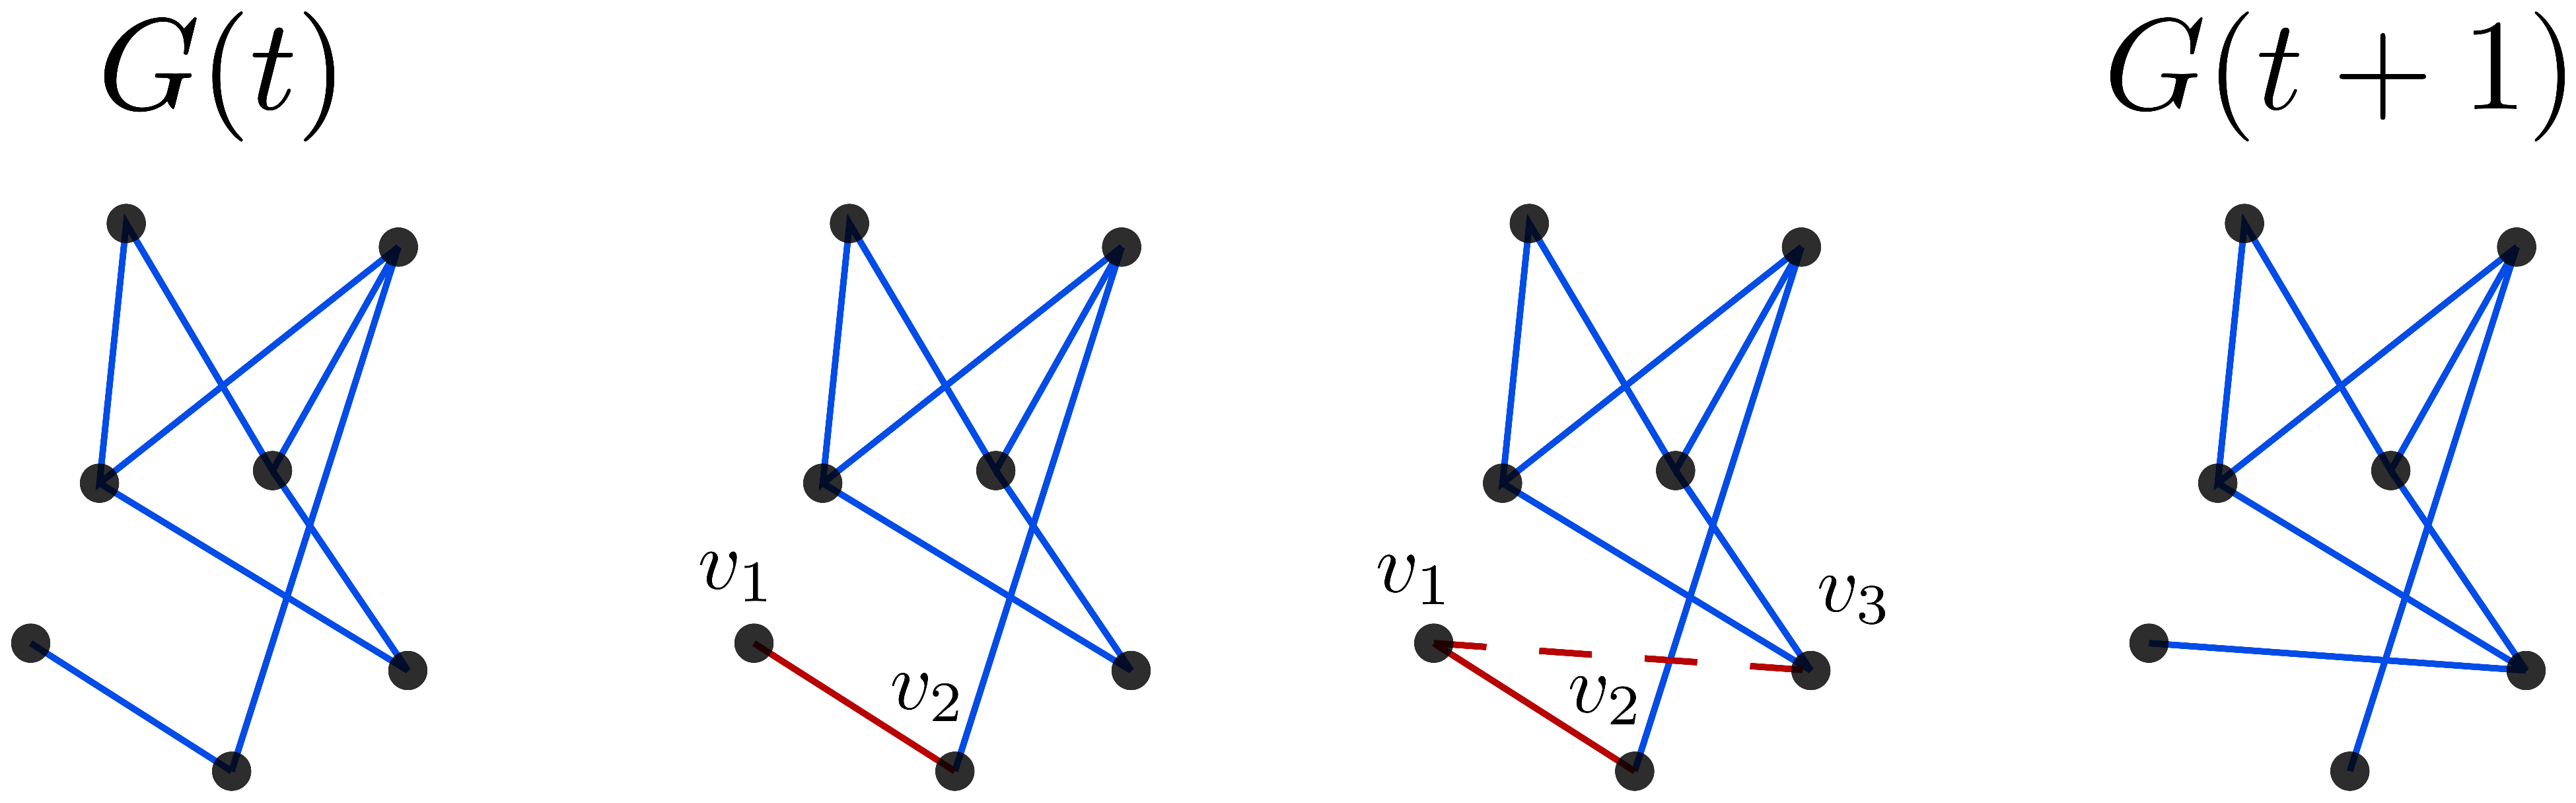
\includegraphics[width=0.9\textwidth]{graph-evo}
    \caption[Schematic of the substeps involved in the multigraph
    evolution dynamics]{Schematic of the substeps of the evolution
      dynamics of the multigraph
      $G(t)$. \label{fig:step-illustration}}
  \end{figure}

  \begin{figure}
    \vspace{-5mm} \centering
    \begin{subfigure}[t]{0.49\textwidth}
      \centering
      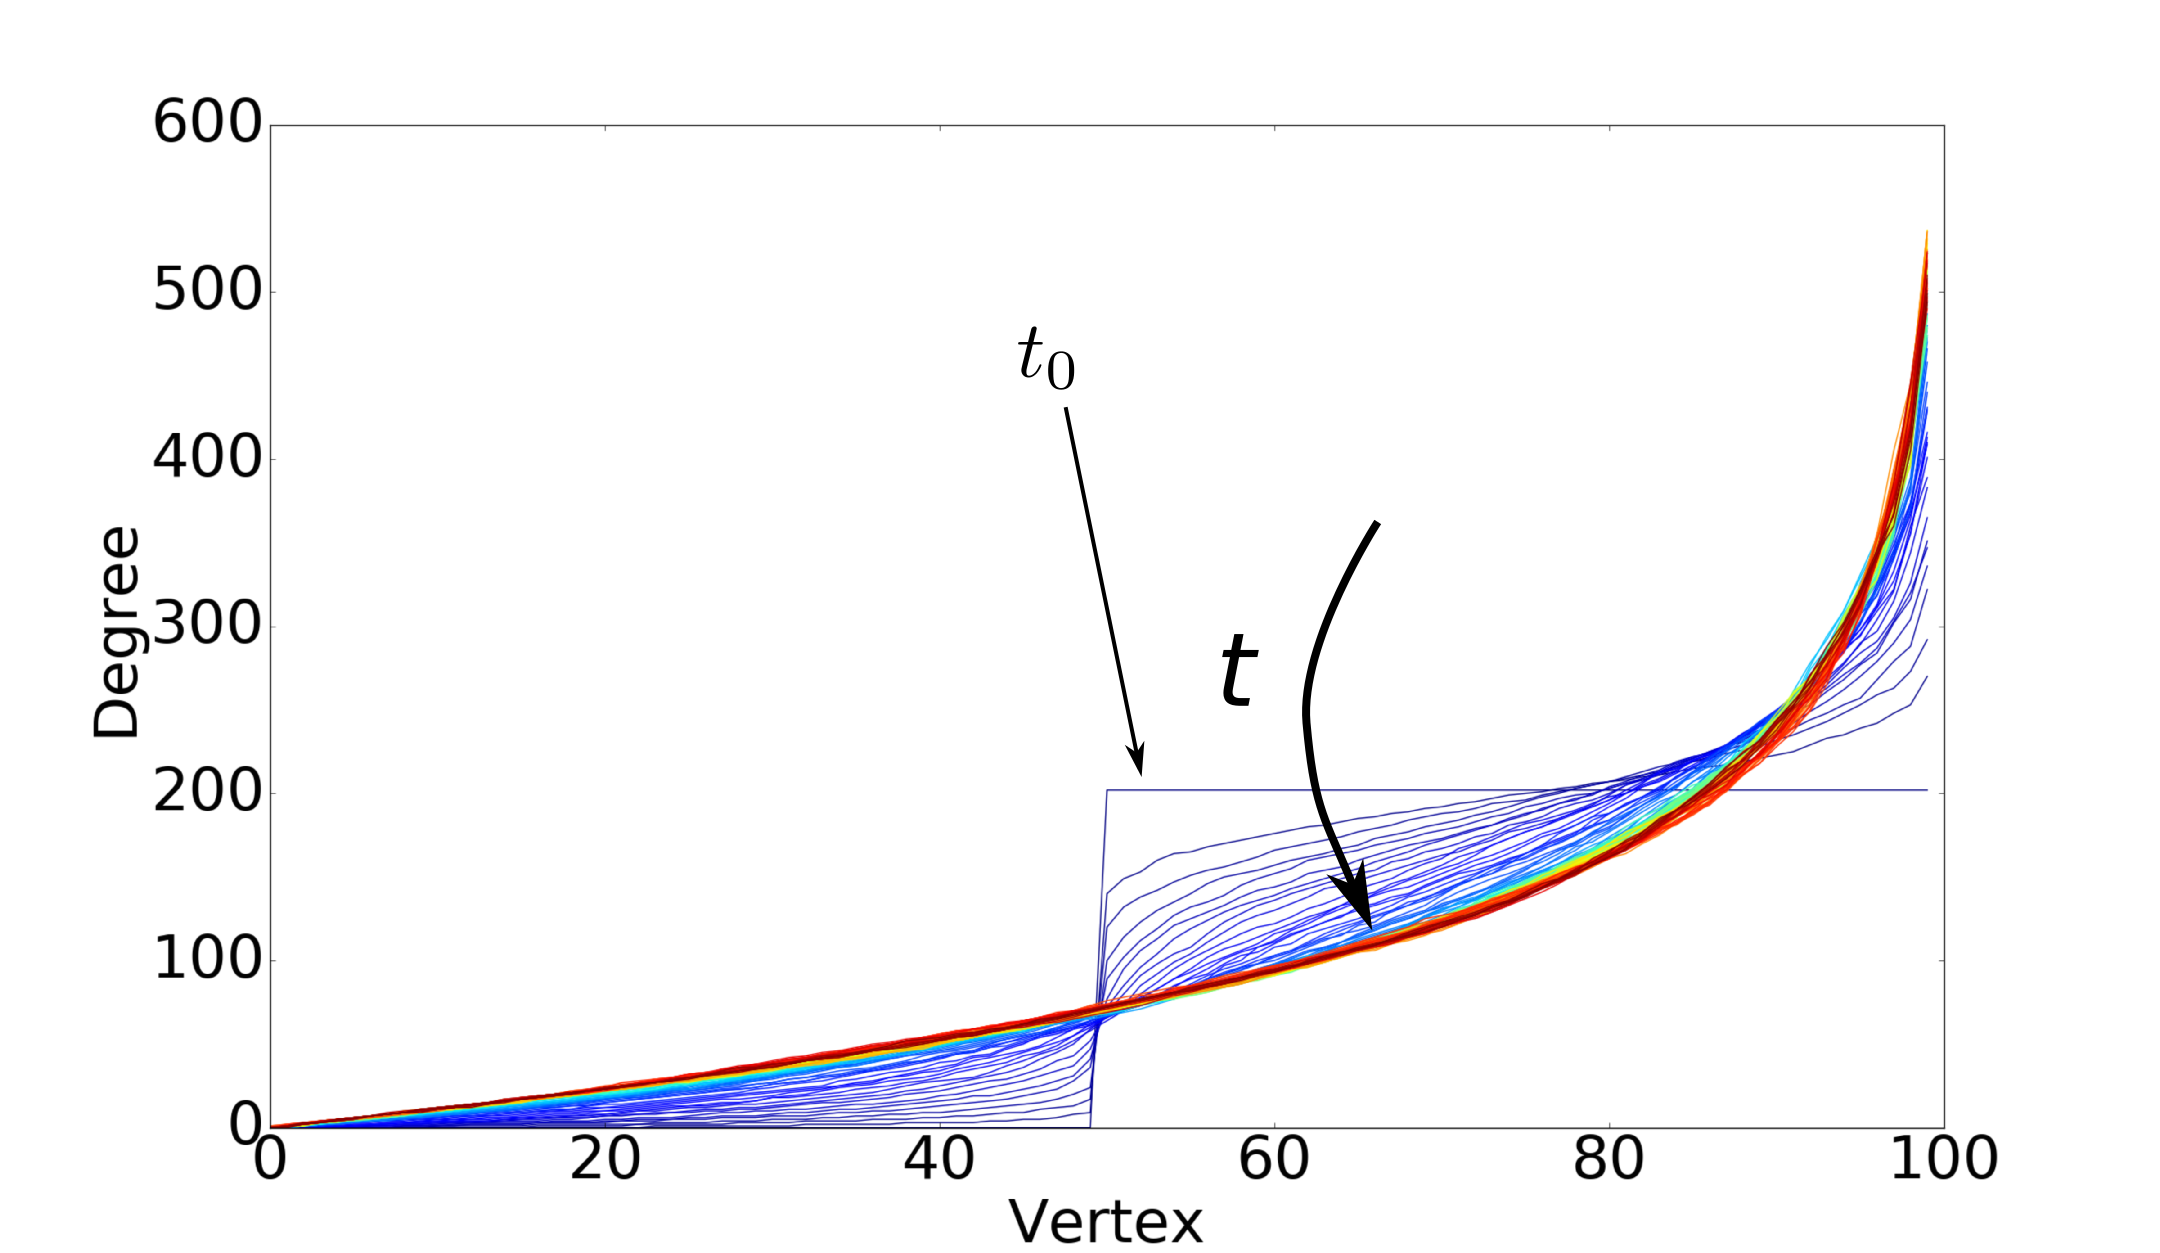
\includegraphics[width=\textwidth]{lopsided-degs-a}
      \subcaption{\label{fig:lopsided-init}}
    \end{subfigure} %
    \begin{subfigure}[t]{0.49\textwidth}
      \centering
      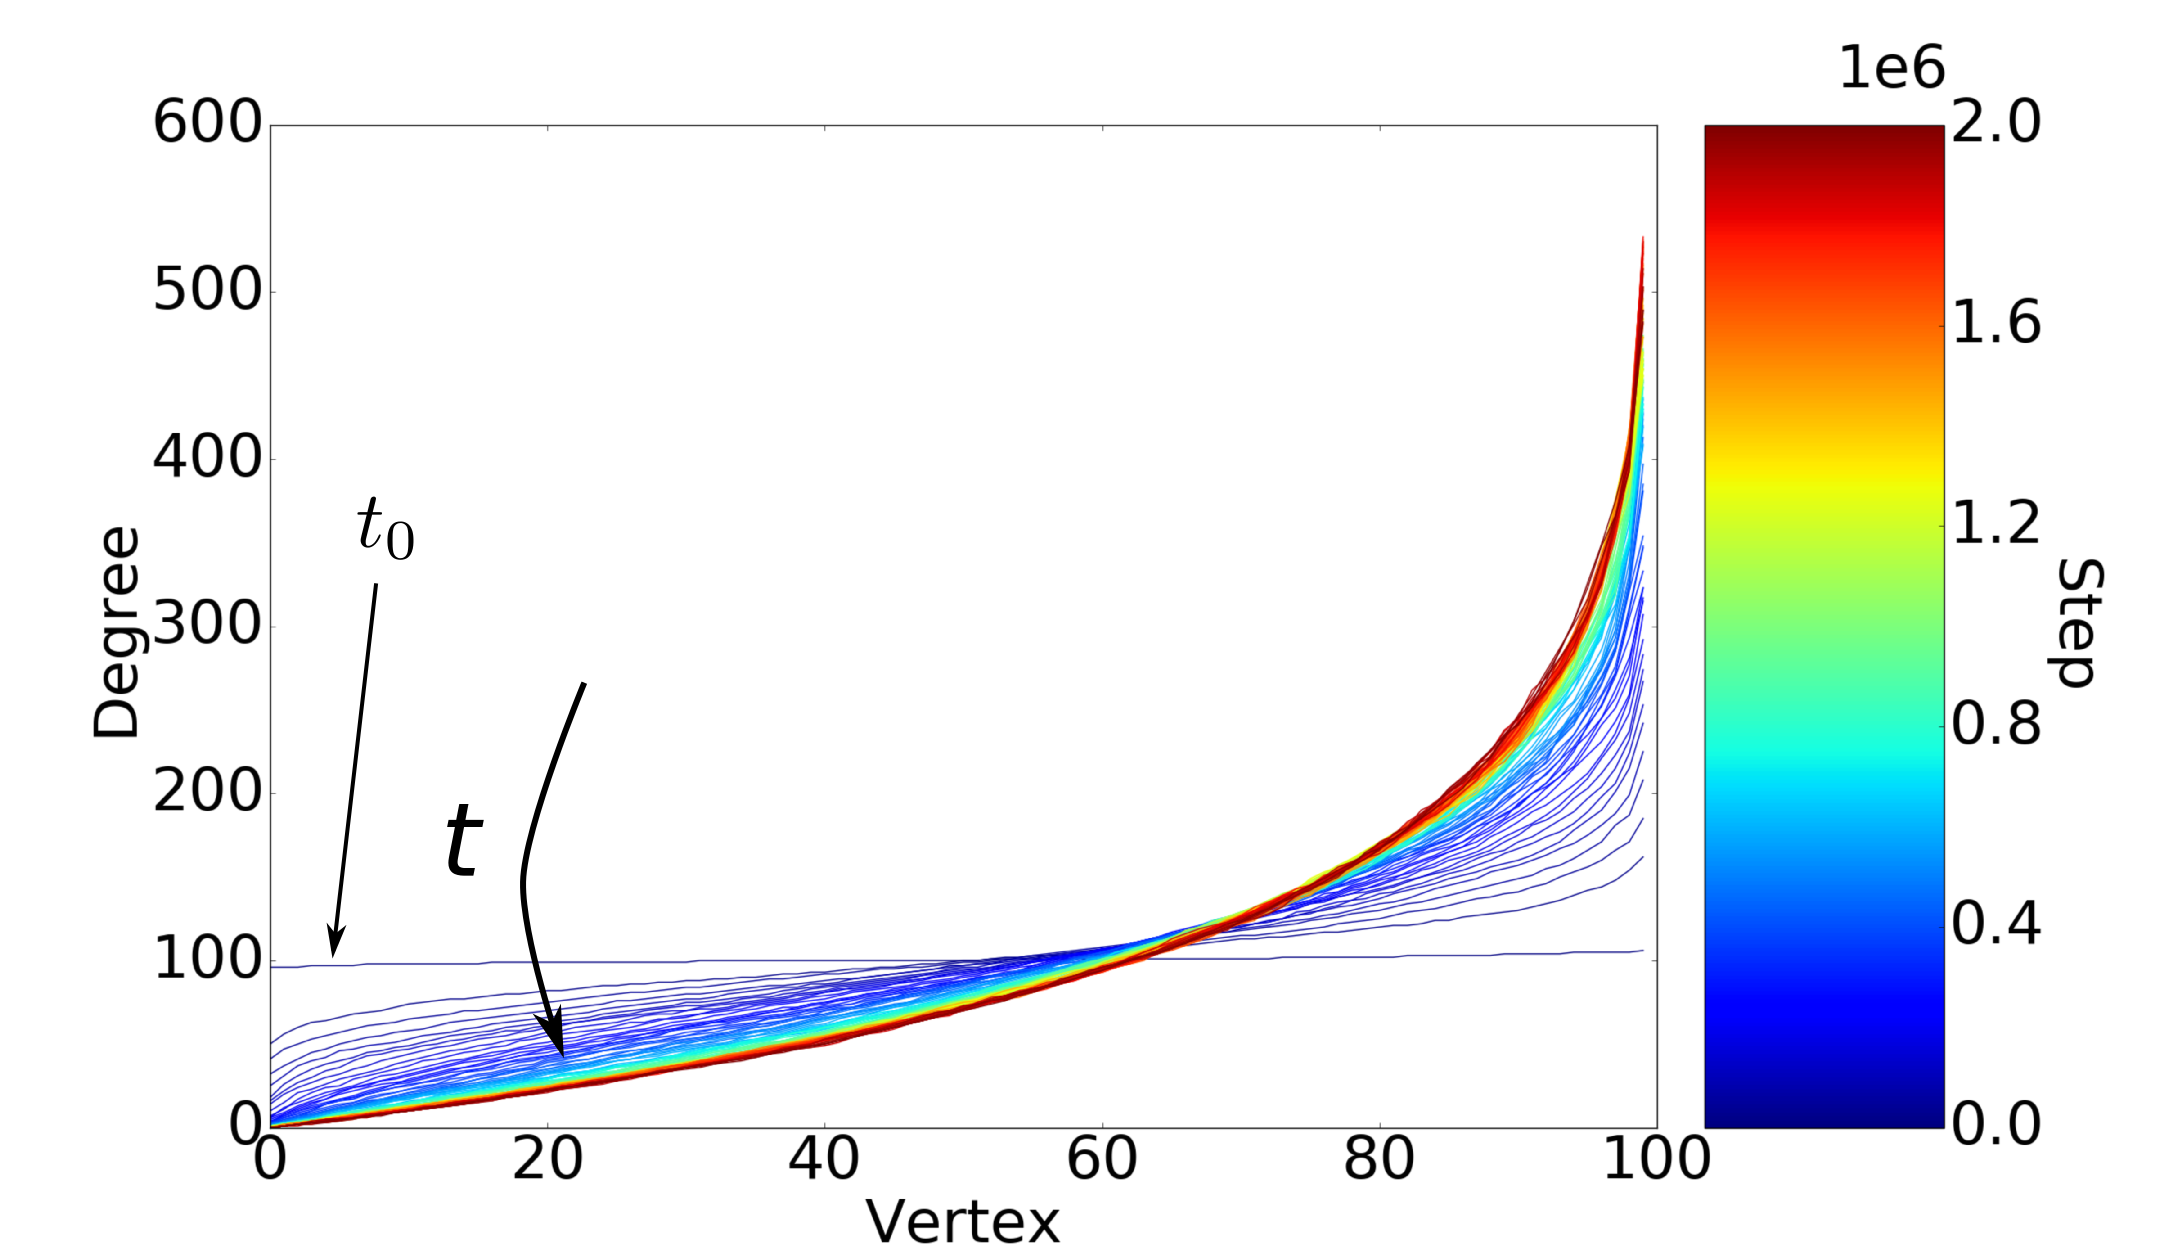
\includegraphics[width=\textwidth]{erdos-degs-a}
      \subcaption{\label{fig:erdos-init}}
    \end{subfigure}
    \caption[Evolution of the multigraph model's sorted degree
    sequence]{Evolution of the multigraph model's sorted degree
      sequence. Two distinct transients are shown, initialized with
      (a) an Erd\H{o}s-R\'{e}nyi random graph with $m = 5,050$ edges
      and (b) a graph in which half the vertices are isolated, and
      half uniformly share $m = 5,050$ edges. Both approach the same
      ultimate stationary sequence. To smoothen the evolution of this
      stochastic system, here we plot the instantaneous average of
      twenty simulations. \label{fig:dse}}
  \end{figure}

  \begin{figure}
    \centering
    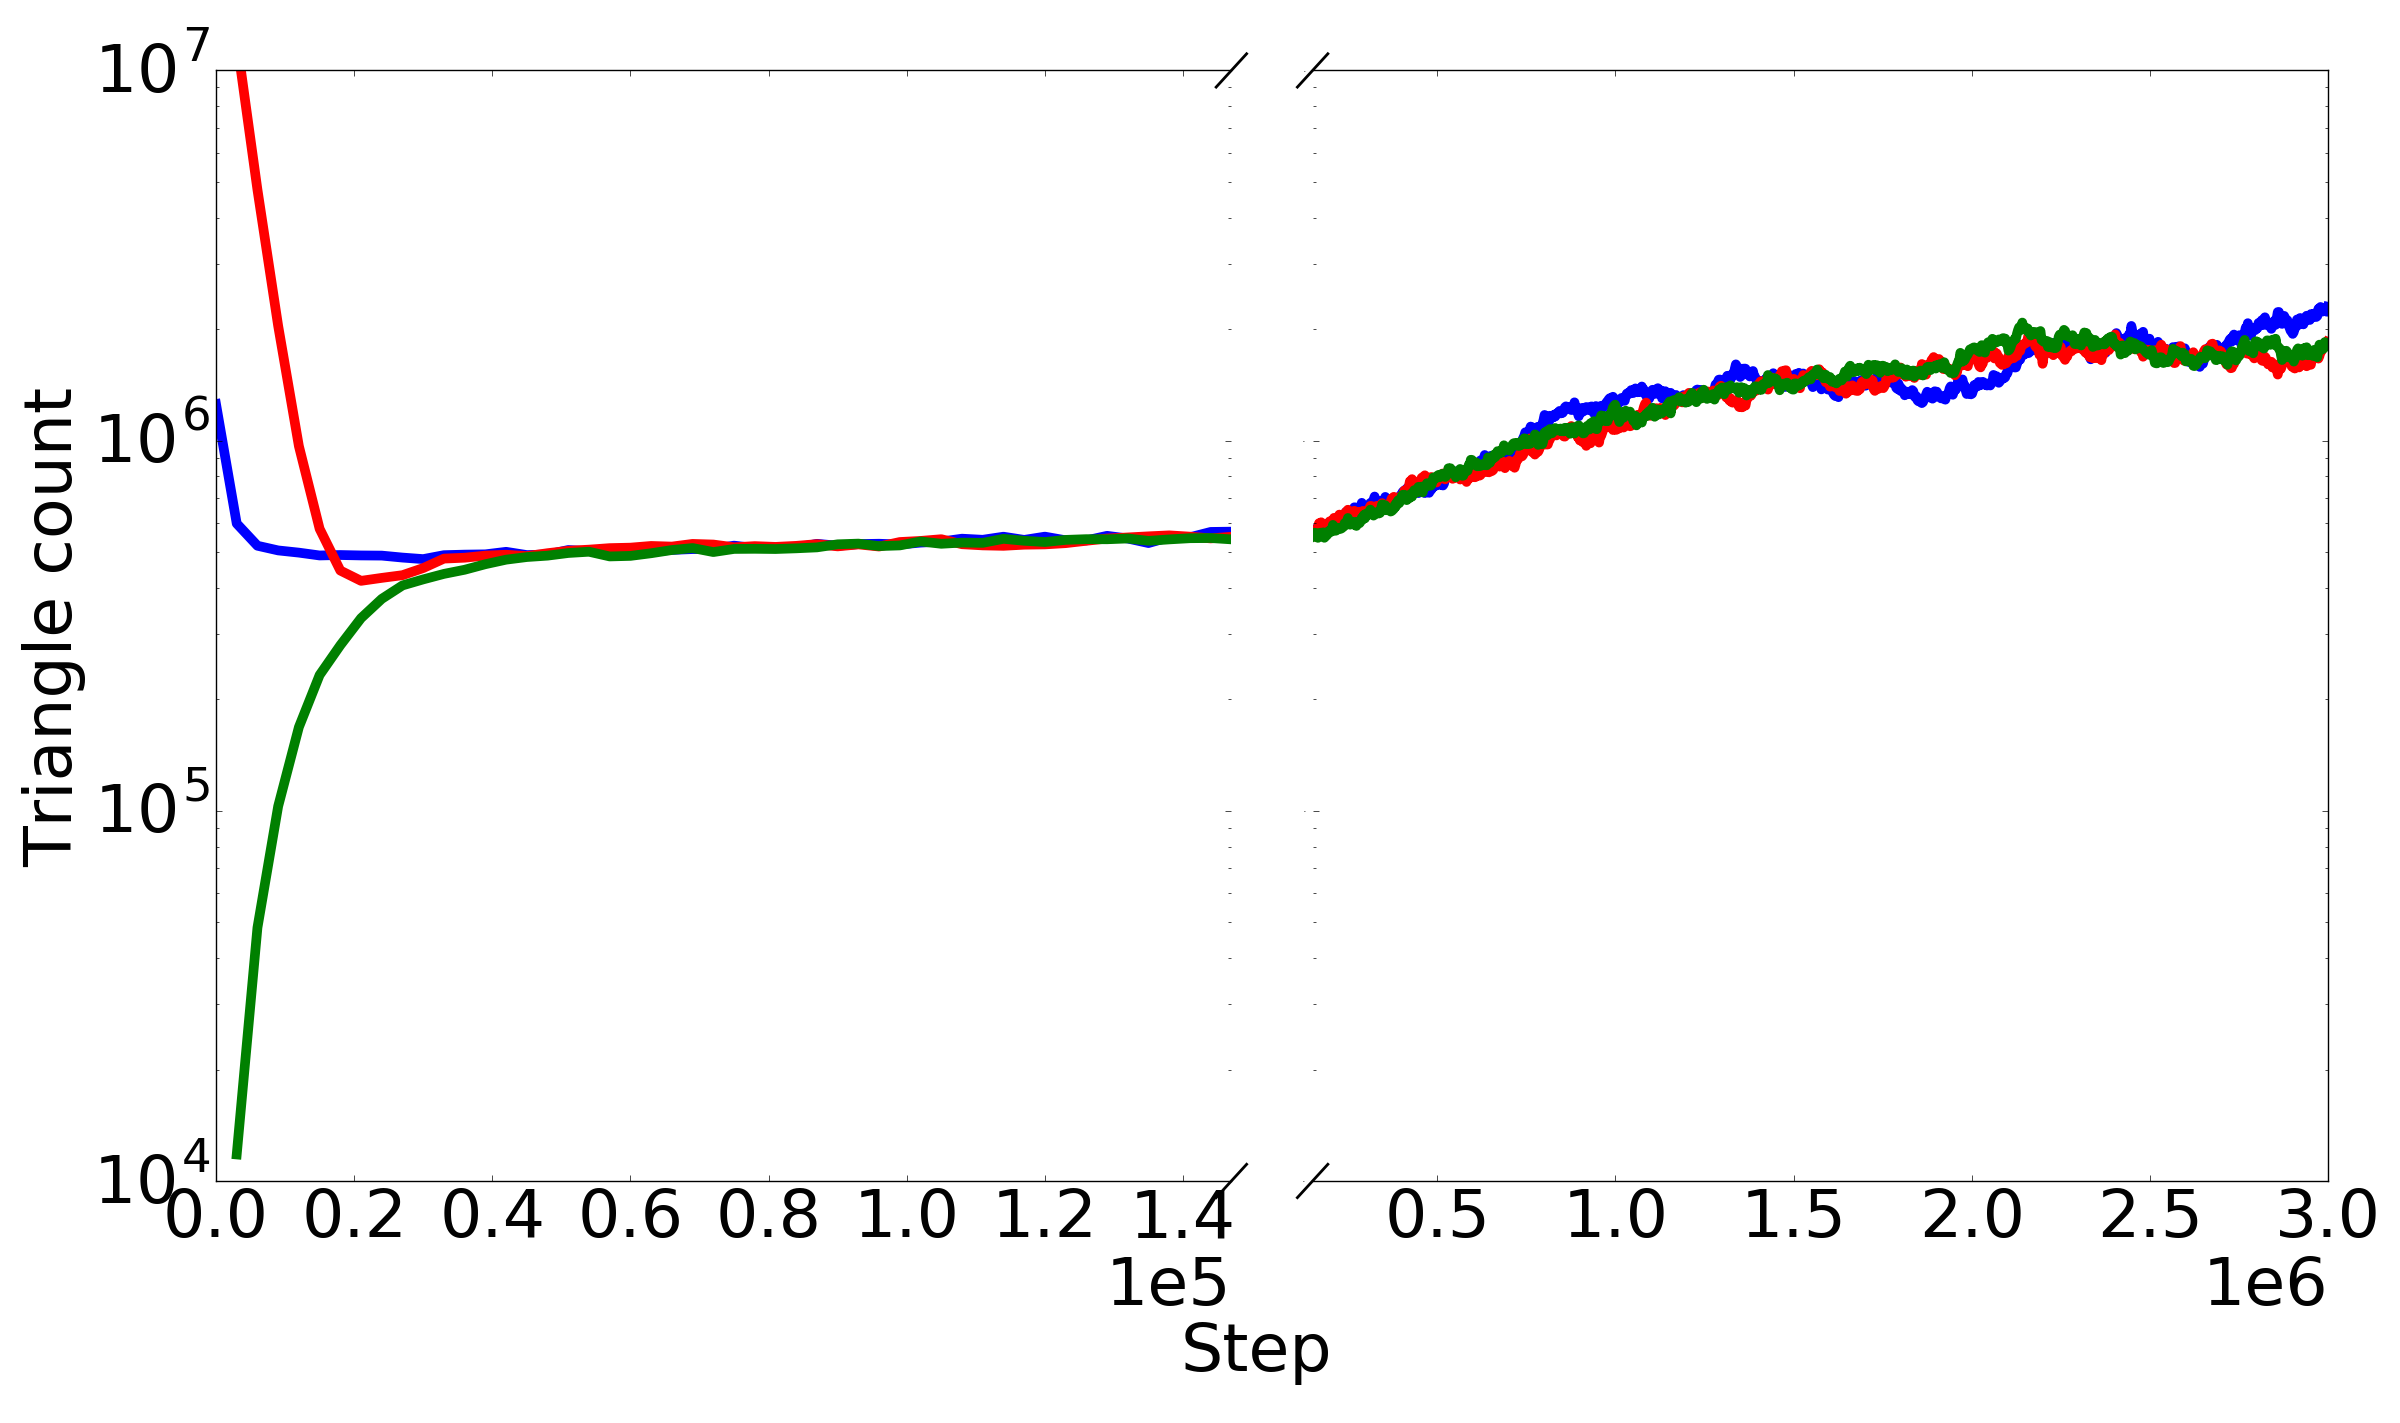
\includegraphics[width=0.8\textwidth]{triangle-slaving-n2-n3}
    \caption[Evolution of triangle count]{Evolution of higher-order
      network statistics (here, the total triangle count) for three
      different network initializations. They are quickly ($O(n^2)$
      steps) drawn to a slow manifold on which they slowly evolve over
      ($O(n^3)$ steps) to a stationary state. \label{fig:sv}}
  \end{figure}

  \section{Equation-free modeling\label{sec:ef}}

  \subsection{Coarse-graining}

  A prerequisite to the implementation of equation-free algorithms is
  the determination of those few, select variables with which one can
  ``close'' a useful approximate description of the coarse-grained
  dynamics of the full, detailed network.
  % 
  This set of variables should clearly be (much) less than those of
  the full system state, and they should evolve smoothly (so, either
  our network would have a large number of nodes, or we would take
  expectations over several realizations of networks with the same
  collective features).
  % 
  Based on the profiles depicted in Fig. (\ref{fig:dse}), the graph's
  degree sequence, (equally informatively, its degree distribution) is
  a good candidate collective observable.
  % 
  It appears to evolve smoothly, while also providing significant
  savings in dimensionality, from an $O(n^2)$ adjacency matrix to a
  length-$n$ vector of degrees. \par

  It now becomes crucial to test whether the evolution of other
  properties of the graph can be correlated to the degree sequence.
  % 
  If not, our current description is incomplete (an equation cannot
  close with only the degree sequence) and there exist other important
  coarse variables that must be included in our macroscopic system
  description.
  % 
  To assess this, we constructed graphs with identical degree
  sequences but varying triangle counts and recorded the evolution of
  this observable under the dynamics prescribed in Section
  \ref{sec:m}. Fig. (\ref{fig:sv}) shows that, within a short time,
  the triangle counts are drawn to an apparent shared ``slow
  manifold'', despite the variation in initial conditions.
  % 
  This supports our selection of the degree sequence as an adequate
  coarse variable to model the system. \par

  Next we describe the other two key elements to equation-free
  modeling which map to and from our microscopic and macroscopic
  descriptions: restriction and lifting operators.

  \begin{figure}
    \centering
    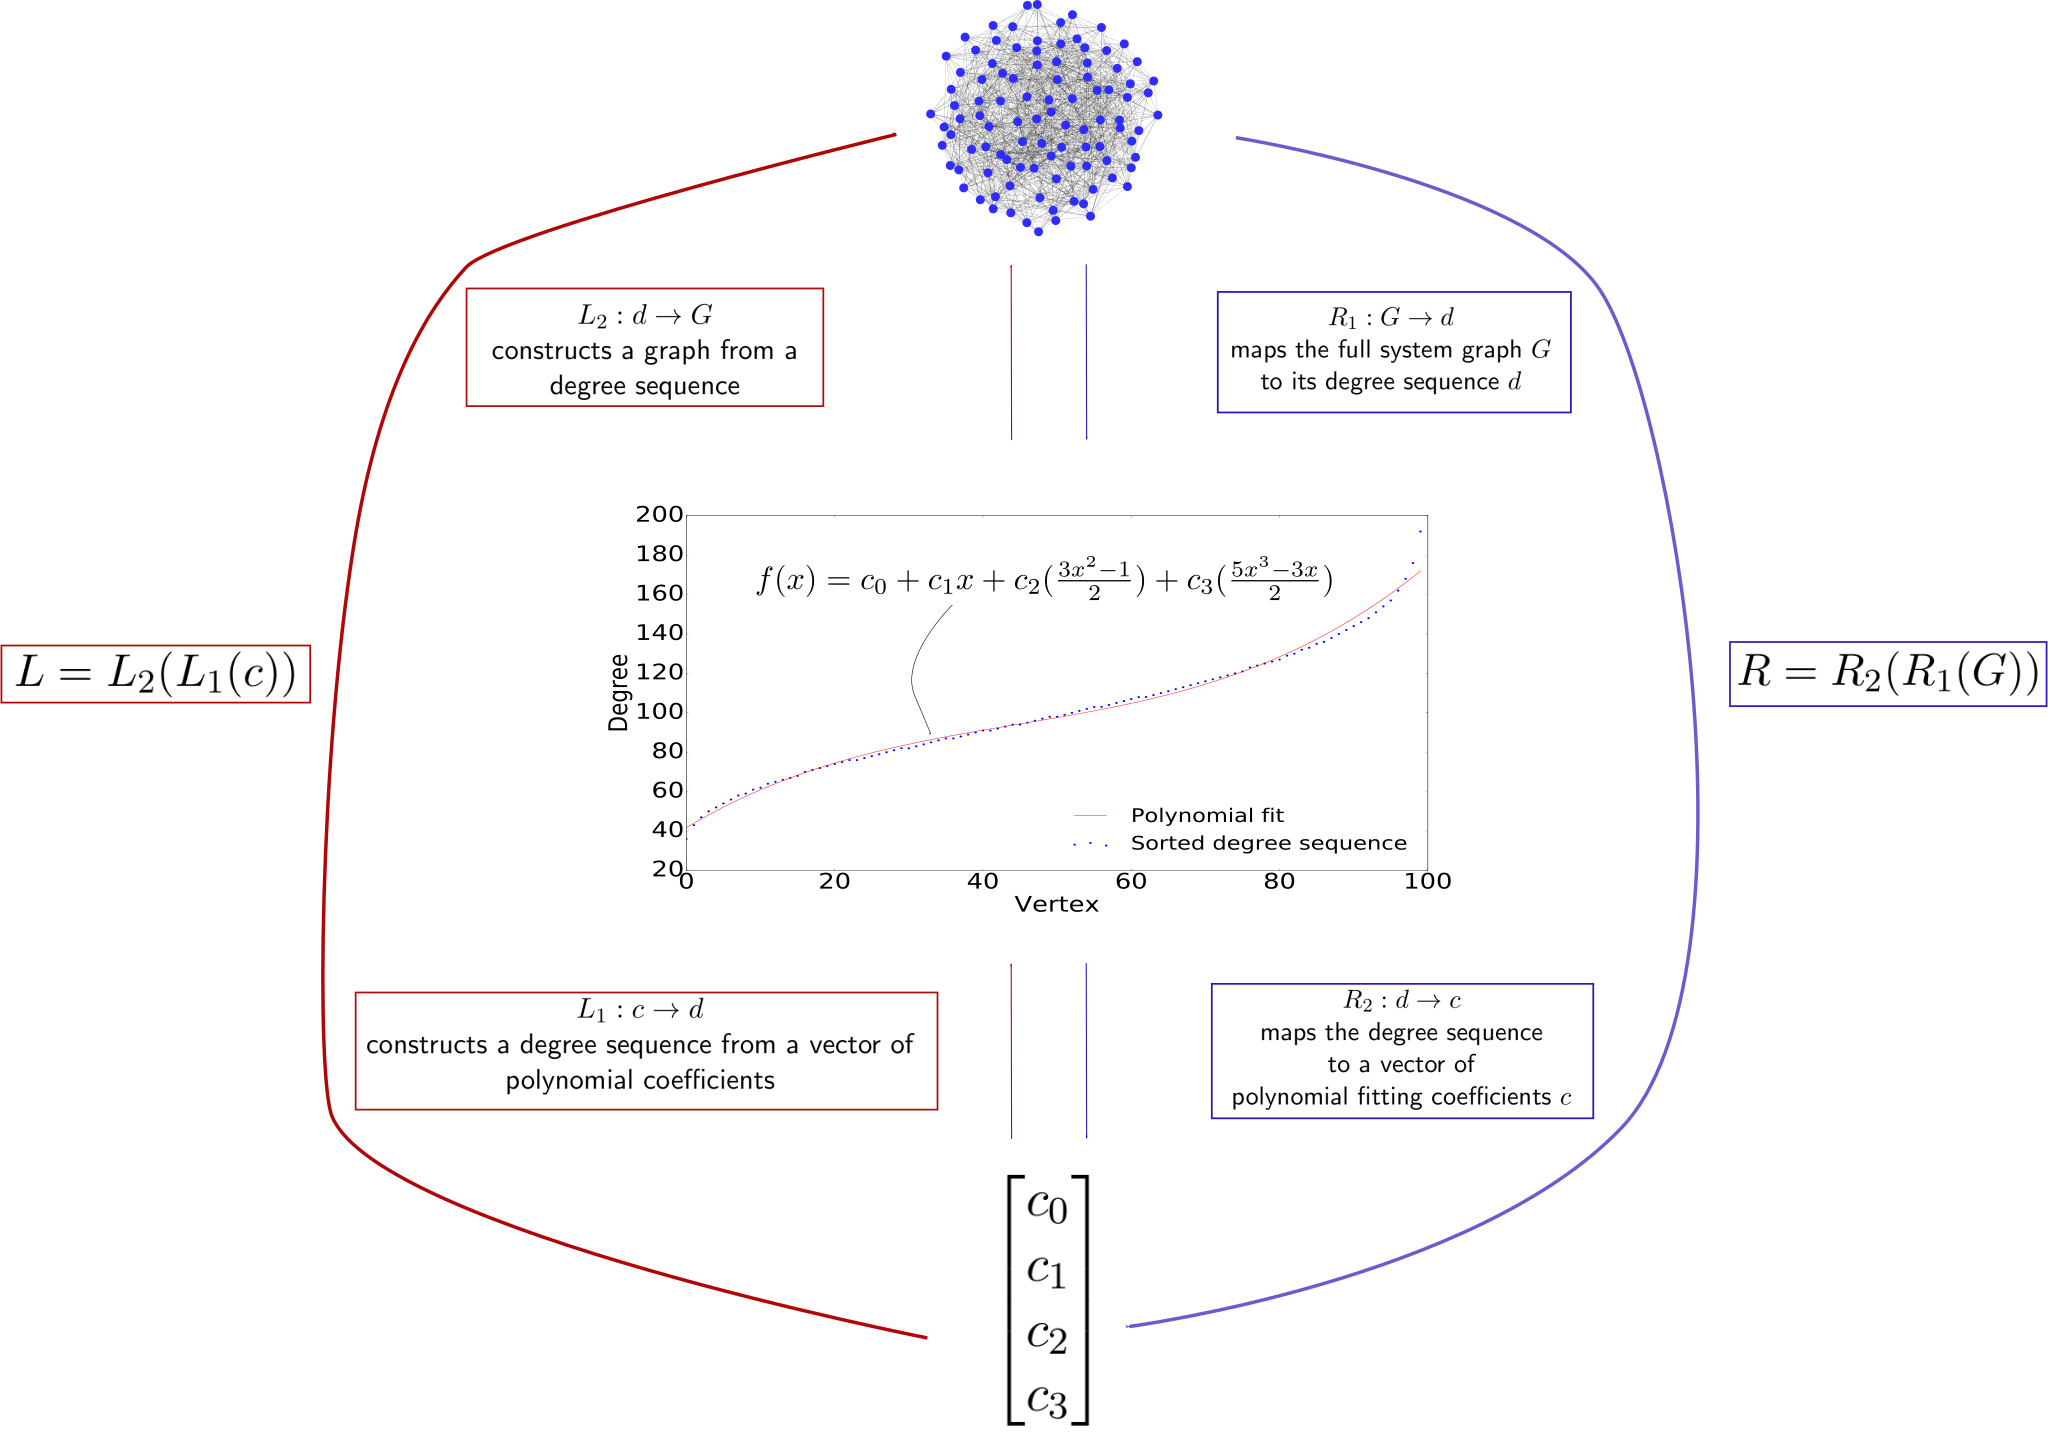
\includegraphics[width=\textwidth]{cpi-diagram}
    \caption[Schematic of multigraph's lifting and restricting
    procedures]{Schematic of our restriction ($\mathbf{R}$) and
      lifting ($\mathbf{L}$) procedures. The graph's sorted degree
      sequence is calculated ($R_1$) and then fit to a third-order
      polynomial ($R_2$). This maps graphs ($G$) to vectors of four
      coefficients ($\mathbf{c}$). To lift, the polynomial is used to
      generate a degree sequence ($L_1$), which is then used to
      construct a consistent graph ($L_2$). This process maps vectors
      of four coefficients ($\mathbf{c}$) to graphs ($G$).
      $\mathbf{R} = R_2 \circ R_1 $ is our restriction and
      $\mathbf{L} = L_2 \circ L_1$ is our
      lifting. \label{fig:cpi-diagram}}
  \end{figure}


  \subsection{Restriction}

  The restriction operator ``translates'' the full network description
  to its corresponding coarse variable values.
  % 
  Here, this involves mapping a multigraph to its sorted degree
  sequence, a simple calculation.
  % 
  However, we may be able to further reduce the dimensionality of our
  coarse system by keeping not the entire length-$n$ degree sequence,
  but rather a low-order polynomial fitting of it.
  % 
  To do so, we first sort the sequence to achieve a smooth,
  monotonically increasing dataset, then fit the result to a
  third-order polynomial, which had been observed to closely
  approximate the sequence evolution throughout time.
  % 
  Our coarse description thus consisted, at every moment in time, of
  the four polynomial coefficient values, specifying a particular
  sorted degree sequence, as shown in Fig. (\ref{fig:cpi-diagram}).
  % 
  The restriction operator therefore maps multigraphs to length-four
  coefficient vectors.
  % 
  This procedure is represented by the blue arrows of
  Fig. (\ref{fig:cpi-diagram}).

  \subsection{Lifting}

  The lifting operator performs the inverse role of restriction:
  translating coarse variables into full networks.
  % 
  This is clearly a one-to-many mapping.
  % 
  Specifically in the context of our model, we map vectors of
  polynomial coefficients to full networks in a two-stage process.
  % 
  First, the coefficient vector is used to recreate a sorted degree
  sequence by evaluating the full polynomial at integer values and
  rounding to the nearest degree, as depicted in
  Fig. (\ref{fig:cpi-diagram}).
  % 
  If the sum of the resulting degree sequence is odd, a single degree
  is added to the largest value to ensure the sequence is graphical.
  % 
  Second, this degree sequence is used as input to any algorithm that
  produces a network consistent with a graphical degree sequence (here
  we typically used a Havel-Hakimi algorithm, creating a graph whose
  degree sequence matches that of the input
  \cite{havel_remark_1955,hakimi_realizability_1962}).
  % 
  While the canonical Havel-Hakimi method produces simple graphs, it
  is not difficult to extend it to multigraphs by allowing the
  algorithm to wrap around the sequence, producing multiple edges and
  self-loops.  The lifting procedure is represented by the red arrows
  of Fig. (\ref{fig:cpi-diagram}).

  \subsection{Coarse projective integration (CPI)}
  \label{sec:cpi}

  The components described above are combined to accelerate
  simulations through Coarse Projective Integration.
  % 
  Denoting the lifting operator by
  $\mathbf{L} \; : \; c \rightarrow G$ where $c \in \mathbb{R}^4$ is
  the vector of polynomial coefficients, and the restriction operator
  as $\mathbf{R} \; : G \rightarrow c$, the algorithm progresses as
  follows:

  \begin{enumerate}
  \item Advance the full system for $t_h$ steps
    \label{cpi:heal}
  \item Continue for $t_c$ steps, restricting the network at intervals
    and recording the coarse variable values
  \item Using the coarse variables collected over the previous $t_c$
    steps, project each variable forward $t_p$ steps with, here, a
    forward-Euler method
    \label{cpi:proj}
  \item With the new, projected coarse variables, lift to one (or more
    copies of) full network
    \label{cpi:init}
  \item Repeat from Step (\ref{cpi:heal}) until the desired time has
    been reached.
  \end{enumerate}

  Note that Step (\ref{cpi:heal}) is intended to allow a singularly
  perturbed quantity to approach its slow manifold.
  % 
  Upon initializing a new full system (here, a new network) in Step
  (\ref{cpi:init}), higher order observables (for example, the
  triangle count) will be far from the values they would attain in a
  detailed simulation.
  % 
  If the coarse system model closes with our chosen variables, then
  either (a) these quantities do not affect the dynamics of the degree
  sequence; or (b) they do, but then by hypothesis these quantities
  quickly evolve to functions of the selected coarse variables (i.e.,
  they approach the slow manifold).
  % 
  In the second case, after a short interval of ``healing'' they will
  be drawn to the expected trajectory, after which we begin sampling.
  % 
  This is analogous to Fig. (\ref{fig:sv}).
  % 
  The computational gains arise from the projective step,
  (\ref{cpi:proj}).
  % 
  Here, we advance the system $t_p$ steps at the cost of one
  evaluation of forward Euler, instead of $t_p$ direct detailed steps.

  Results of the application of this general framework with the
  specific lifting and restriction operators previously outlined are
  shown in Fig. (\ref{fig:cpi-results}). We used an $n=100$-vertex
  graph with $m=50000$ edges and parameter value $\kappa=1$. We ran
  the model for a total of $10 \cdot n^3$ steps, with
  $t_h = 10 \cdot n^2$, $t_c = n^3$ and $t_p = 50 \cdot n^2$.
  % 
  We see good agreement between the CPI-accelerated and normal
  systems, while reducing the number of detailed steps by one third.
  % 
  It is important to mention that this method was applied not to a
  single system instantiation, but to an ensemble of fifty such
  realizations.  This ensured that when properties such as the fitted
  polynomial coefficients were averaged over the ensemble they evolved
  smoothly despite the stochastic nature of the system; in effect, we
  are computing the ``expected network evolution'' averaged over
  consistent realizations.

  \begin{figure}
    \vspace{-5mm} \centering
    \begin{subfigure}{0.59\textwidth}
      \centering
      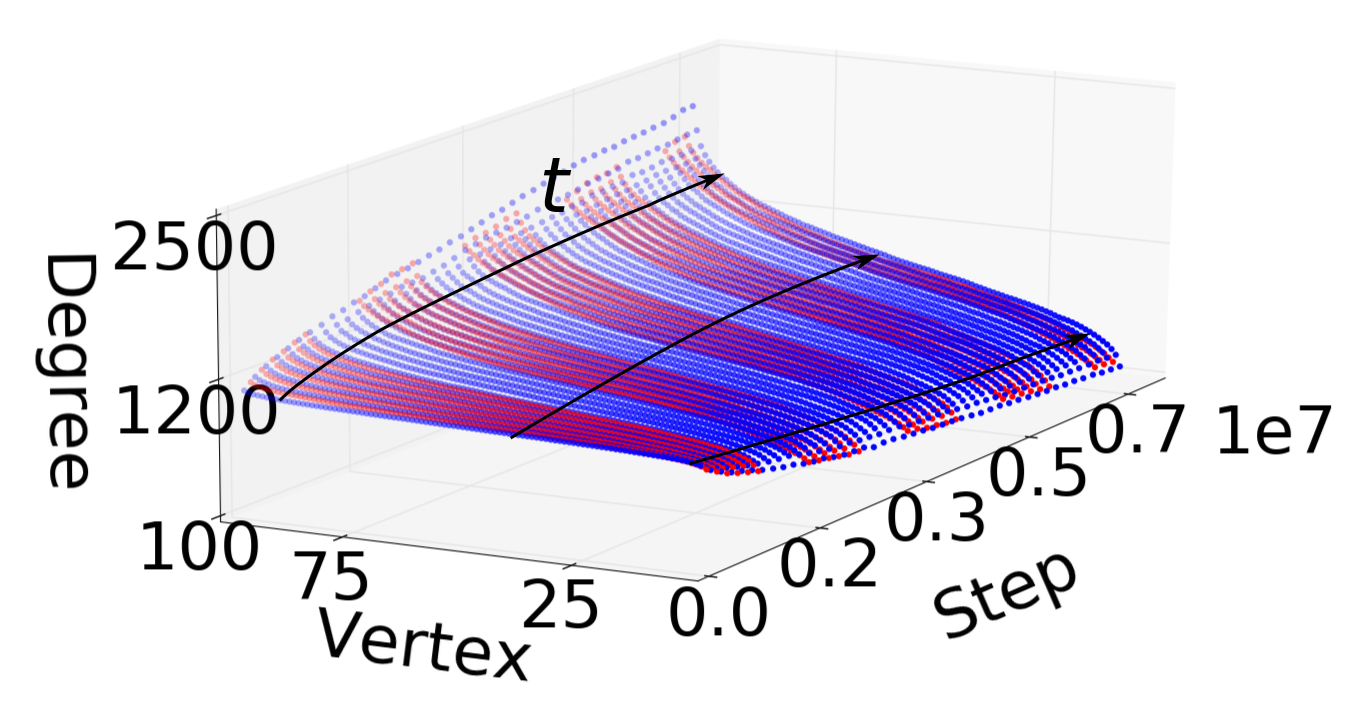
\includegraphics[width=\textwidth]{cpi-3d-comp-stretch}
      \subcaption{\label{fig:cpi-error}}
    \end{subfigure} %
    \begin{subfigure}{0.39\textwidth}
      \centering
      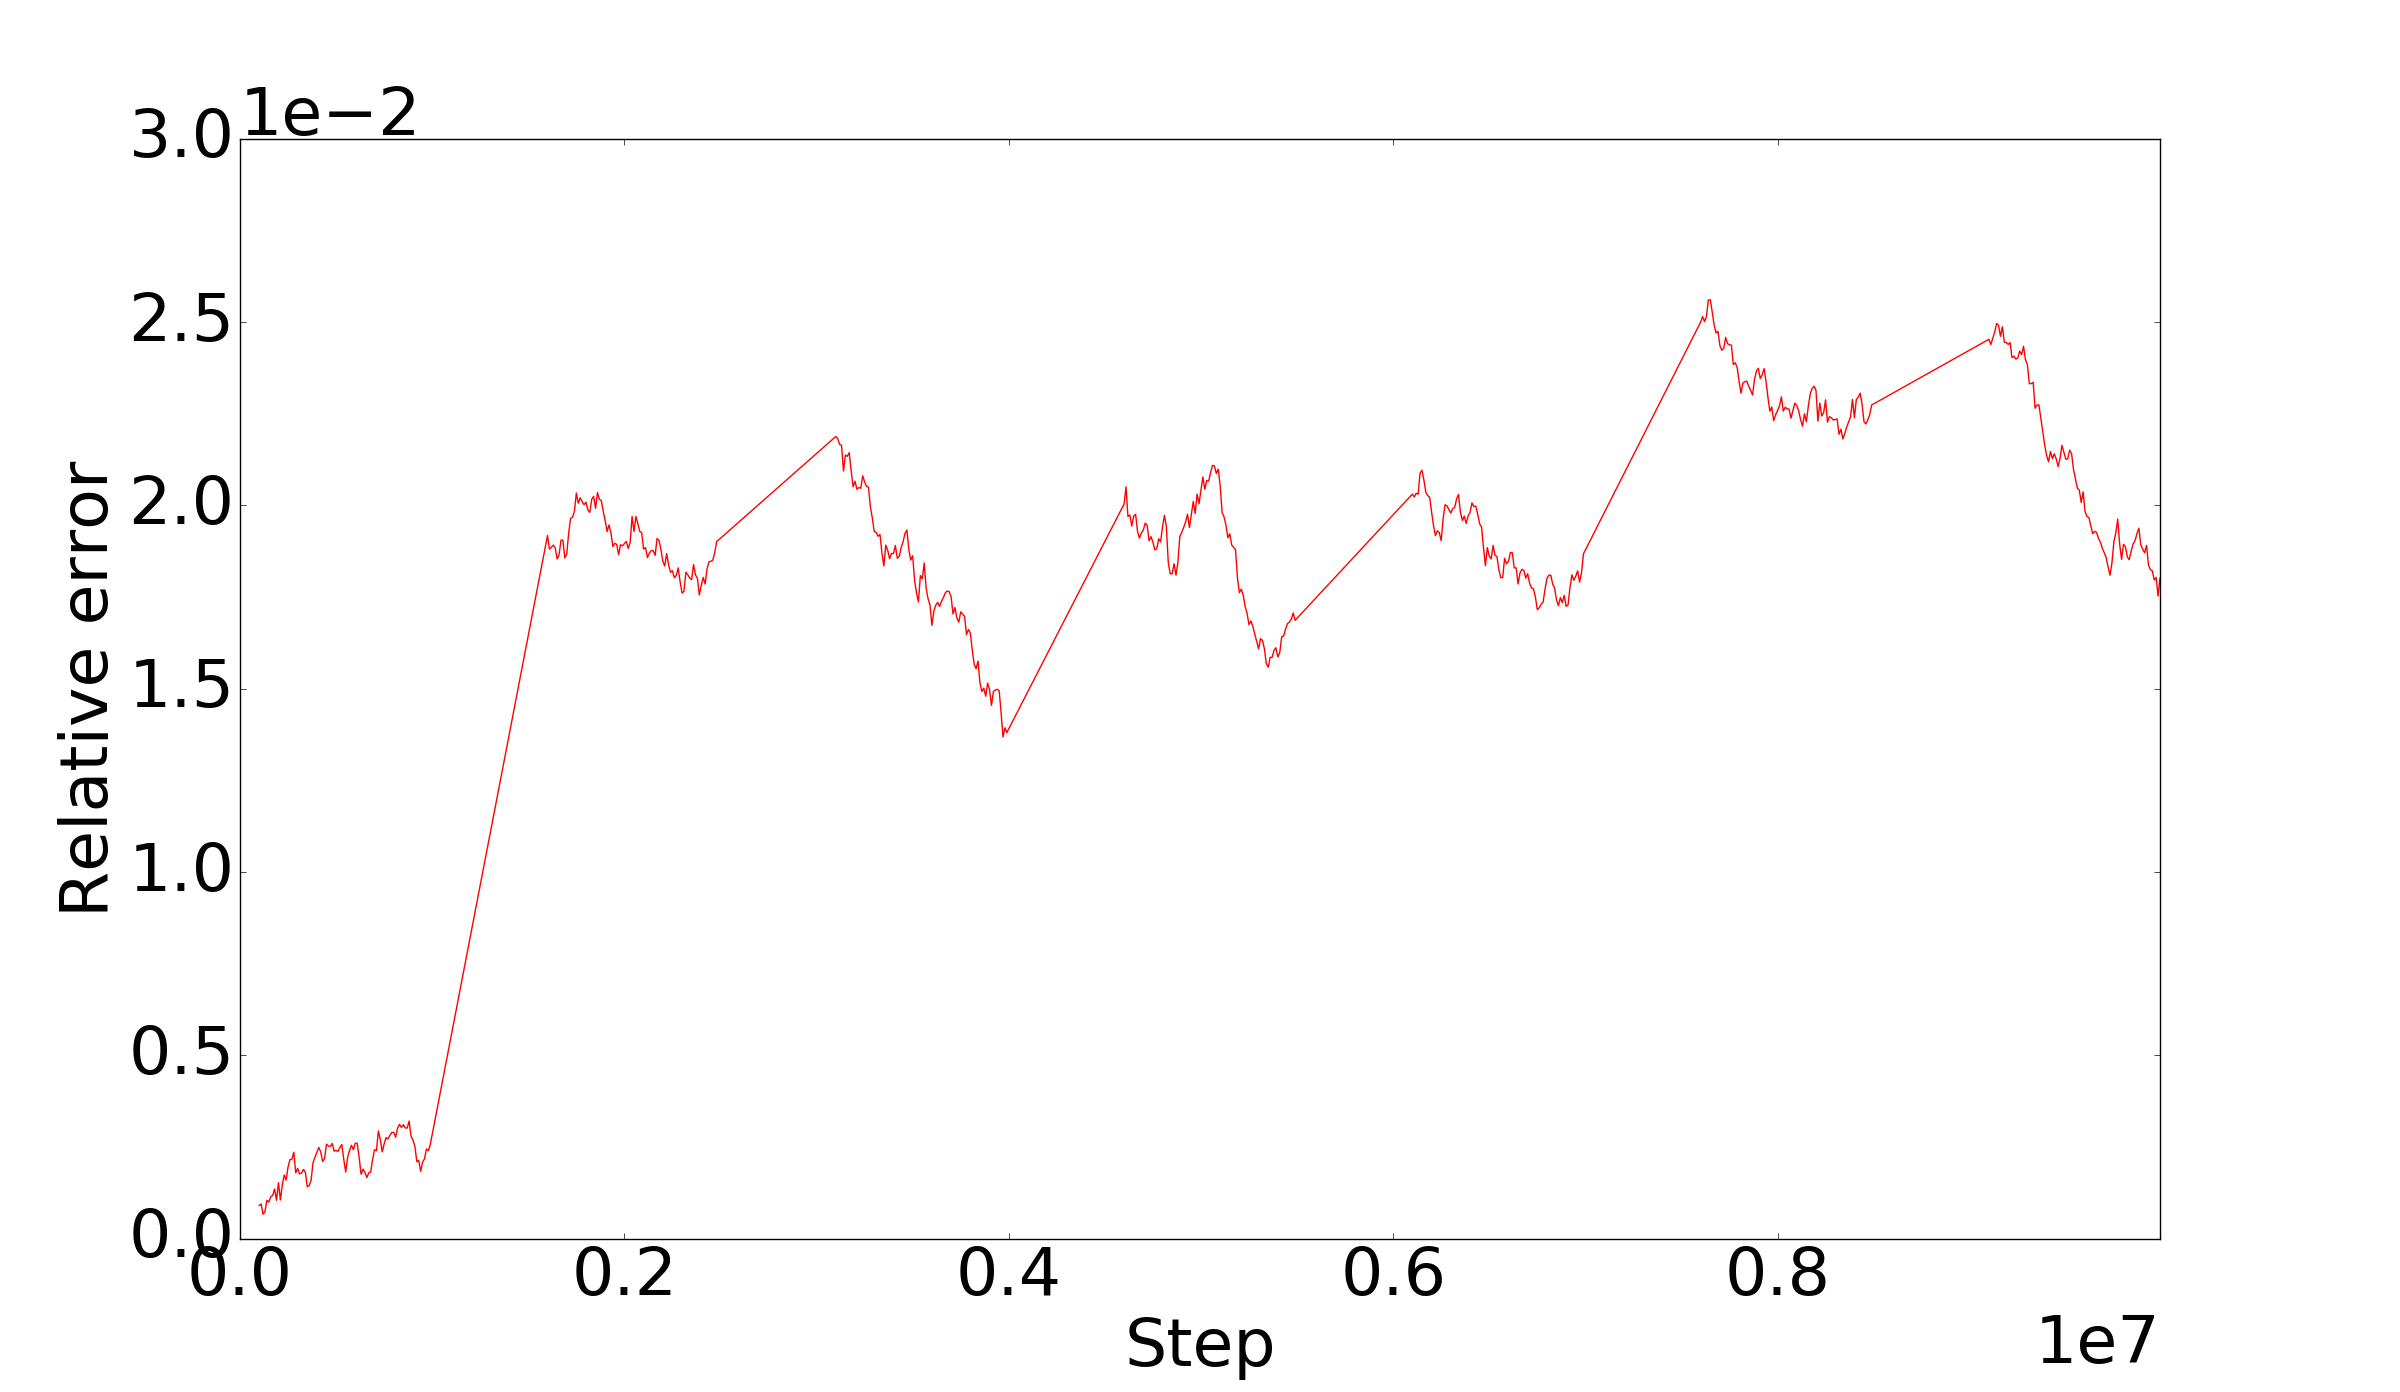
\includegraphics[width=\textwidth]{cpi-relative-error-n3}
      \subcaption{\label{fig:self-error}}
    \end{subfigure}%
    \caption[Coarse-projective integration results]{CPI results: (a)
      the evolution of the CPI-accelerated degree sequence (red)
      compared to direct simulation (blue) and (b) error in
      CPI-accelerated runs calculated by comparing CPI-accelerated
      degree sequences to those arising from an ensemble of direct
      simulations. \label{fig:cpi-results}}
  \end{figure}


  \section{Coarse Newton-GMRES}
  \label{sec:ng}
  Aside from the computational savings of model simulations offered by
  CPI, the equation free framework also permits the calculation of
  system steady states through fixed point (here, matrix-free
  Newton-GMRES) algorithms.
  % 
  Referring back to the CPI procedure outlined in
  Sec. (\ref{sec:cpi}), we can define an operator
  $\Theta: \mathbf{d} \rightarrow \mathbf{d}$ projecting coarse
  variables at $t$ to their values at $t + \delta t$:
  $\mathbf{d}(t+\delta t) =\Theta(\mathbf{d}(t))$.
  % 
  Note that in this section, we take the sorted degree sequence as our
  coarse variable.
  % 
  A system fixed point could then be located by employing Newton's
  method to solve the equation

  \begin{align}
    \label{eq:f}
    \mathbf{F}(\mathbf{d}) \equiv \Theta(\mathbf{d}) - \mathbf{d} = 0
  \end{align}

  However, this requires the repeated solution of the system of linear
  equations
  $DF(\mathbf{d}^{(k)}) \cdot \delta \mathbf{d}^{(k+1)} =
  -\mathbf{F}(\mathbf{d}^{(j)})$, in which the system Jacobian, $DF$
  is unavailable.
  % 
  Thankfully, we may circumvent this obstacle by estimating the
  directional derivatives $DF(\mathbf{d}) \cdot \delta \mathbf{d}$ via
  a difference approximation of the form

  \begin{align}
    DF(d) \cdot \delta \mathbf{d} \approx \frac{\| \delta \mathbf{d} \| \mathbf{F}(\mathbf{d} + h \| \mathbf{d} \| \frac{\delta \mathbf{d}}{\| \delta \mathbf{d} \|}) - \mathbf{F}(\mathbf{d})}{h \| \mathbf{d} \|}
  \end{align}

  \noindent for nonzero $\mathbf{d}$, which in turn is evaluated
  through calls to $\mathbf{F}$ as defined in Eq. (\ref{eq:f})

  This is precisely the approach of the Newton-GMRES method, in which
  the solution to a linear system is sought for in expanding Krylov
  subspaces \cite{kelley_solving_2003}.
  % 
  Applying this algorithm in conjunction with the $\Theta$ operator
  defined in Sec. (\ref{sec:cpi}) allowed us to locate the stationary
  distribution without simply running and observing the full system
  for long times, as would otherwise be required.
  % 
  Results are shown in Fig. (\ref{fig:newton-results}).
  % 
  We note that coarse stability results can also be obtained via an
  iterative Arnoldi eigensolver, again estimating matrix-vector
  products as above.

  \begin{figure}
    \vspace{-5mm} \centering
    \begin{subfigure}{0.49\textwidth}
      \centering
      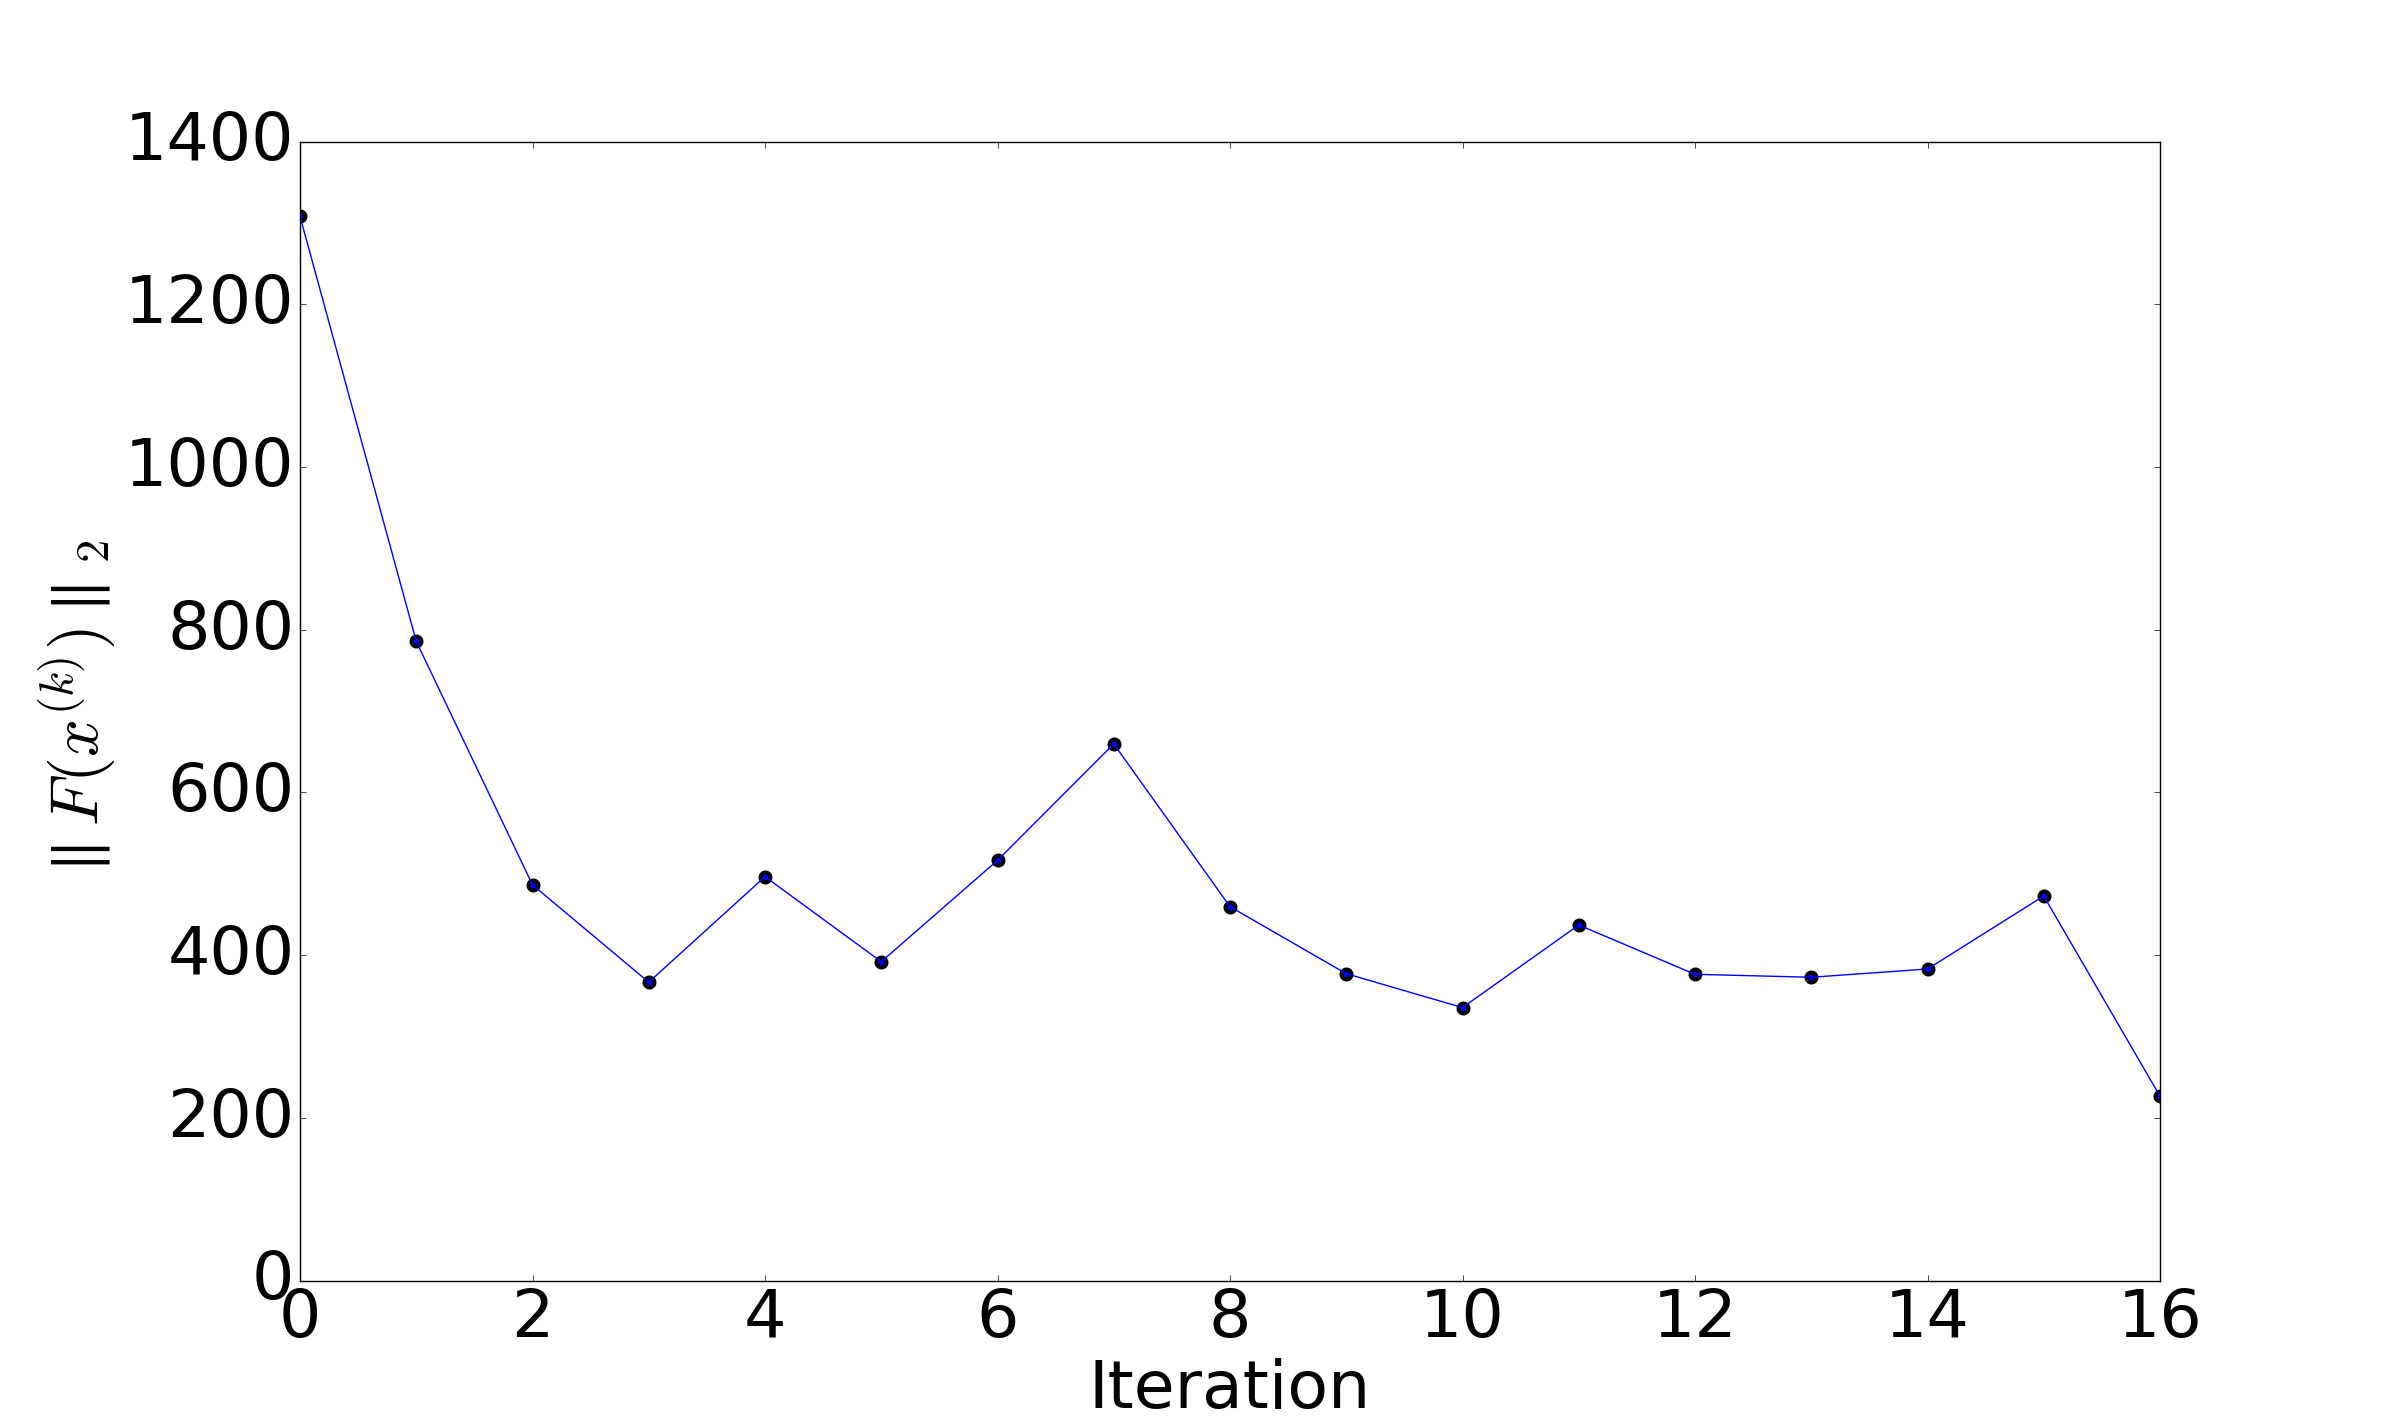
\includegraphics[width=\textwidth]{newton-error}
      \subcaption{\label{fig:newton-error}}
    \end{subfigure} %
    \begin{subfigure}{0.49\textwidth}
      \centering
      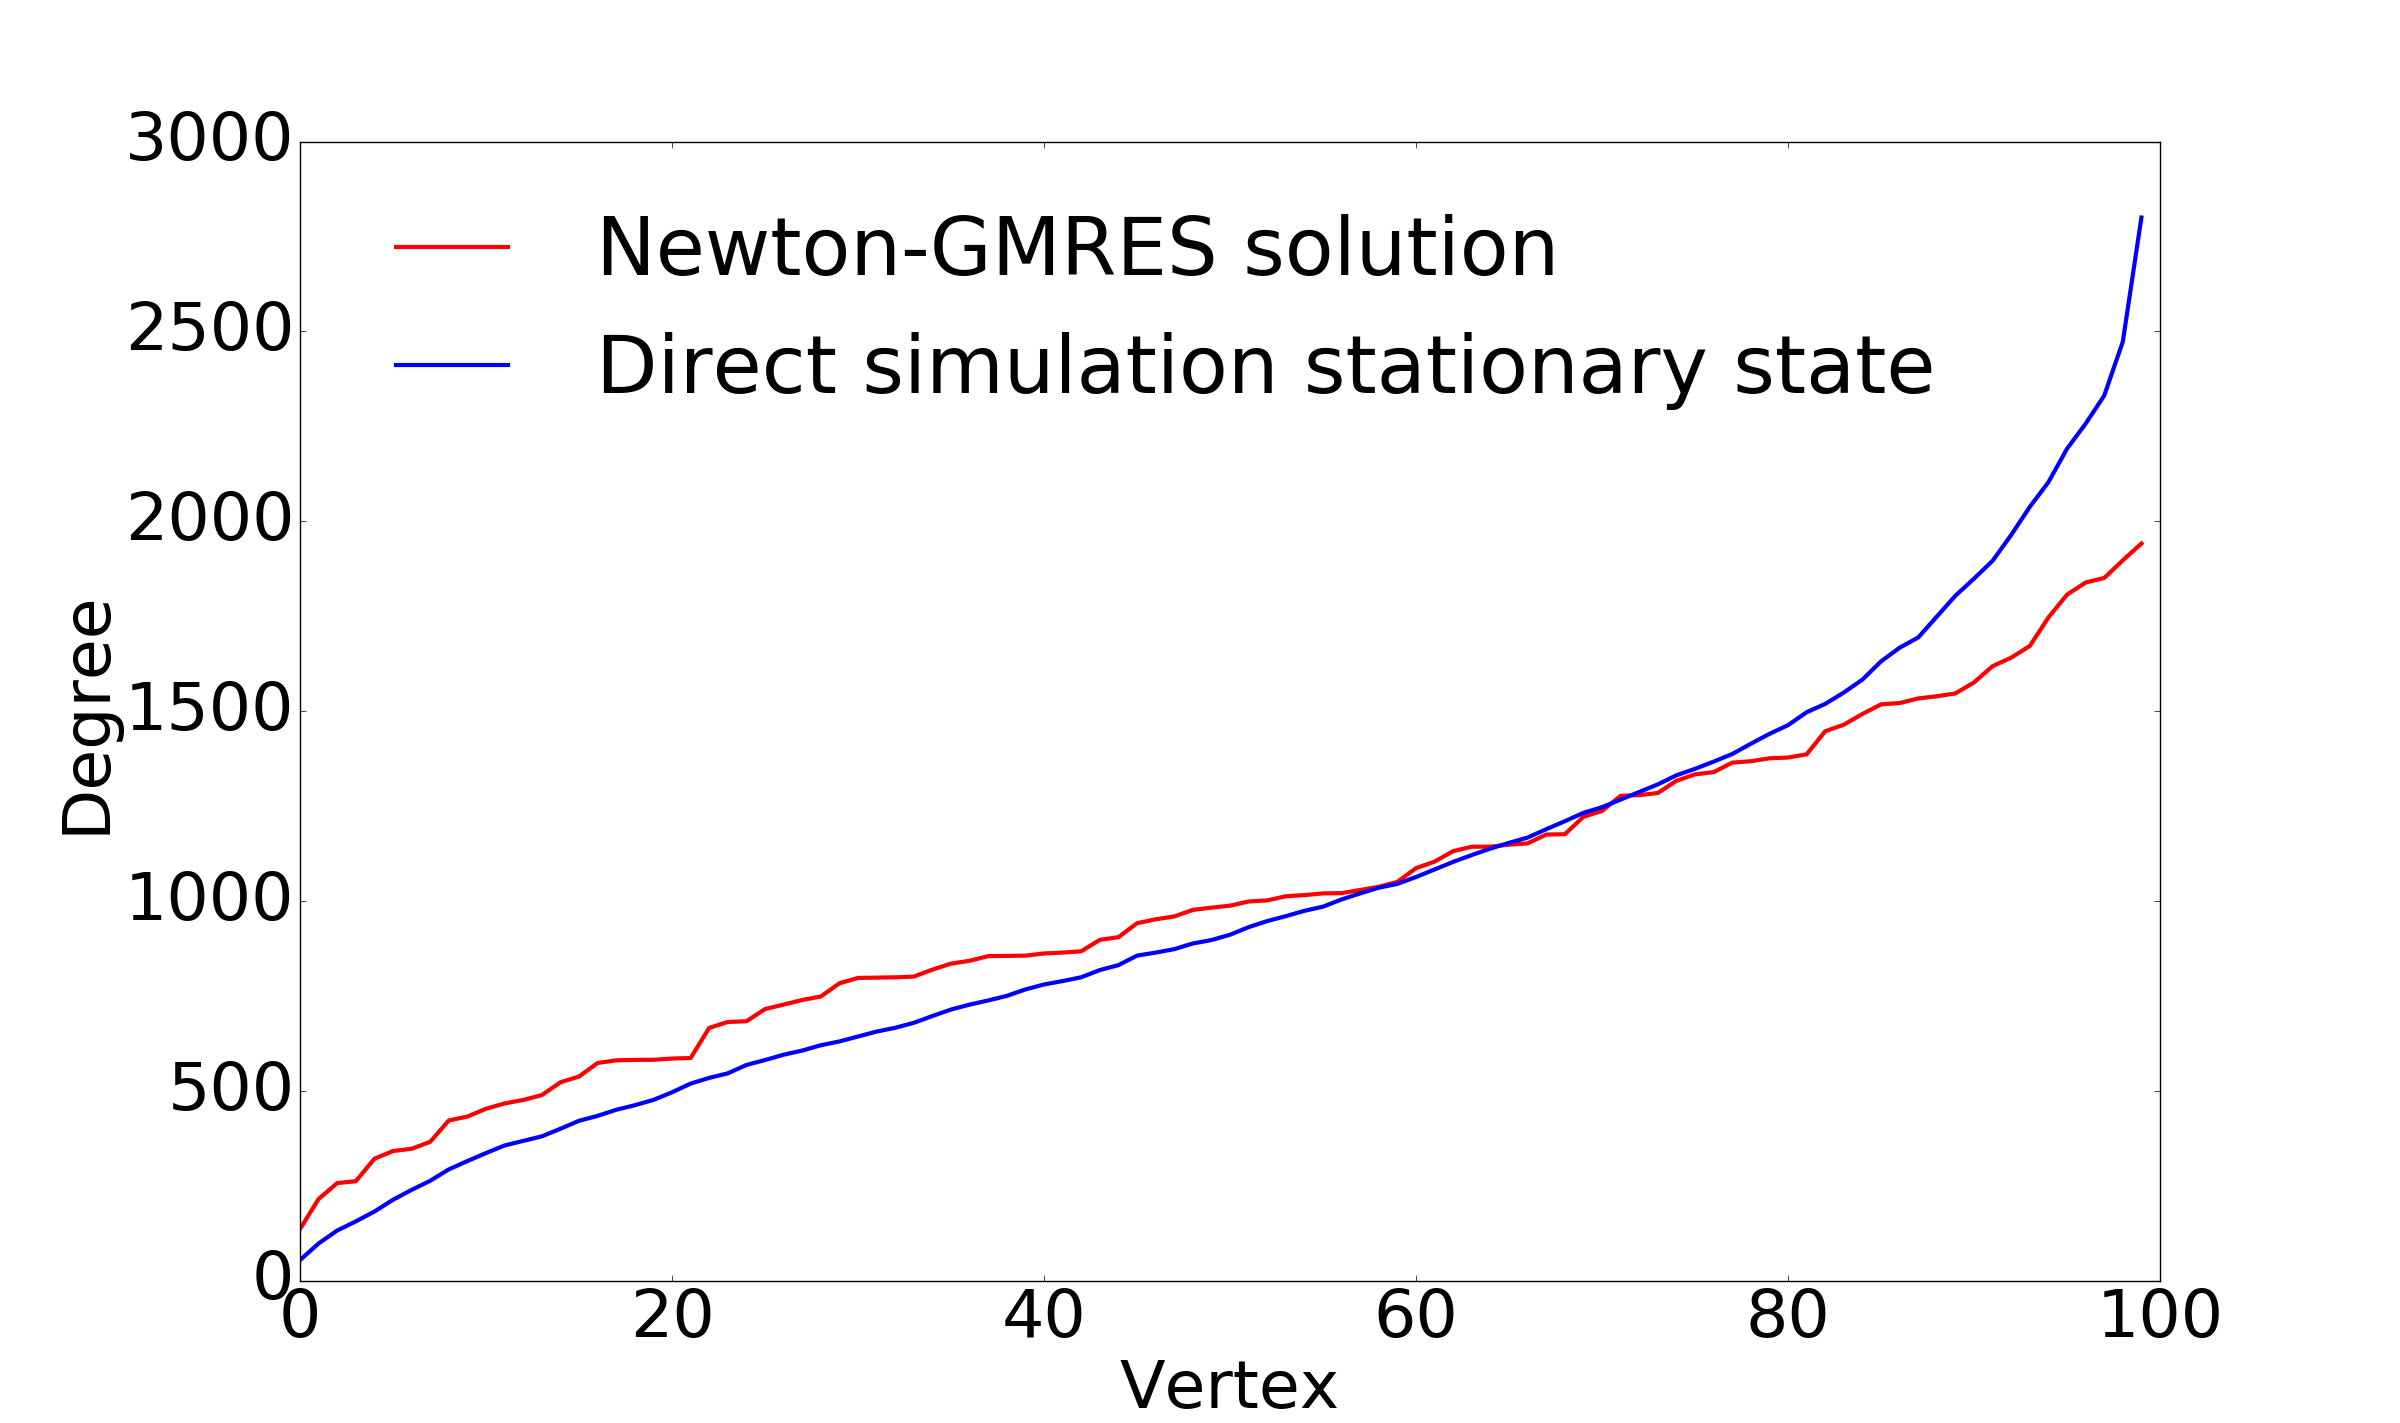
\includegraphics[width=\textwidth]{newton-comp}
      \subcaption{\label{fig:newton-comp}}
    \end{subfigure}%
    \caption[Coarse Newton-GMRES results]{Coarse Newton-GMRES results:
      (a) evolution of the error in the coarse Newton-GMRES iteration
      scheme; and (b) visual comparison of the algorithm's solution to
      the stationary state obtained from direct
      simulation. \label{fig:newton-results}}
  \end{figure}


  \section{Algorithmic coarse-graining}
  \label{sec:dr}
  Crucial to the above analysis was the determination of suitable
  coarse, system variables: it is the starting point of any equation
  free method.
  % 
  However, the discovery of such a low-dimensional description is
  highly non-trivial.
  % 
  Currently, as in this paper, they are ``discovered through informed
  experience'': through careful investigation of direct simulations,
  and knowledge of previous analytical results.
  % 
  Clearly, any process which could algorithmically guide this search
  based on only simulation data would be of great benefit to the
  modeling practitioner.
  % 
  We now illustrate two such algorithms: principal component analysis
  (PCA) and diffusion maps (DMAPS).
  % 
  First, we briefly discuss some aspects of the important issue of
  defining distances between networks, a prerequisite for any
  dimensionality-reduction technique.

  \subsection{On network distances}

  When applying dimensionality reduction techniques to a dataset, it
  is necessary to define a distance (or similarity) between each pair
  of data points.
  % 
  If these points are a set of vectors in $\mathbb{R}^n$ one has a
  number of metrics to choose from, the Euclidean distance being a
  common first option.
  % 
  Unfortunately, when individual points are not vectors but networks,
  the definition of a useful and computationally easily quantified
  metric becomes far more challenging.
  % 
  Examples such as the maximal common subgraph and edit distances,
  defined in \cite{bunke_graph_1998} and \cite{gao_survey_2010} define
  metrics on the space of graphs, but their computation is
  $NP\textnormal{-}hard$.
  % 
  Other computationally feasible approaches include comparing
  distributions of random walks on each graph
  \cite{vishwanathan_graph_2010}, calculating the so-called $n$-tangle
  density \cite{gallos_revealing_2014}, or calculating the edit
  distance
  with an approximation algorithm \cite{riesen_approximate_2009,zeng_comparing_2009}.

  The strategy used in the following computations, detailed in
  \cite{rajendran_analysis_2013} and \cite{xiao_structure-based_2008},
  enumerates the number of times a certain set of motifs (or
  subgraphs) appears in each network in the dataset.
  % 
  This maps each network to a vector in $\mathbb{R}^n$, and the
  Euclidean distance is subsequently used to quantify the similarity
  of two graphs.
  % 
  Due to computational restrictions, we chose here to only count the
  number of three- and four-vertex single-edge subgraphs contained in
  each network.
  % 
  As there are eight such motifs, shown in Fig. (\ref{fig:motifs}),
  this process $\gamma$ maps each graph to an eight-dimensional
  vector: $\gamma : G \rightarrow \mathbb{R}^8$.
  % 
  We applied this operation to a simplified version of each graph,
  wherein any multiple edges were reduced to a single edge.

  \begin{figure}
    \vspace{-5mm} \centering
    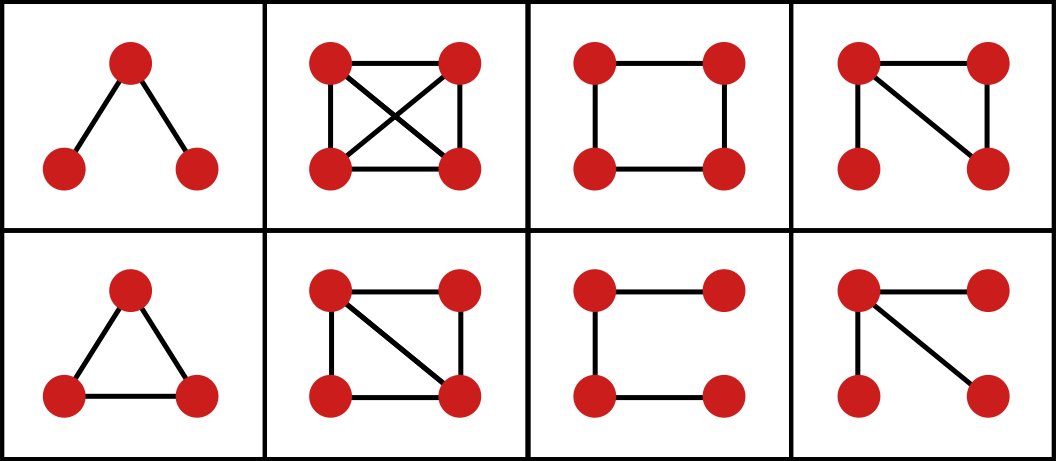
\includegraphics[width=\textwidth]{motifs}
    \caption[List of subgraphs used to embed multigraphs]{List of the
      single-edge subgraphs used to embed each network.  The number of
      times each appeared in the simplified input graph was
      calculated, mapping input graphs to
      $\mathbb{R}^8$. \label{fig:motifs}}
  \end{figure}

  \subsection{PCA\label{sec:pca}}
  

  PCA is used to embed data into linear subspaces that capture the
  directions along which the data varies most
  \cite{jolliffe_principal_2014}.
  % 
  Given some matrix $X \in \mathbb{R}^{n \times m}$ in which each of
  the $m$ column vectors $x_i$ represents a different collection of
  the $n$ system variables (i.e. a different data point), PCA computes
  a reduced set of $k<n$, orthogonal ``principal components''
  $z_i \in \mathbb{R}^n$ that constitute an optimal basis for the data
  in the sense that, among linear, $k$-dimensional embeddings,
  $w_i = Z^Tx_i$ captures the maximum possible variance in the
  dataset, where
  $Z = \begin{bmatrix} | & | & & | \\ z_1 & z_2 & \hdots & z_k \\ | &
    | & & | \end{bmatrix}$.
  % 
  This approach has found wide application, but can suffer from its
  inability to uncover simple \textit{nonlinear} relationships among
  the input variables.
  % 
  Indeed, many datasets will not ``just lie along some hyperplane''
  embedded in $\mathbb{R}^n$, but will rather lie on a low-dimensional
  nonlinear manifold throughout the space.

  Theoretical results in \cite{rath_time_2012} state that, for a given
  network size $n$, the final stationary state depends only on the
  number of edges present $m$ and the model parameter $\kappa$.
  % 
  To assess both the validity of our graph embedding technique and the
  usefulness of PCA in the context of complex networks, we generated a
  dataset of stationary states over a range of $m \in [50, 5000]$ and
  $\log(\kappa) \in [0, 2]$ values by directly running the model over
  $2n^3$ steps ($N=30$ values of each parameter were taken, for a
  total of $900$ networks).
  % 
  We fixed the network size to $n=50$ vertices.
  % 
  Each resulting graph $G(m_i, \kappa_j) = G_{ij}$ was then embedded
  into $\mathbb{R}^8$ by counting the number of times each of the
  subgraphs shown in Fig. (\ref{fig:motifs}) appeared in the network.
  % 
  Thus $\gamma(G_{ij}) = v_{ij} \in \mathbb{R}^8$.
  % 
  We then proceeded to perform a principal component analysis on this
  collection of vectors $\{v_{ij}\}_{i,j=1}^N$.
  % 
  Interestingly, the first two principal components $z_1$ and $z_2$
  succeeded in uncovering a two-dimensional embedding of the dataset
  corresponding to the two underlying parameters $m$ and $\kappa$, as
  shown in Fig. (\ref{fig:pca}) in which the data is projected on the
  plane spanned by these two vectors.
  % 
  This suggests that, given some final network state $G(m, \kappa)$,
  by projecting its embedding onto these first two principal
  components one could obtain a reasonable approximation of the hidden
  parameter $\kappa$.

  \begin{figure}
    \vspace{-5mm} \centering
    \begin{subfigure}{0.49\textwidth}
      \centering
      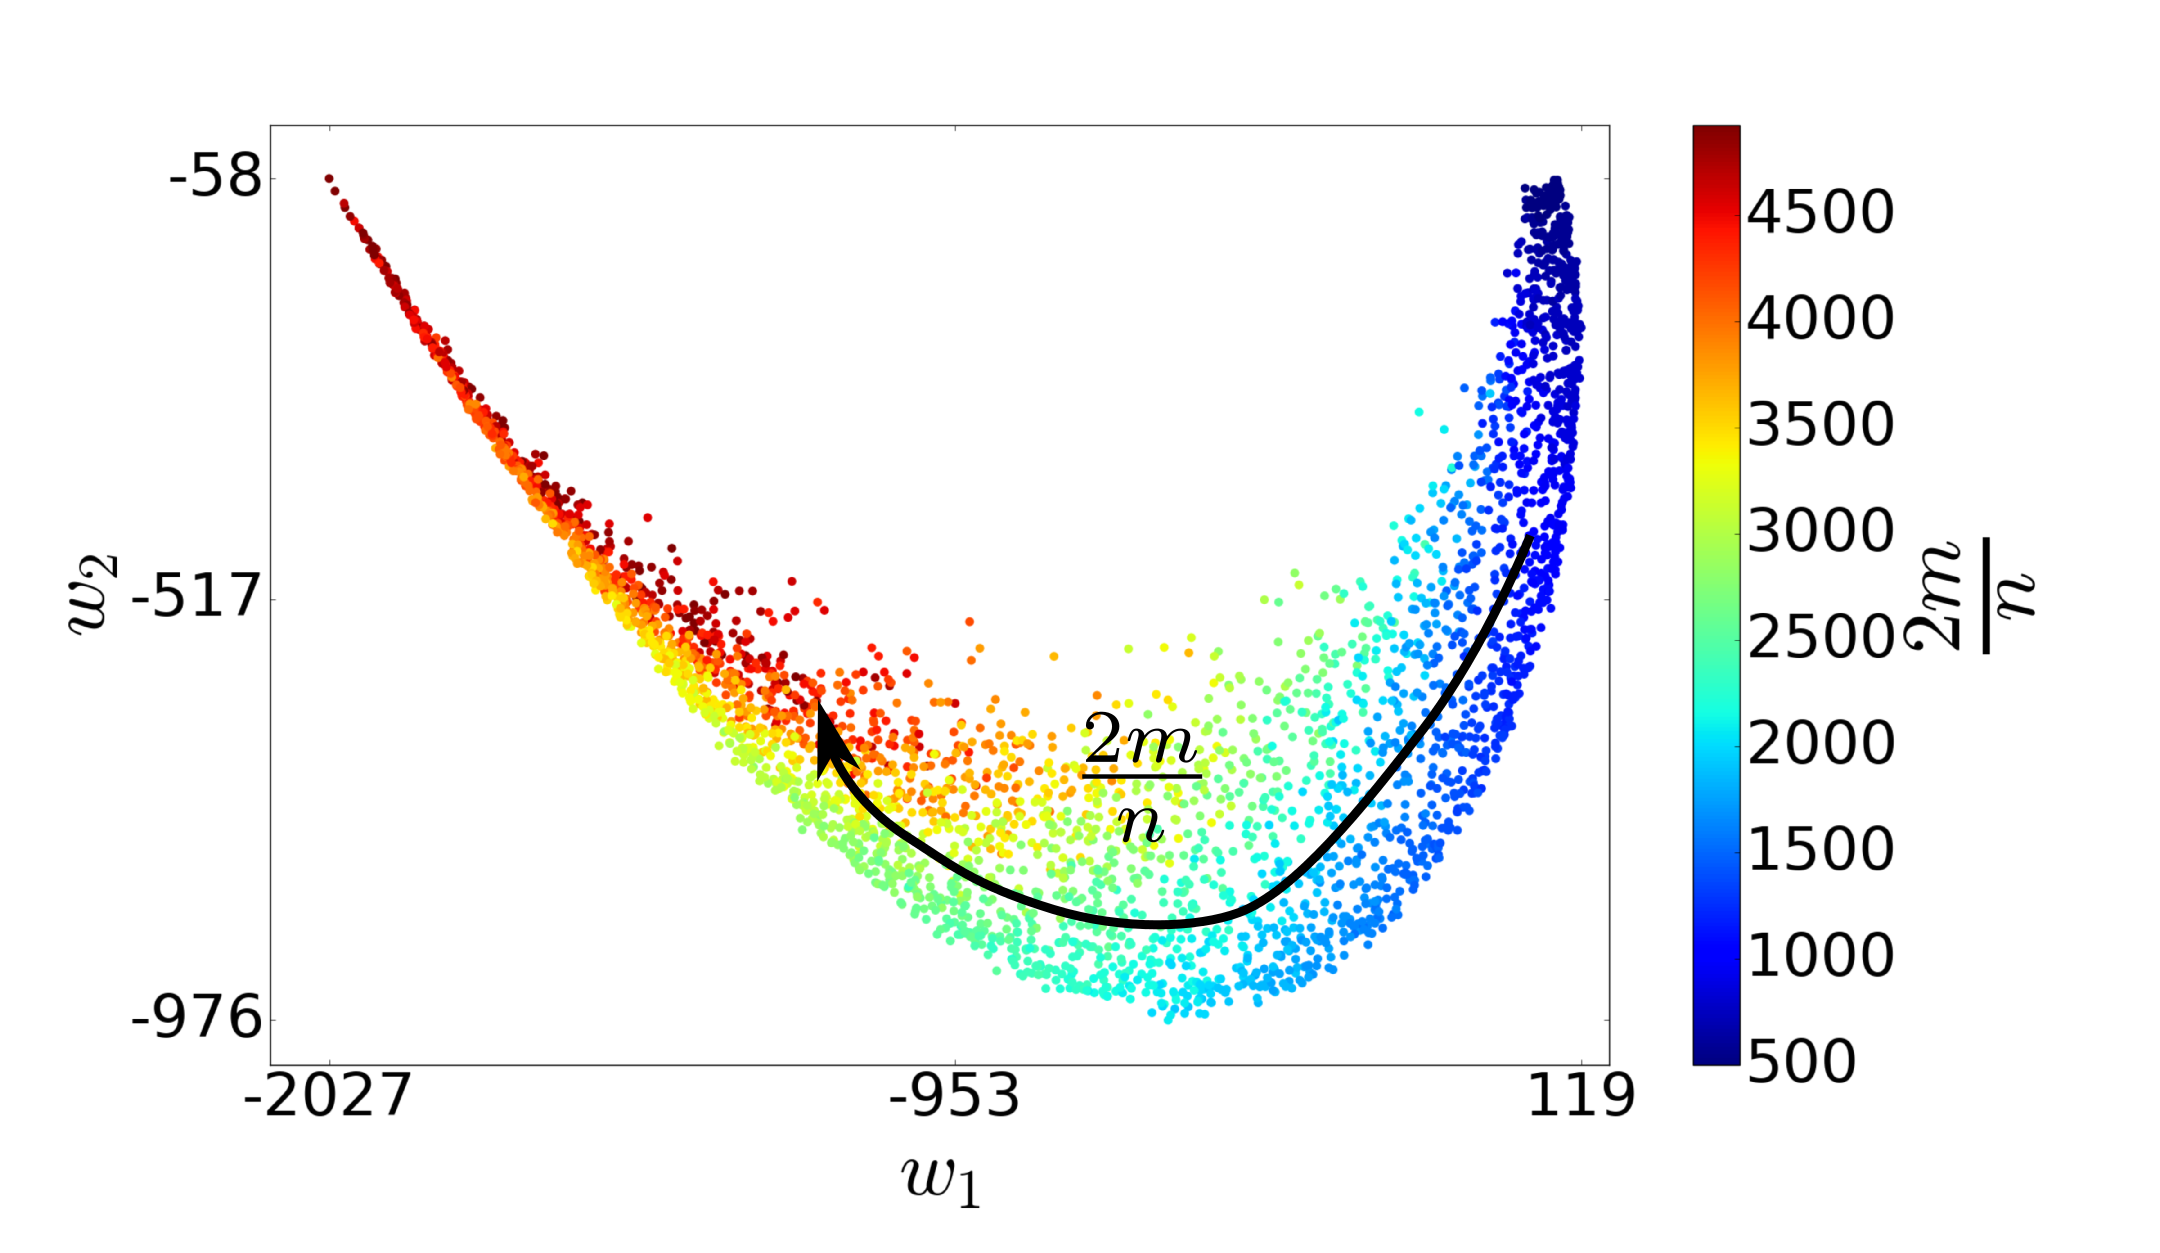
\includegraphics[width=\textwidth]{pca-2d-rho-a}
      \subcaption{\label{fig:pca-rho}}
    \end{subfigure} %
    \begin{subfigure}{0.49\textwidth}
      \centering
      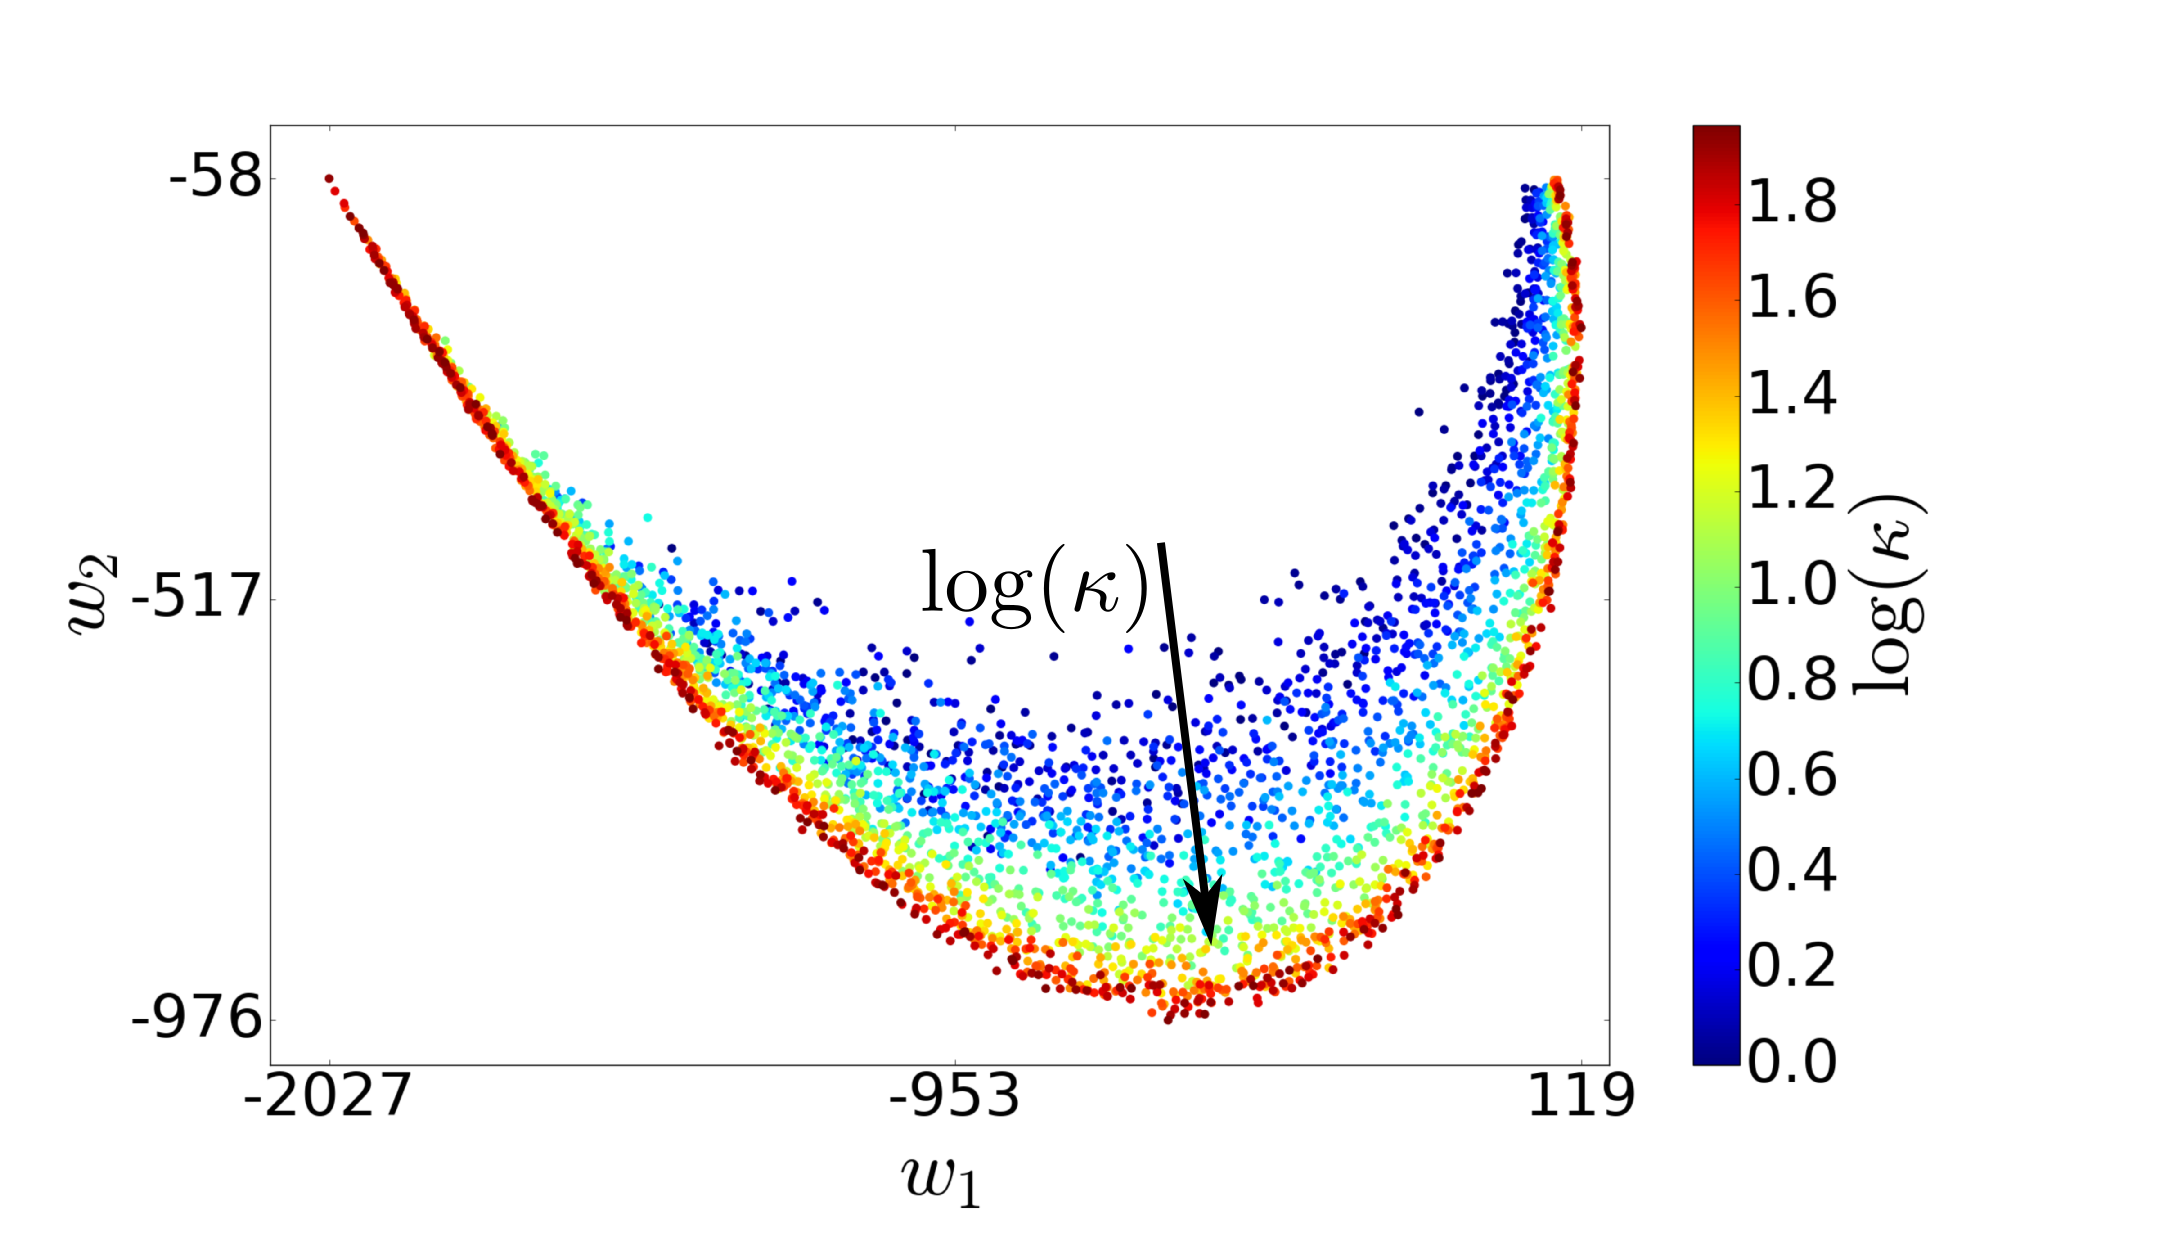
\includegraphics[width=\textwidth]{pca-2d-kappa-a}
      \subcaption{\label{fig:pca-kappa}}
    \end{subfigure}%
    \caption[Principal component analysis of motif-based
    embeddings]{PCA of motif-based embeddings: (a) coloring the
      two-dimensional PCA embedding with $\rho$ and (b) coloring the
      two-dimensional PCA embedding with $\kappa$. \label{fig:pca}}
  \end{figure}

  \subsection{Diffusion Maps}

  Unlike PCA, DMAPS uncovers parameterizations of nonlinear manifolds
  hidden in the data.
  % 
  This is achieved by solving for the discrete equivalent of the
  eigenfunctions and eigenvalues of the Laplace-Beltrami operator over
  the manifold, which amounts to calculating leading
  eigenvector/eigenvalue pairs of a Markov matrix $A$ describing a
  diffusion process on the dataset.
  % 
  As the eigenfunctions of the Laplace-Beltrami operator provide
  parameterizations of the underlying domain, the output eigenvectors
  $\Phi_i$ from DMAPS similarly reveal and parameterize any hidden
  nonlinear structure in the input dataset. The $k$-dimensional DMAP
  of point $x_i$ is given by

  \begin{align*}
    \Psi(x_i; t) = \begin{bmatrix} \lambda_1^t \Phi_1(i) \\ \lambda_2^t
      \Phi_2(i) \\ \vdots \\
      \lambda_k^t \Phi_k(i) \end{bmatrix}
  \end{align*}

  \noindent where $\lambda_i$ is the $i^{th}$ eigenvalue of the Markov
  matrix $A$, $\Phi_i(j)$ the $j^{th}$ entry of eigenvector $i$, and
  the parameter $t$ allows one to probe multiscale features in the
  dataset. See \cite{coifman_diffusion_2006,nadler_diffusion_2006} for
  further details.

  First we applied DMAPS to the dataset described in
  Sec. (\ref{sec:pca}).
  % 
  Given the apparent success of PCA in this setting, one would expect
  DMAPS to also uncover the two-dimensional embedding corresponding to
  different values of $m$ and $\kappa$.
  % 
  Fig. (\ref{fig:dmaps-rk}) shows that this is indeed the case: using
  $\Phi_1$ and $\Phi_4$ to embed the graphs produces a two-dimensional
  surface along which both $\rho$ and $\kappa$ vary independently.

  Additionally, we were interested in embeddings of different model
  trajectories.
  % 
  This dataset was generated by sampling two different model
  simulations as they evolved ($N=2000$ points were sampled from each
  trajectory).
  % 
  The parameters $n$, $m$ and $\kappa$ were held constant at $200$,
  $20100$ and $1.0$ respectively, but one graph was initialized as an
  Erd\H{o}s-R\'{e}nyi random graph (Fig. (\ref{fig:erdos-init})),
  while the other was initialized as a ``lopsided'' graph
  (Fig. (\ref{fig:lopsided-init})).
  % 
  Every $500$ steps the graph would be recorded till $N$ snapshots
  were taken of each trajectory, for a total of $1000000$ steps.
  % 
  Letting $G_e(t)$ refer to the Erd\H{o}s-R\'{e}nyi-initialized system
  at step $t$, and $G_l(t)$ the lopsided-initialized system, the
  embedding $\gamma$ was used to create points
  $\gamma(G_e(t)) = v_e(t) \in \mathbb{R}^8$ and
  similarly $\gamma(G_l(t)) = v_l(t) \in \mathbb{R}^8$.

  DMAPS was then applied to this set of $2N$ points, and the
  three-dimensional embedding using $\Phi_1$, $\Phi_2$ and $\Phi_3$ is
  shown in Fig. (\ref{fig:dmaps-results}).
  % 
  At first, the two trajectories are mapped to distant regions in
  $\mathbb{R}^3$ due to their different initial conditions.
  % 
  They evolve along different ``regions'' of the embedding, taking two
  distinct trajectories on their approach to the stationary state.
  % 
  Eventually, their embeddings meet as they arrive at this final,
  shared state, each asymptotically along opposite sides of the
  slowest eigenvector of the linearization of the steady state.
  % 
  DMAPS thus proves useful in elucidating both geometric and dynamic
  features of the system as shown in Figs. (\ref{fig:dmaps-rk}) and (\ref{fig:dmaps-results}).

  We see that both PCA and DMAPS, when combined with a suitable
  embedding of each graph, can help uncover useful information
  pertaining to the underlying dimensionality of the problem dynamics.


  \begin{figure}
    \vspace{-5mm} \centering
    \begin{subfigure}{0.49\textwidth}
      \centering
      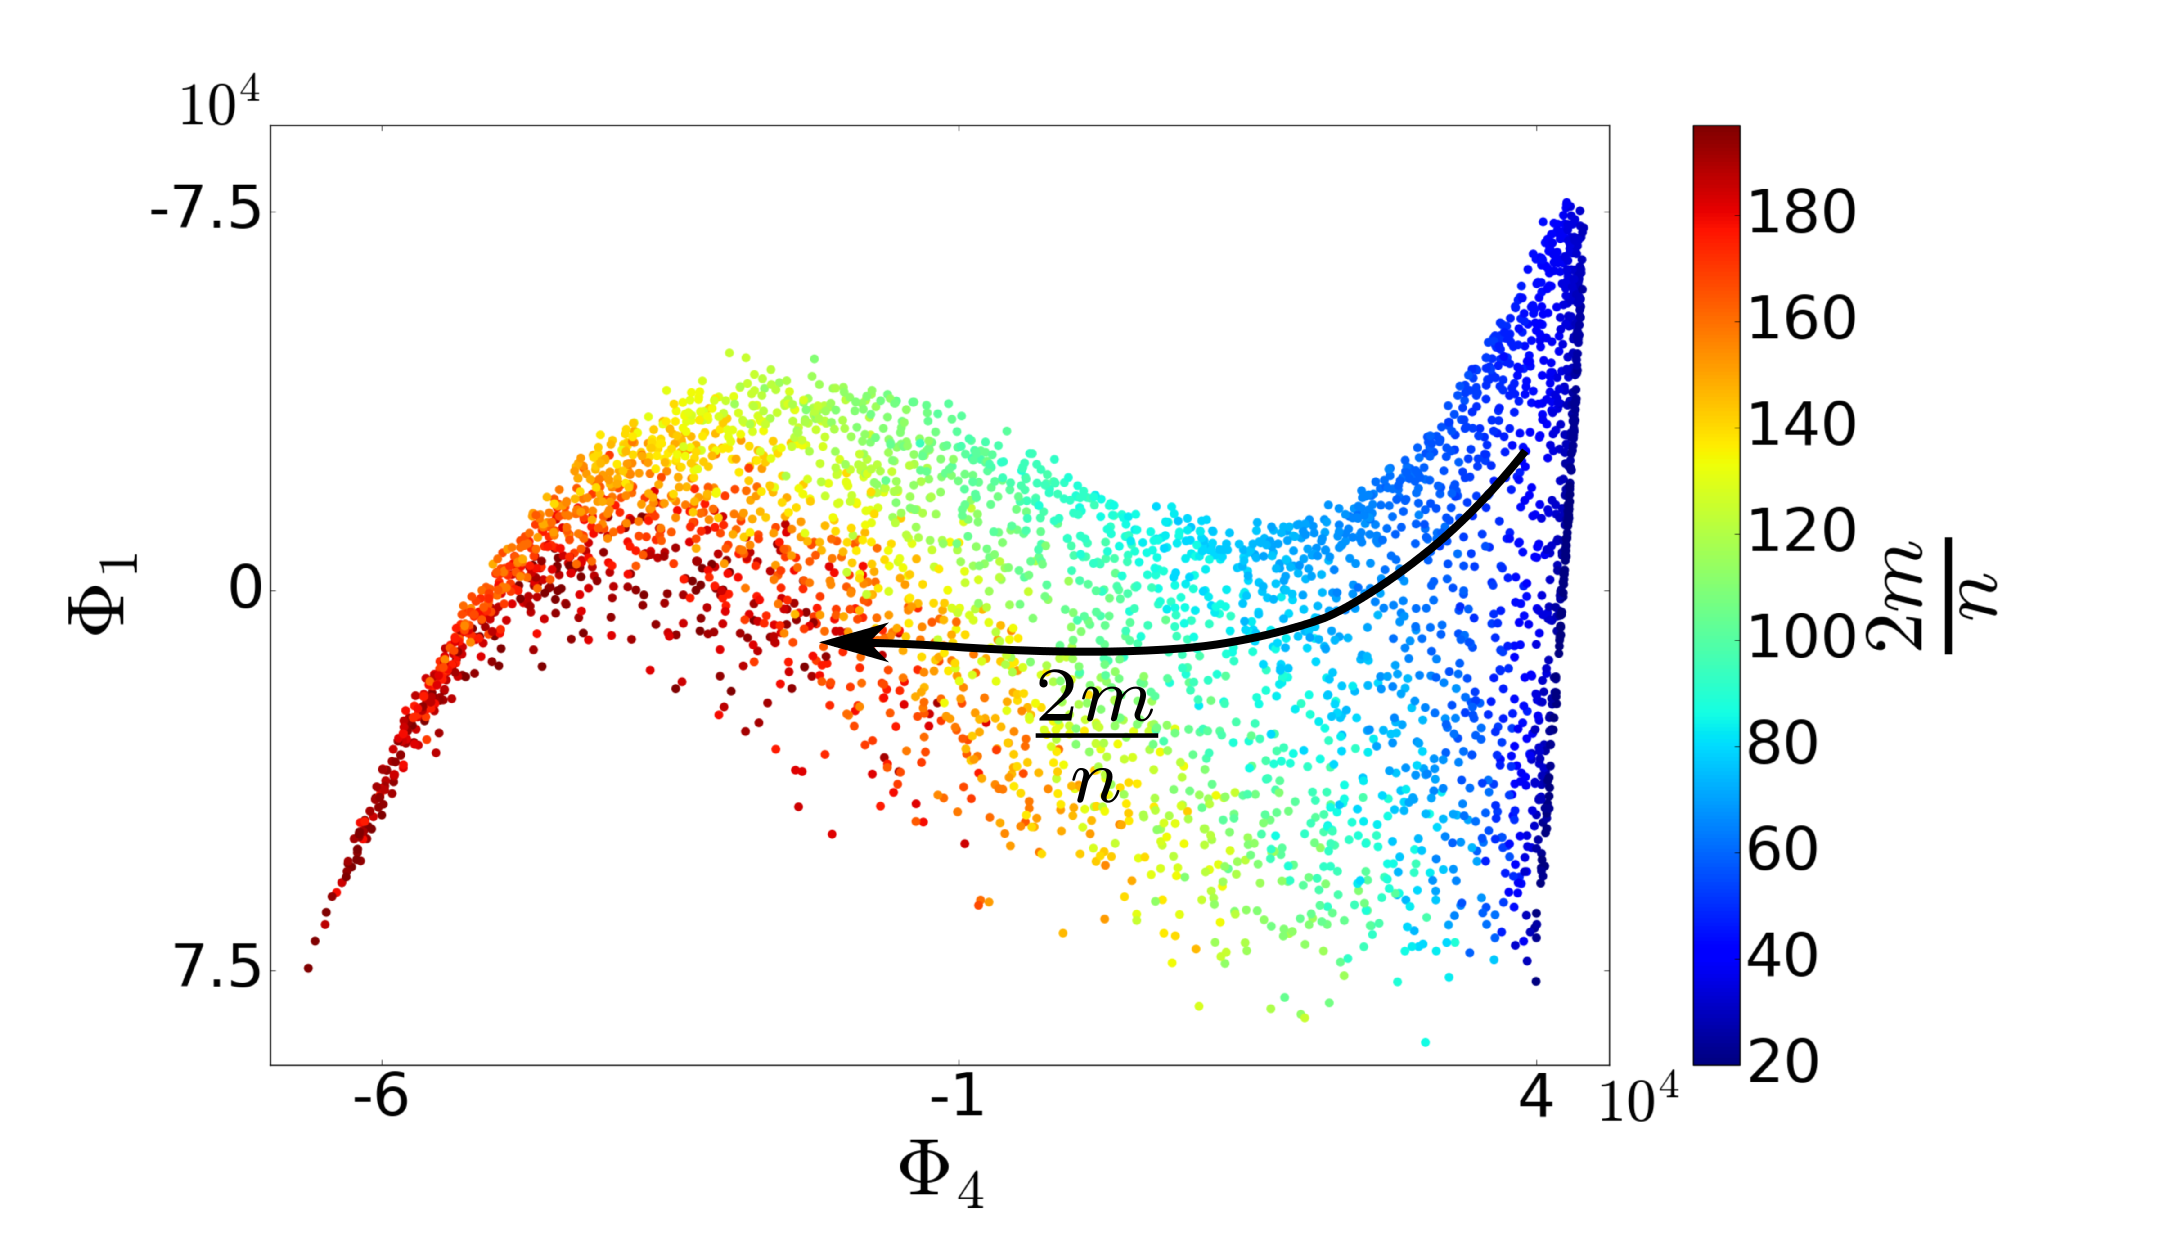
\includegraphics[width=\textwidth]{dmaps-2d-rho-a}
      \subcaption{\label{fig:dmaps-rho}}
    \end{subfigure} %
    \begin{subfigure}{0.49\textwidth}
      \centering
      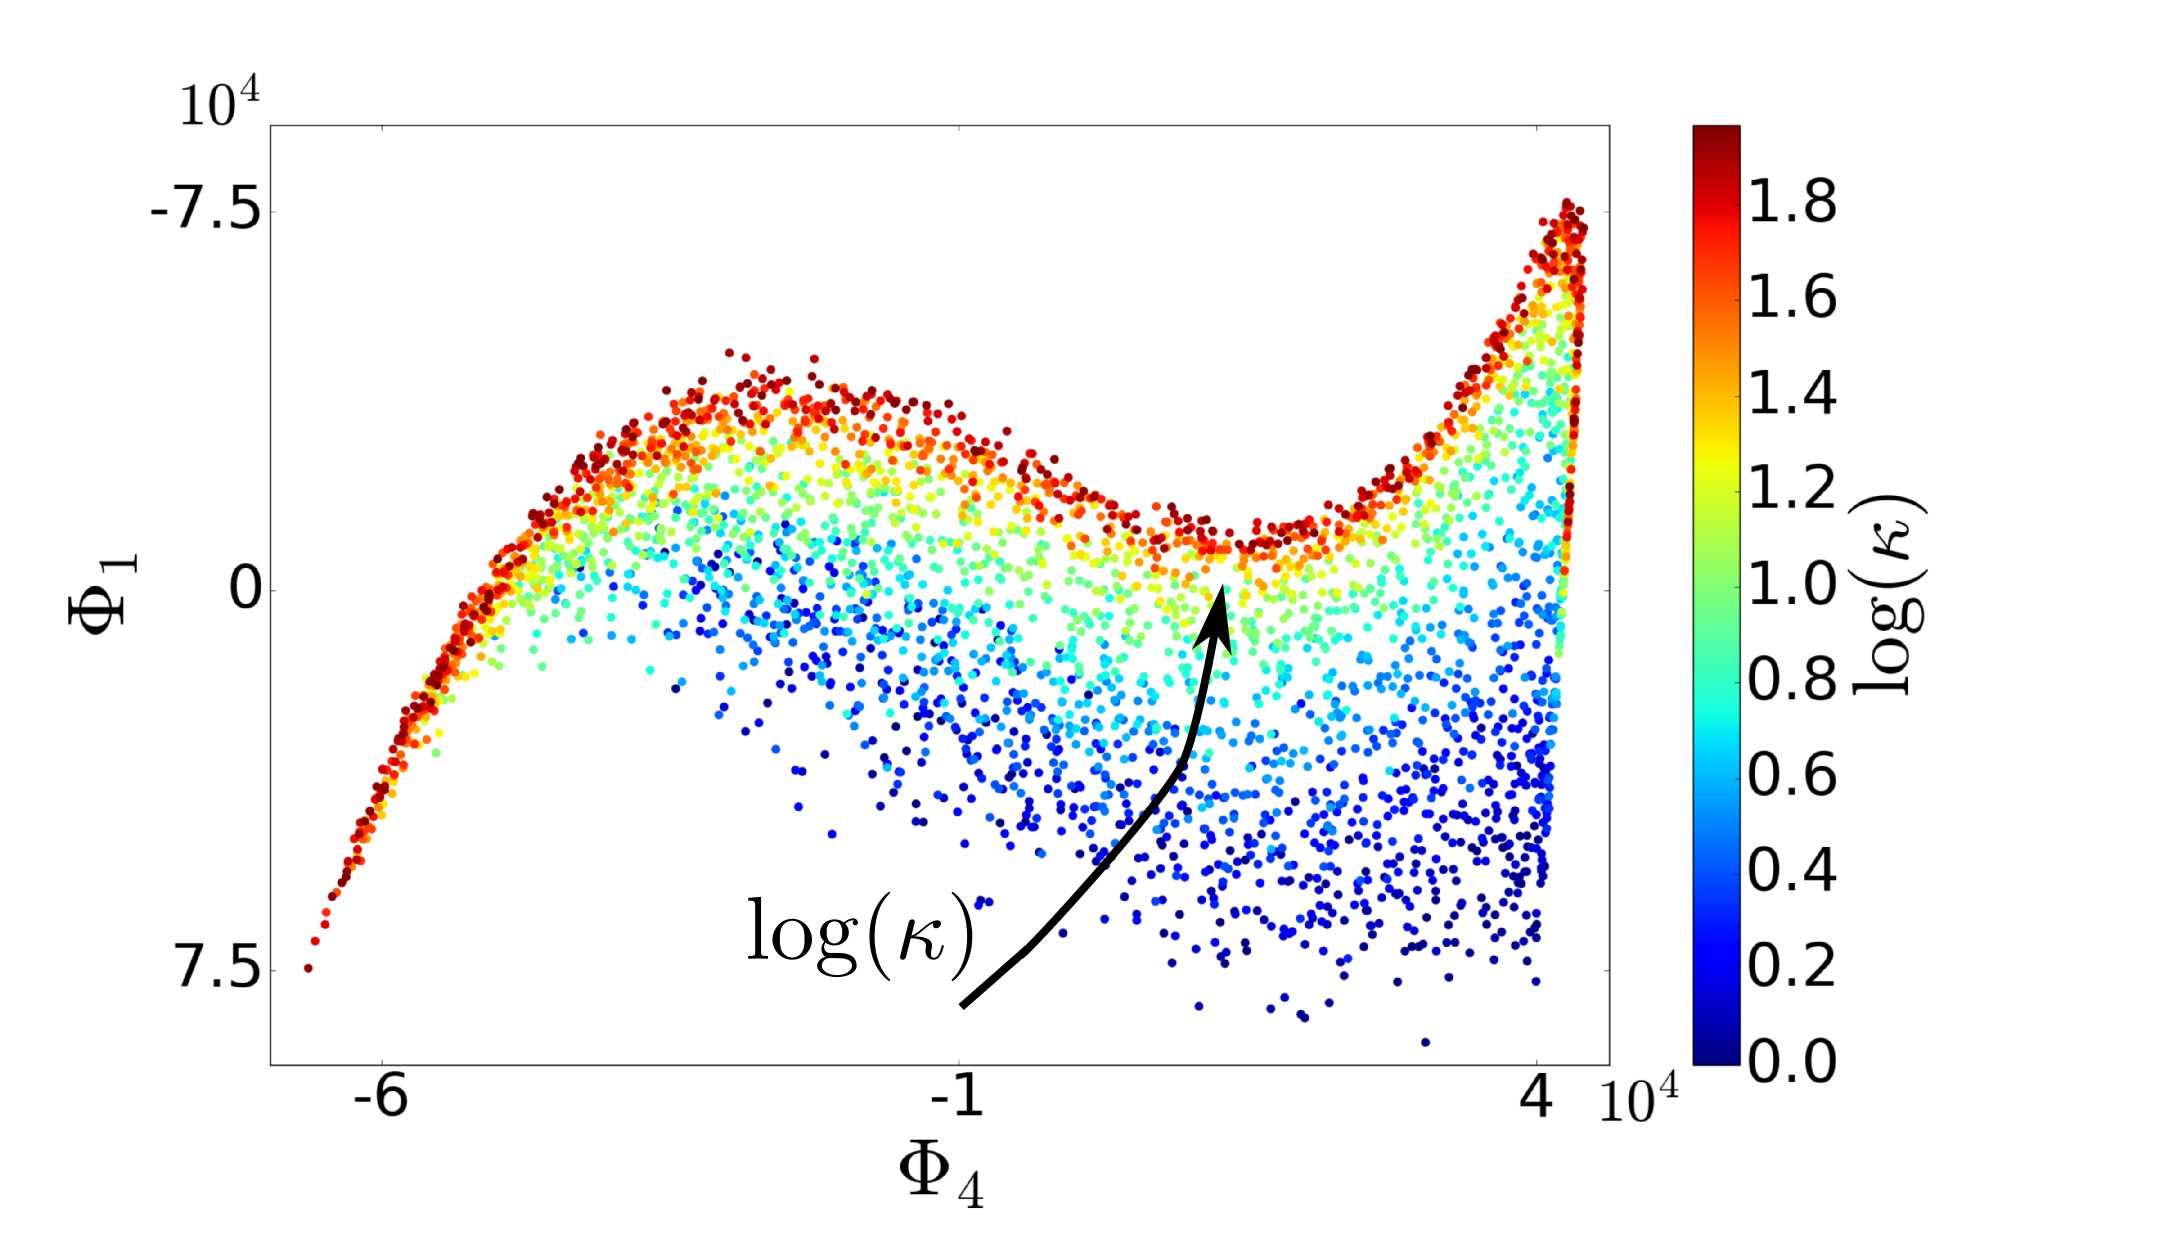
\includegraphics[width=\textwidth]{dmaps-2d-kappa-a}
      \subcaption{\label{fig:dmaps-kappa}}
    \end{subfigure}%
    \caption[DMAP of motif-based embeddings when system parameters are
    varied]{DMAP of motif-based embeddings from a collection of
      simulations run at different parameter values: (a) coloring the
      two-dimensional DMAPS embedding with $\rho$ and (b) coloring the
      two-dimensional DMAPS embedding with $\kappa$. As with PCA,
      DMAPS uncovered the parameters governing the stationary state,
      known from \cite{rath_time_2012} \label{fig:dmaps-rk}}
  \end{figure}

  \begin{figure}
    \vspace{-5mm} \centering
    \begin{subfigure}{0.49\textwidth}
      \centering
      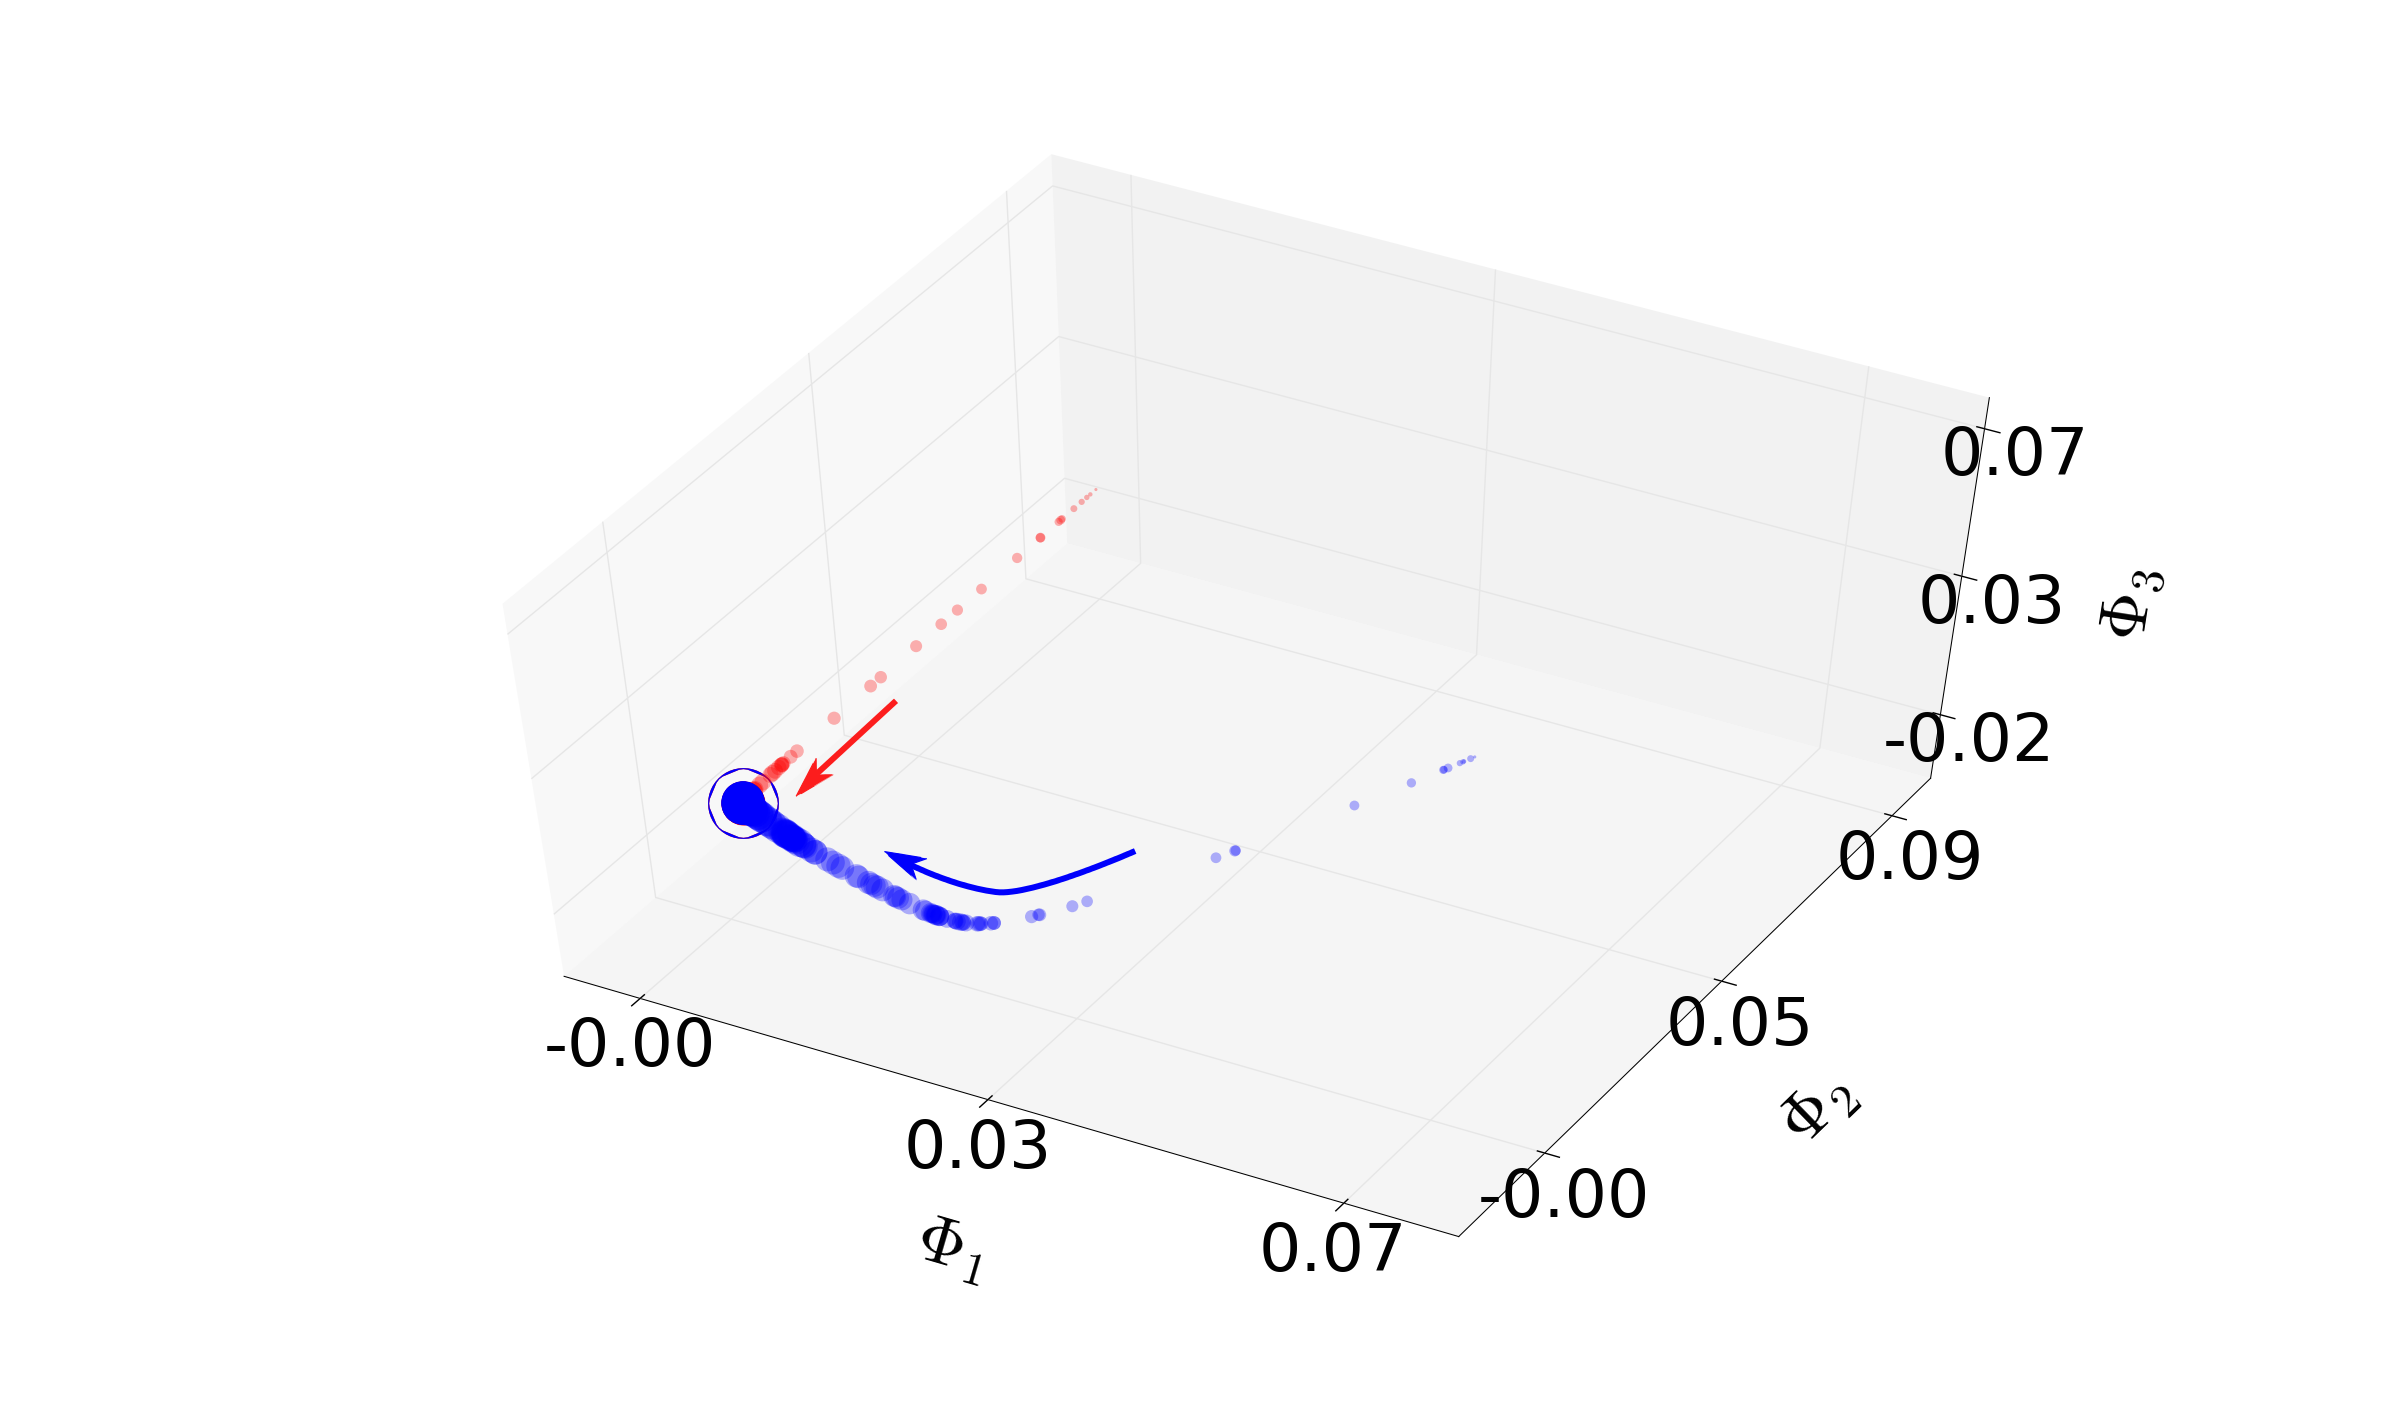
\includegraphics[width=\textwidth]{dmaps-3d-convergence-a}
      \subcaption{\label{fig:dmaps-results-regular}}
    \end{subfigure} %
    \begin{subfigure}{0.49\textwidth}
      \centering
      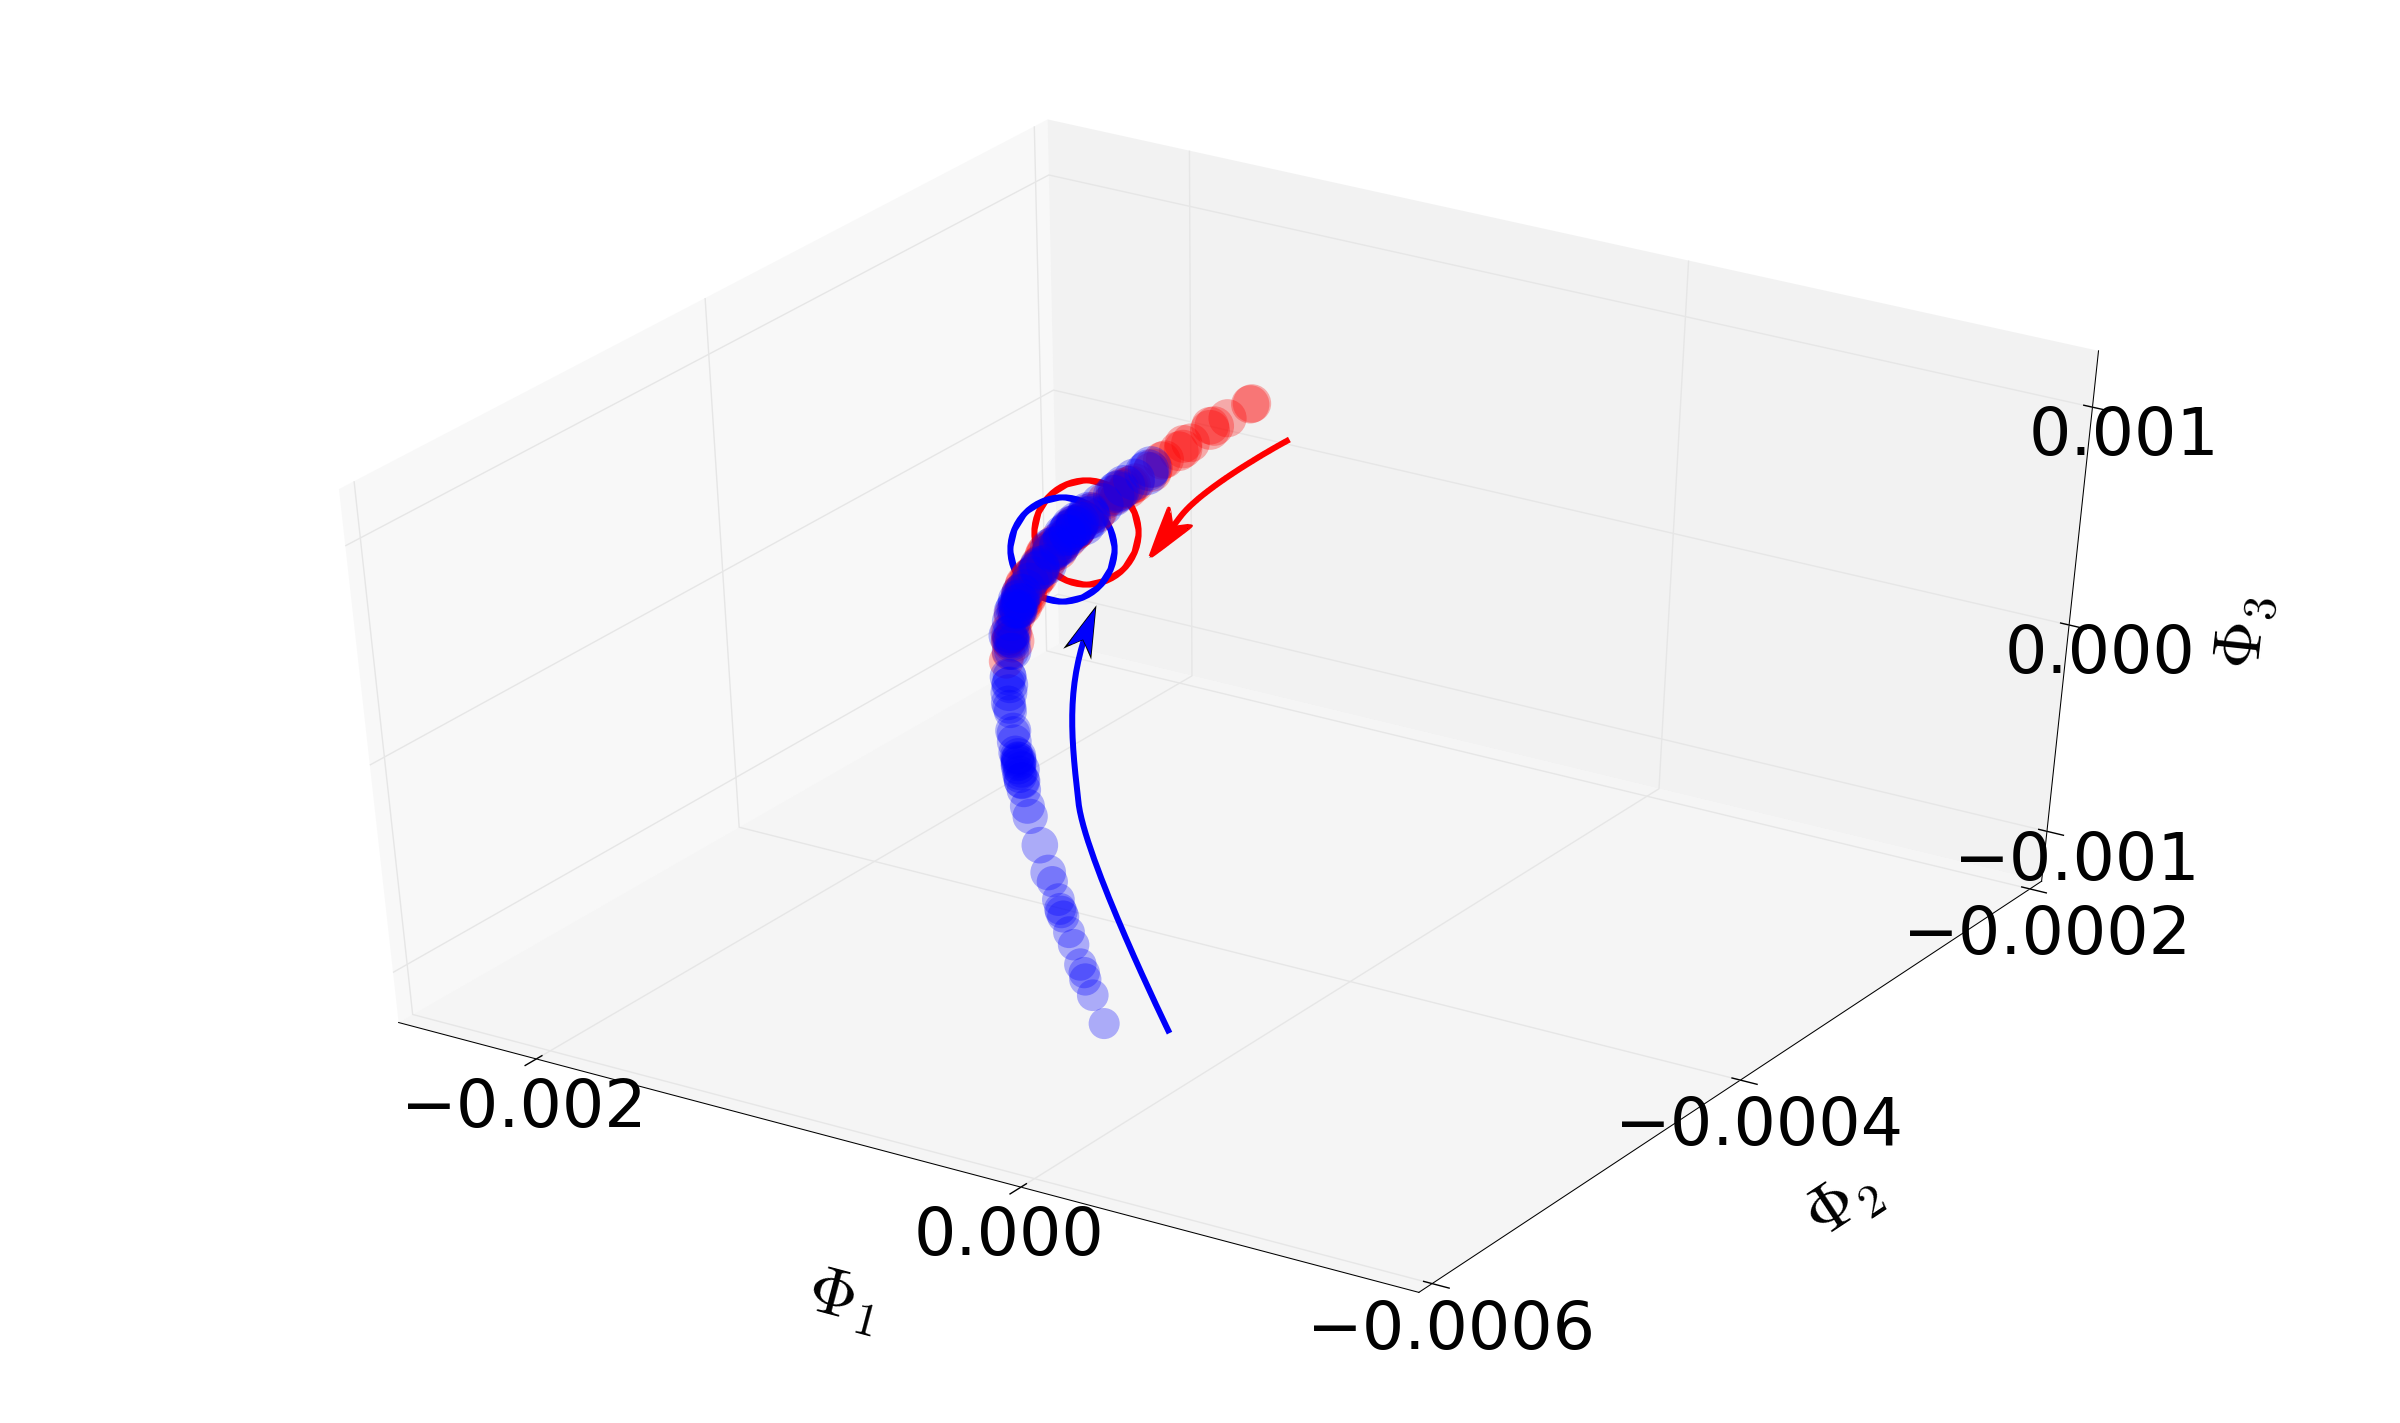
\includegraphics[width=\textwidth]{dmaps-3d-convergence-zoom-a}
      \subcaption{\label{fig:dmaps-results-zoom}}
    \end{subfigure}%
    \caption[DMAP of motif-based embeddings when two trajectories are
    sampled]{DMAP of motif-based embeddings from two separate
      simulation trajectories: (a) embedding of two trajectories
      starting from different initial conditions. While the
      trajectories are initially mapped to separate regions of
      ``embedding space'', they eventually evolve to the same coarse
      stationary state.  Final states are circled, and point size
      grows as more steps are taken in each trajectory.  (b) Enlarged
      view of the final points in the previous plot, revealing the
      approach to a similar final state along opposite sides of the
      slowest eigenvector of its linearization.  Here, the average of
      the final fifty points is circled. Due to the stochastic nature
      of the system, the final embeddings mildly fluctuate randomly
      about the shared stationary state. \label{fig:dmaps-results}}
  \end{figure}

  \section{Conclusion}

  The equation free framework was successfully applied to the
  edge-conservative preferential attachment model, accelerating
  simulations through CPI and locating stationary states through
  coarse Newton-GMRES. This indicates potential avenues for improving
  simulation times of other complex network models, such as those
  found in epidemiology.
  % 
  Additionally, an underlying two-dimensional description was
  uncovered via PCA and DMAPS. These automated methods of
  dimensionality-reduction are quite general, and can in principle be
  applied in a wide range of network settings to probe hidden
  low-dimensional structure. For an application in the setting of
  labeled nodes, see ({\cite{kattis_modeling_2016}}).

  However, an open area of investigation is the interpretation of the
  output from the PCA and DMAPS techniques.
  % 
  As a linear map, PCA retains a clear relationship between its input
  and output, but is less effective when data lie on highly nonlinear
  manifolds.
  % 
  DMAPS may perform better the task of dimensionality reduction, but
  it is unclear how the embedding coordinates relate to physical
  features of the sampled networks.
  % 
  While this approach opens several promising avenues in
  coarse-graining complex network dynamics, it also reveals two
  ``bottlenecks'' for the process: (a) the selection of informative
  and practically computable graph distance metrics, necessary in the
  discovery of good coarse variables; and (b) the construction of
  network realizations consistent with (conditioned on) specific
  values of collective observables.
  % 
  Both items are, and we expect will continue being, the subject of
  intense investigation by many research groups, including ours.

\chapter{Identifying significant parameters combinations in complex
  models \label{ch:params}}


% \begin{abstract}
%   Detailed dynamical models can often be summarized in terms of only
%   a few components, reducing complexity and making exploration
%   easier and more insightful.  Pen-and-paper reduction is tedious
%   and impractical for most models, however it has the added benefit
%   of identifying parameter combinations that matter most.  Recently
%   developed frameworks computerizing model reduction leave the dual
%   aspect of effective parameter identification unaddressed,
%   relegating parameter space exploration subject to ineffective
%   sampling strategies.  Here, we lay the foundation for systematic
%   parameter reduction, rooting it in the same nonlinear data mining
%   techniques that powered model reduction in our earlier
%   equation-free framework.  Our ambition is to extend the
%   data-driven determination of effective variables by integrating
%   into it the discovery of effective model parameters.  This will
%   accelerate both dynamical simulations and parametric explorations,
%   allowing us to efficiently map out the behavior of complex models.

% \end{abstract}

The past decades have seen a steady fall in the cost of computation,
enabling systems to be studied using increasingly complex models.
Perceptron networks in the 1960's contained thousands of hidden units
\cite{nagy_neural_1991}, while modern neural nets are comprised of
billions \cite{hsu_biggest_2015}. Molecular dynamics simulations in
1957 entailed tens of hard-sphere particles \cite{alder_phase_1957};
today we model entire proteins and their folding dynamics
\cite{piana_atomic-level_2013}. And Lorenz's three-dimensional system
of equations describing atmospheric convection in 1963
\cite{lorenz_deterministic_1963} led to modern large eddy simulations
run across multiple computing clusters \cite{ghosal_dynamic_1995}. In
all cases, the improvement in precision afforded by increased model
complexity is matched by an increased number of model parameters.

Highly parameterized models may aid accuracy, but the effect of each
individual parameter on the overall model output is often difficult to
ascertain. Indeed, it has been well-document that a wide array of
systems contain particular hidden parameters that appear to have no
influence on the model's predictions
\cite{gutenkunst_extracting_2007}. These have been termed ``sloppy
parameters'', and their presence seems ubiquitous in contemporary
systems \cite{gutenkunst_universally_2007}. This is problematic as not
only do sloppy parameters obfuscate the inputs that actually
matter, but they also lead to slow convergence of model-fitting
algorithms \cite{transtrum_geometry_2011}.

Several approaches have been suggested to combat this
over-parameterization. Some, such as the Manifold Boundary
Approximation Method ultimately rely on deriving by hand a reduced
model \cite{transtrum_model_2014}. Others, such as Active Subspaces
make assumptions about linearity that may not hold in practical
settings \cite{constantine_active_2015}. Here, we present a
data-driven approach to parameter reduction that is flexible enough to
handle nonlinear systems. This is accomplished through Diffusion Maps
(DMAPS), an established manifold learning technique that we adapt to
this context \cite{coifman_diffusion_2006}. We begin with a
description of our formulation of the problem, and then present a
simple example that clearly shows the consequences of sloppiness,
while also providing some intuition as to how it emerges.

Our overall approach is motivated by the work in
\cite{transtrum_geometry_2011}. We consider a model to consist of a
vector of parameters $\theta \in \mathbb{R}^k$ and a function mapping
these inputs to a model response (or model output) in $\mathbb{R}^n$,
$f: \mathbb{R}^k \rightarrow \mathbb{R}^n$. Sloppiness would reveal
itself as regions of parameter space, $\Omega_S \in \mathbb{R}^k$ in
which the model reponse remains nearly constant:
$f(\theta_i) \approx f(\theta_j)\; \theta_i, \theta_j \in
\Omega_S$. We will also denote distances in parameter space as
$\delta(\theta_i, \theta_j) = \| f(\theta_i) - f(\theta_j)\|_2$, that
is, the Euclidean distance between the resulting model responses. To
provide a concrete example, consider a model with parameters $p_1$ and
$p_2$, and model output
$f(p_1, p_2) = (p_1 p_2 , \ln(p_1) + \ln(p_2) , (p_1 p_2)^2)$. Then
$\theta = (p_1, p_2) \in \mathbb{R}^2$ and $f: \R^2 \rightarrow
\R^3$. It is clear from the expression for $f$ that the model response
depends only on the overall product $p_1 p_2$, and not on $p_1$ and
$p_2$ independently. To make it explicit, set $p_{eff} = p_1 p_2$ and
rewrite $f$ as $(p_{eff}, \ln(p_{eff}), p_{eff}^2)$. Thus, although we
have chosen to include both $p_1$ and $p_2$ as independent parameters
in our original model, only the value of $p_{eff}$ is significant. Also note
that if we only had access to a black-box function evaluator, it would
be non-trivial to determine the existence of $p_{eff}$ at all.

This model is illustrated in Figure~\ref{fig:non-id}, where curves of
constant color denote sets of constant model response. If we had
sampled data corresponding to true parameter values of
$p_1^* = p_2^* = 1$, Figure~\ref{fig:non-id} also reveals how
sloppiness affects optimization routines trying to fit such
data. Convergence is permitted along entire bands of parameter space
instead of at a single point. The inset shows $\delta$-contours of a
slightly perturbed system in which both $p_1$ and $p_2$ influence $f$;
however, certain directions, namely along the diagonal, still affect
model output more strongly than others. In addition, optimization
routines will still converge to disparate points in the plane: the
model remains sloppy.

Our goal, then, is to extract the appropriate, intrinsic
parameterization of the model using only input-output data. As we
shall see, this parameterization may vary across input space regimes.
We will show how this variation can be associated with the traditional
notions of regular and singular perturbations in explicit models when
the number of effective parameters changes.


\begin{figure}
  \centerline{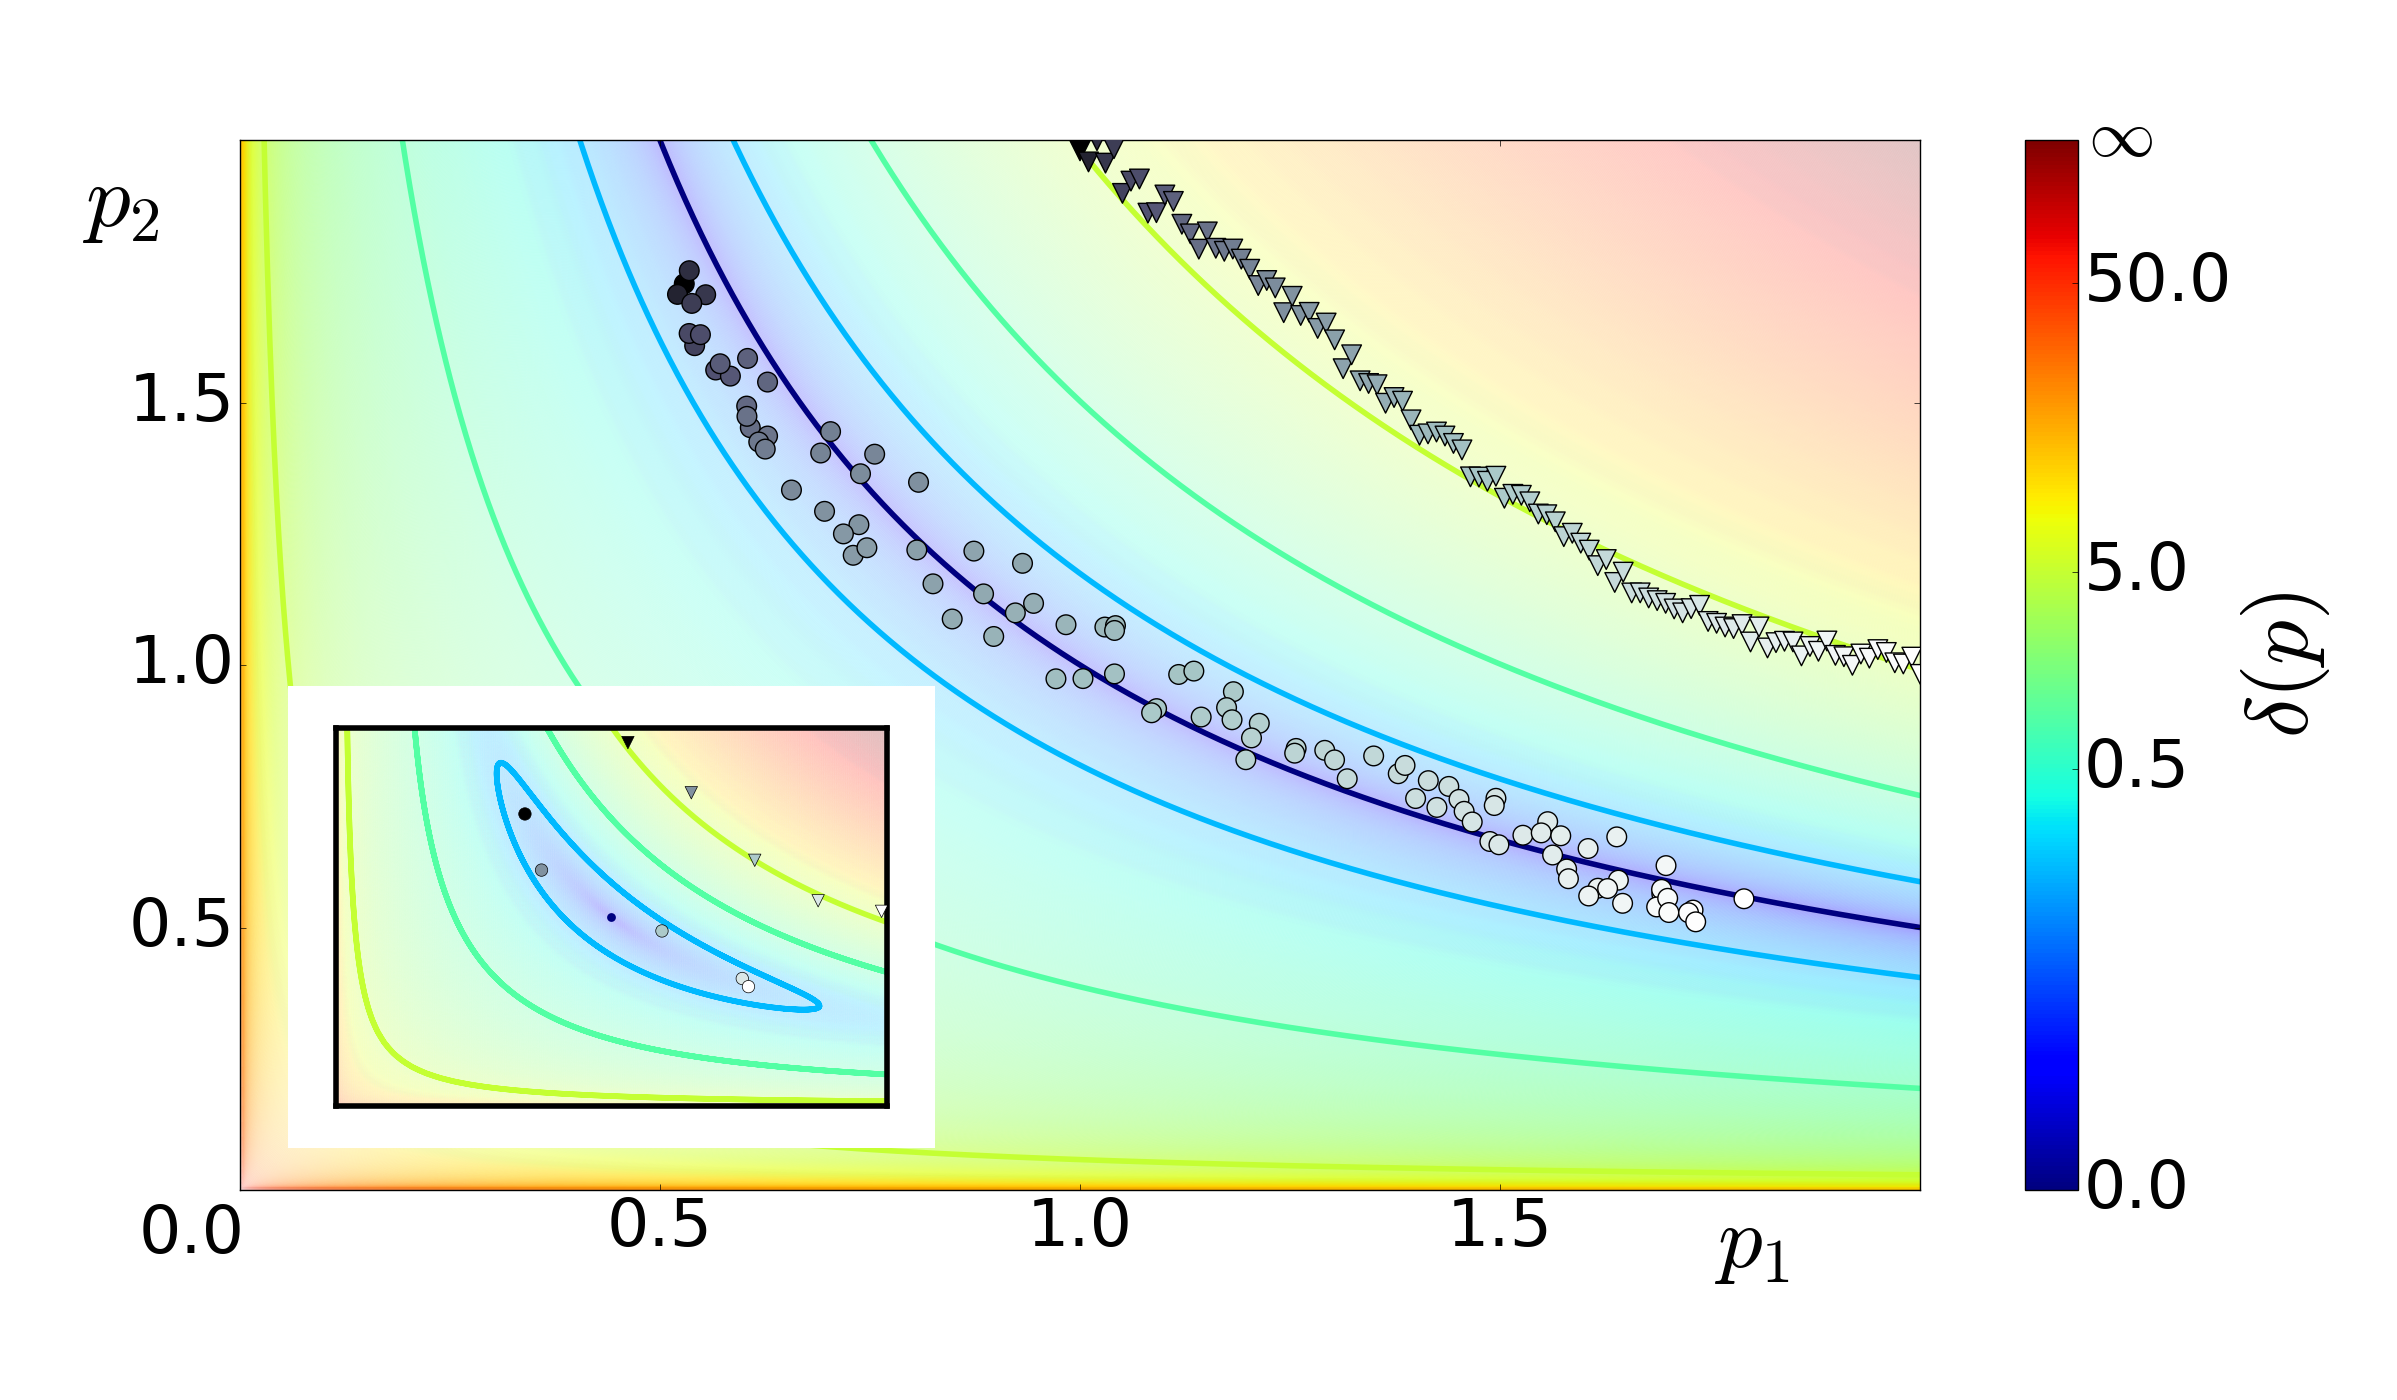
\includegraphics[width=1.0\linewidth]{p2-p1-delta}}
  \caption[Illustration of effects of sloppiness on
  optimization]{Coloring the $(p_1, p_2)$ plane by $\delta$ for
    $f(\theta) = (p_1 p_2 , \ln(p_1) + \ln(p_2) , (p_1 p_2)^2)$ (main
    figure) and the perturbed $g(p1, p2) = f(p_1, p_2) +
    \left(2*\epsilon*(p1 - p2), 0, 0\right)$ with $\epsilon = 0.2$
    (inset). $\delta$ values are calculated with respect to the base
    parameters $p^* = (1, 1)$: $\delta(p_1, p_2) = \| f(p_1, p_2) -
    f(p_1^*, p_2^*)\|$. Also shown are a range of initial and final values of
    a gradient descent algorithm. For $f$, convergence can occur
    anywhere along the infinite band for which $\delta$ is less than
    the accepted tolerance. For $g$, convergence is confined to
    bounded but stretched regions in the plane.
    \label{fig:non-id} }
\end{figure}



\section{Example from chemical kinetics} \label{sec:rr}

We now examine a system of chemical reactions in which an effective
parameter again emerges, and show how we can detect this in a
data-driven manner. The three-species system is

\begin{align}
  A
  \xrightleftharpoons[k_{-1}]{k_1}
  B
  \xrightarrow[]{k_2}
  C
  \label{mech:abc}
\end{align}

Under mass action kinetics, the concentration of the end product is
given by the analytical expression
% 
\begin{align}
  C(t|\theta)
  =
  A_0
  \left(
  \frac{k_1 k_2}{\alpha \beta}
  +
  \frac{k_1 k_2}{\alpha(\alpha - \beta)}
  e^{-\alpha t}
  -
  \frac{k_1 k_2}{\beta(\alpha - \beta)}
  e^{-\beta t}
  \right)
  \label{eq:cfull}
\end{align}
% 
where $(A_0,B_0,C_0)$ are the fixed constituent concentrations at time
zero and $\alpha,\beta$ depend on $\theta=(k_{-1},k_1,k_2)$; see
Appendix~\ref{app:abc} for the derivation. In the parameter regime
$k_1 k_2 \ll (k_1 + k_{-1} + k_2)^2$, \eqref{eq:cfull} is well
approximated by
% 
\begin{align}
  C_{eff}(t|\theta)
  =
  A_0
  \left(
  1 - e^{-k_{eff} t}
  \right) ,
  \quad
  k_{eff}
  =
  \frac{k_1 k_2}{k_{-1} + k_1 + k_2} .
  \label{eq:abc-qssa}
\end{align}
% 
Note that this approximate solution extends to a larger parameter
range the quasi-steady state approximation (QSSA)
$C_\mathrm{QSSA}(t|\theta) = A_0 (1 - e^{-k_\mathrm{QSSA} t})$, valid
for $k_1 \ll k_{-1} + k_2$ with
$k_\mathrm{QSSA}=k_1 k_2/(k_{-1} + k_2)$.  Plainly, this approximate
solution represents an effective reduction of parameter space down to
the single parameter $k_{eff}$, the levels sets of which foliate
parameter space as in Fig.~\ref{fig:abc-ill}.

To verify that $C(t)$ remains roughly constant on these level sets, we
choose reference parameter settings $\theta^*$ in the regime
identified above, fix sampling times $t_1,\ldots,t_N$, set the model
response to $f(\theta)=( C(t_1|\theta) , \ldots , C(t_N|\theta) )$,
sample log-parameter space uniformly, and record the squared Euclidean
distance $\delta(\theta) = \| f(\theta) - f(\theta^*) \|^2$ for each
sampled $\theta$.  Figure~\ref{fig:abc-keff} shows the results colored
by $k_{eff}$. We only retained parameter combinations with
$\delta(\theta) < 10^{-6}$ to aid in visualization. As expected, the
level sets of constant $\delta$ align with those of the effective
parameter, so this automated sampling process effectively reveals
sheets of different $k_{eff}$ values without recourse to an analytic
expression.

\begin{figure}[!htp]
  \centering
  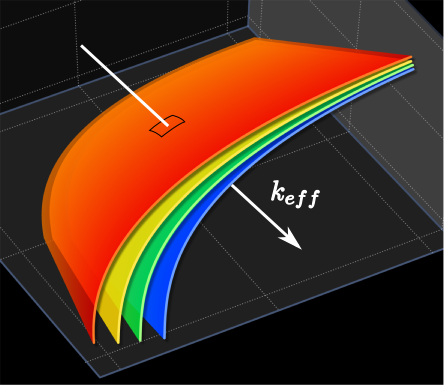
\includegraphics[width=0.4\textwidth]{keff-illustration}
  \caption[Illustration of level sets of the effective parameter in a
  model of chemical kinetics]{Illustration of level sets of $k_{eff}$
    in parameter space. \label{fig:abc-ill}}
\end{figure}


\begin{figure}[ht!]
  \centering
  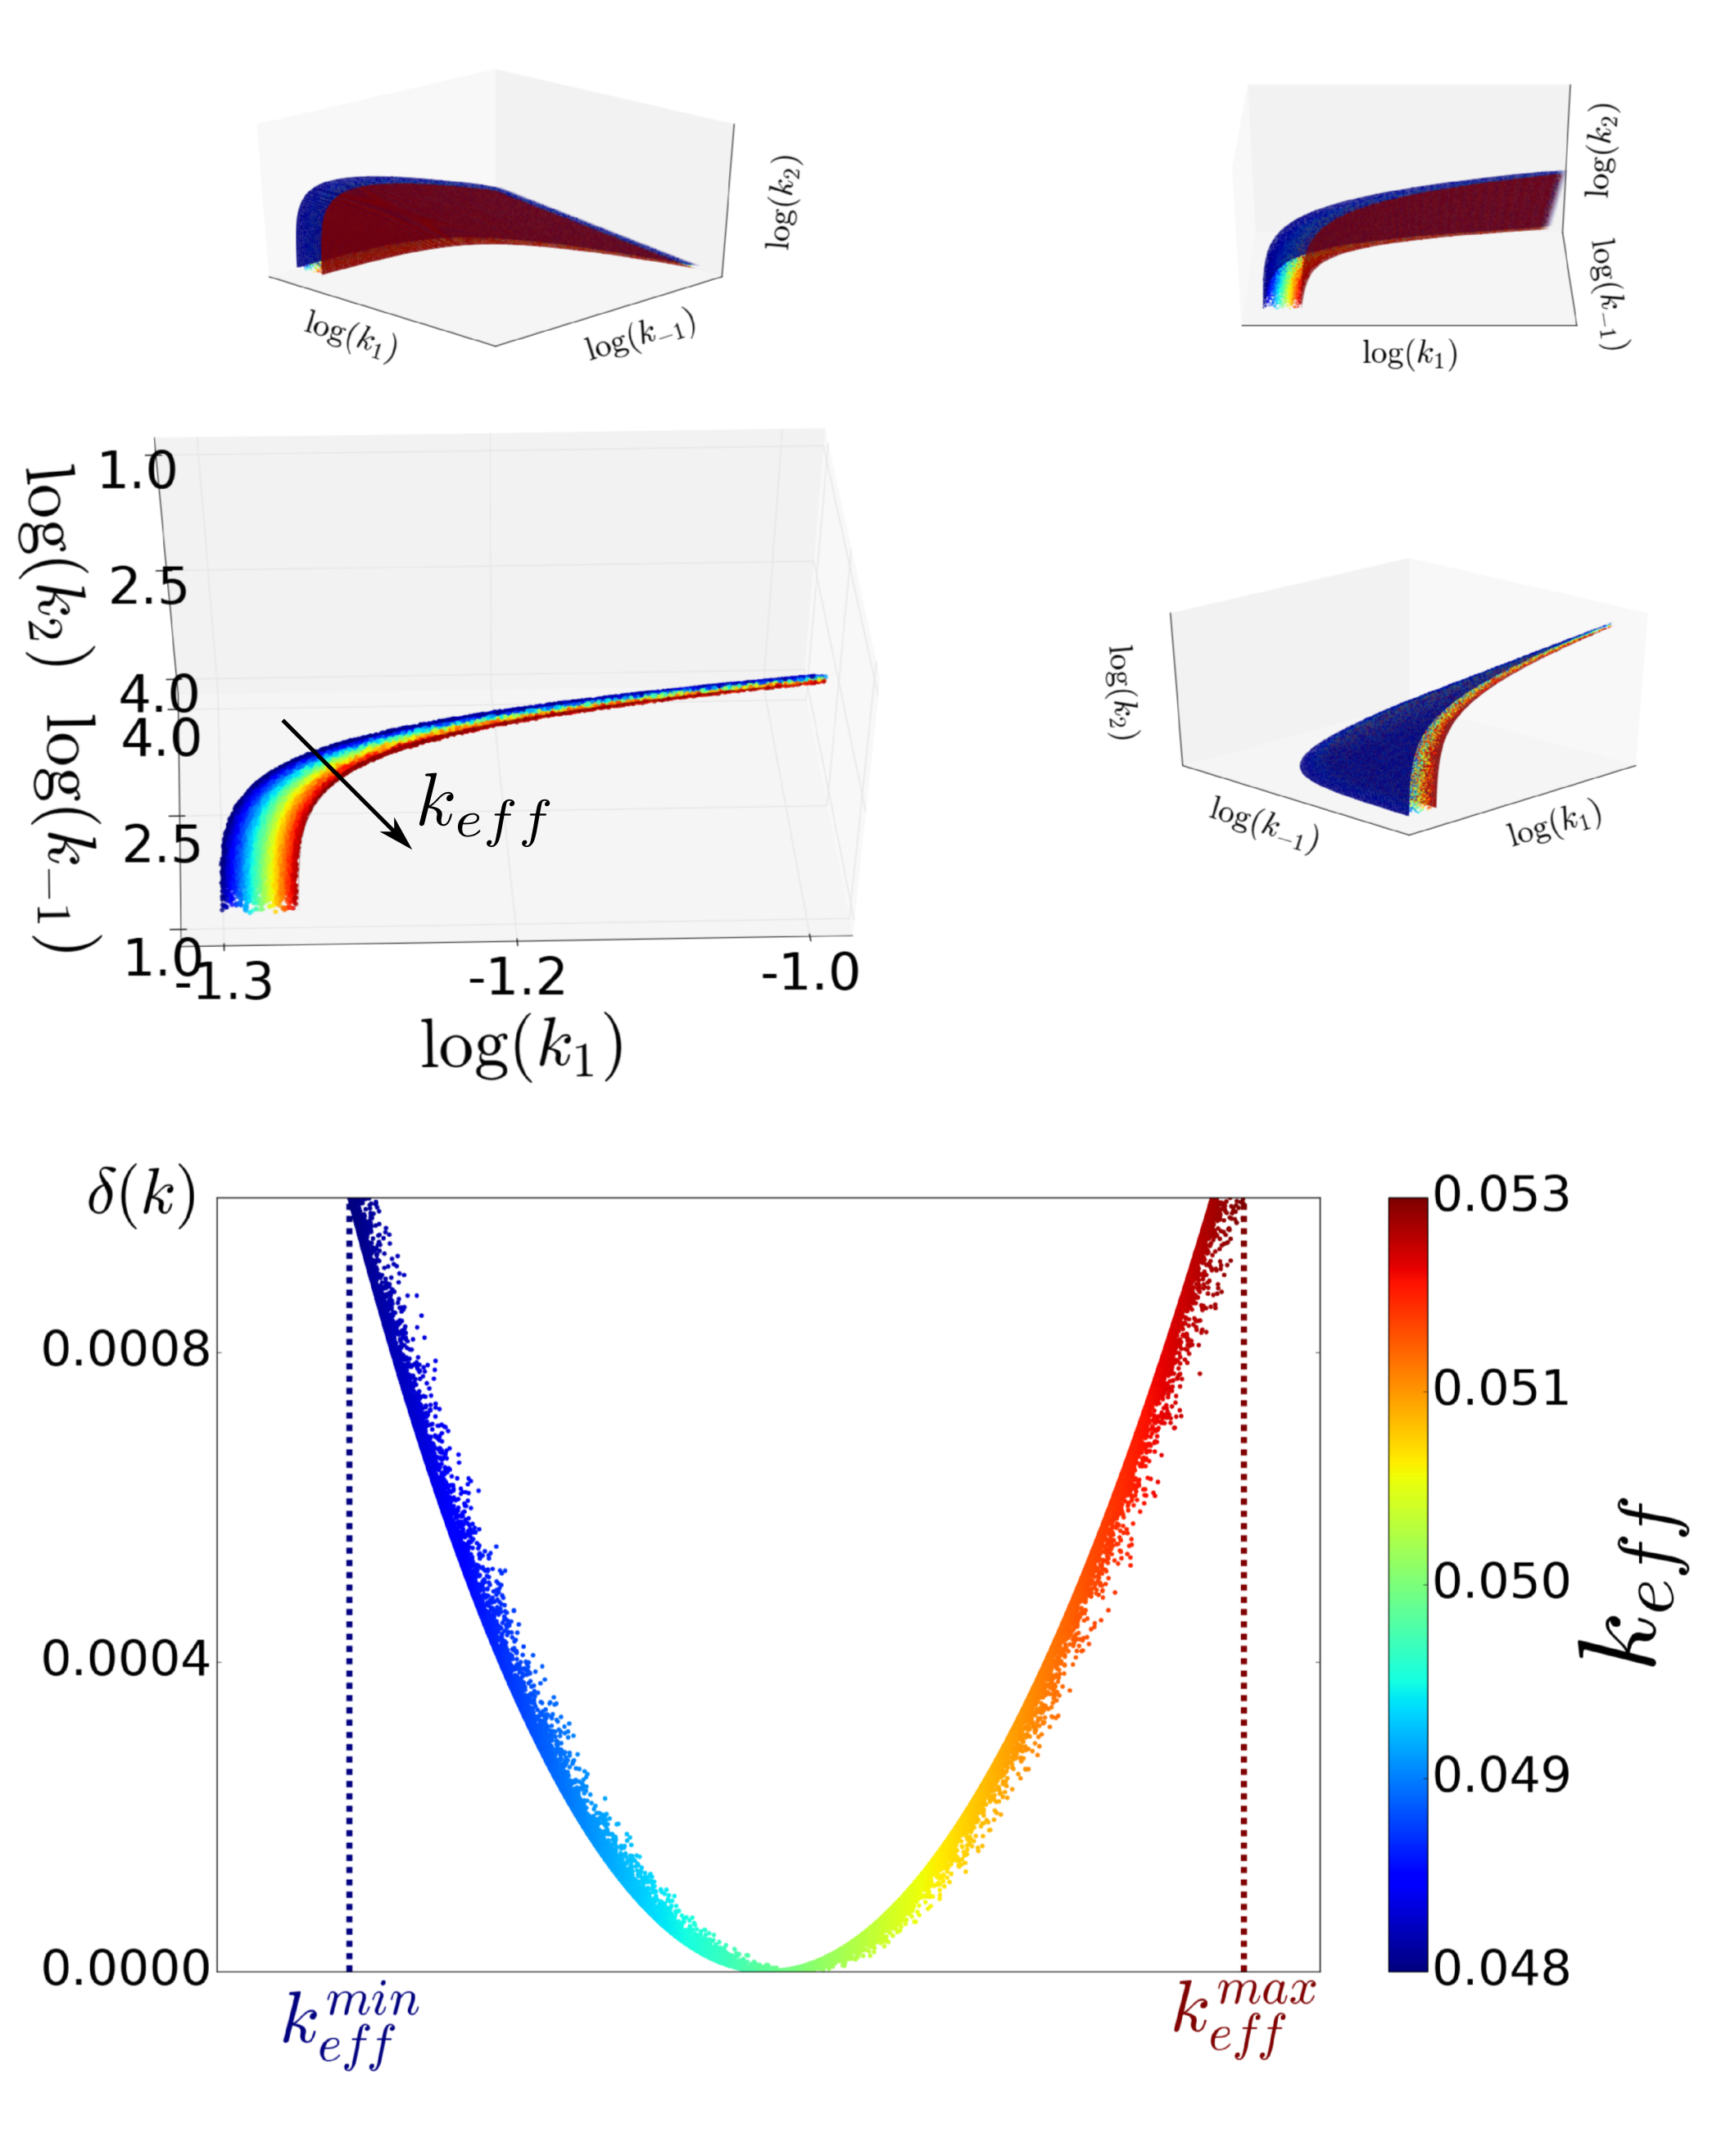
\includegraphics[width=0.9\textwidth]{keffs-delta-keff-vertical}
  \caption[Quantitative three-dimensional views of level sets of the
  effective parameter in a model of chemical kinetics]{(top) Region of
    parameter space lying within large value of $\delta = 10^{-3}$,
    colored by $k_{eff}$. Smaller rotations show three-dimensional
    structure. (bottom) Plot of $\delta$ vs $k_{eff}$ over the dataset
    showing that $\delta(k_1, k_{-1}, k_2) = \delta(k_{eff})$ as
    expected from the reduced reaction kinetics. \label{fig:abc-keff}}
\end{figure}


\begin{figure}[!htp]
  \centering
  \begin{tabular}{cc}
    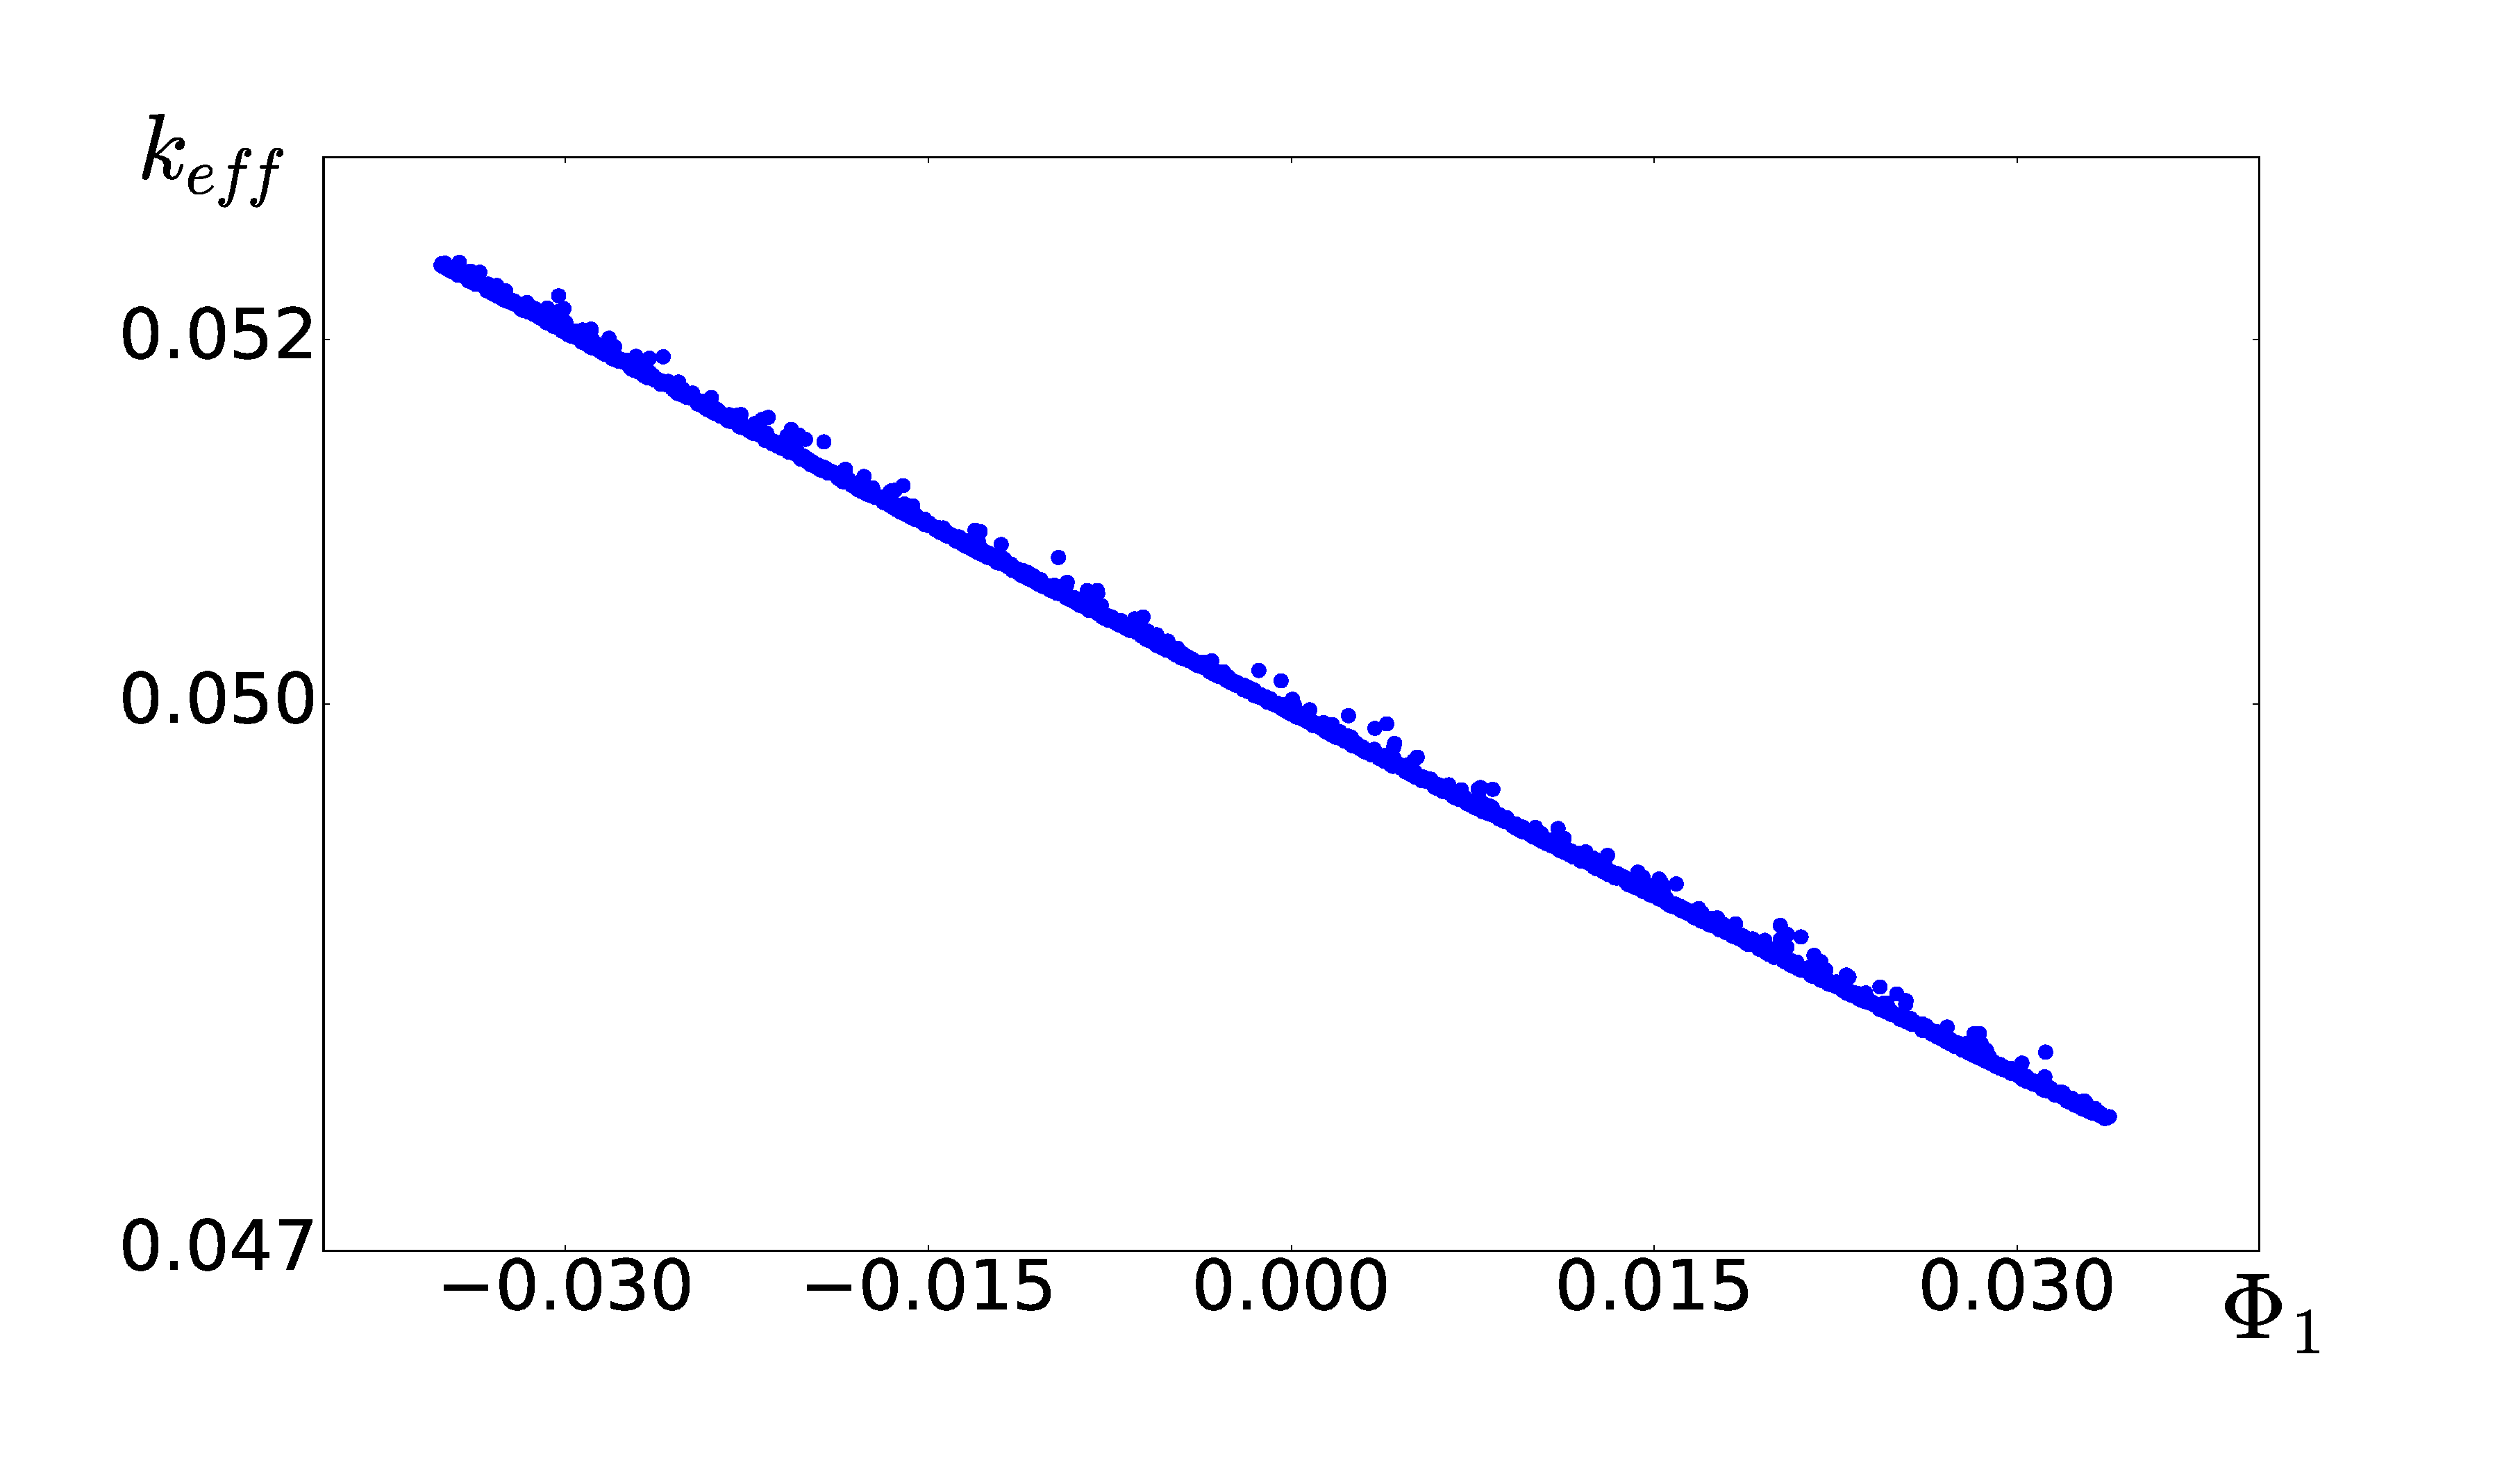
\includegraphics[width=0.45\textwidth]{keff-phi1} &
                                                        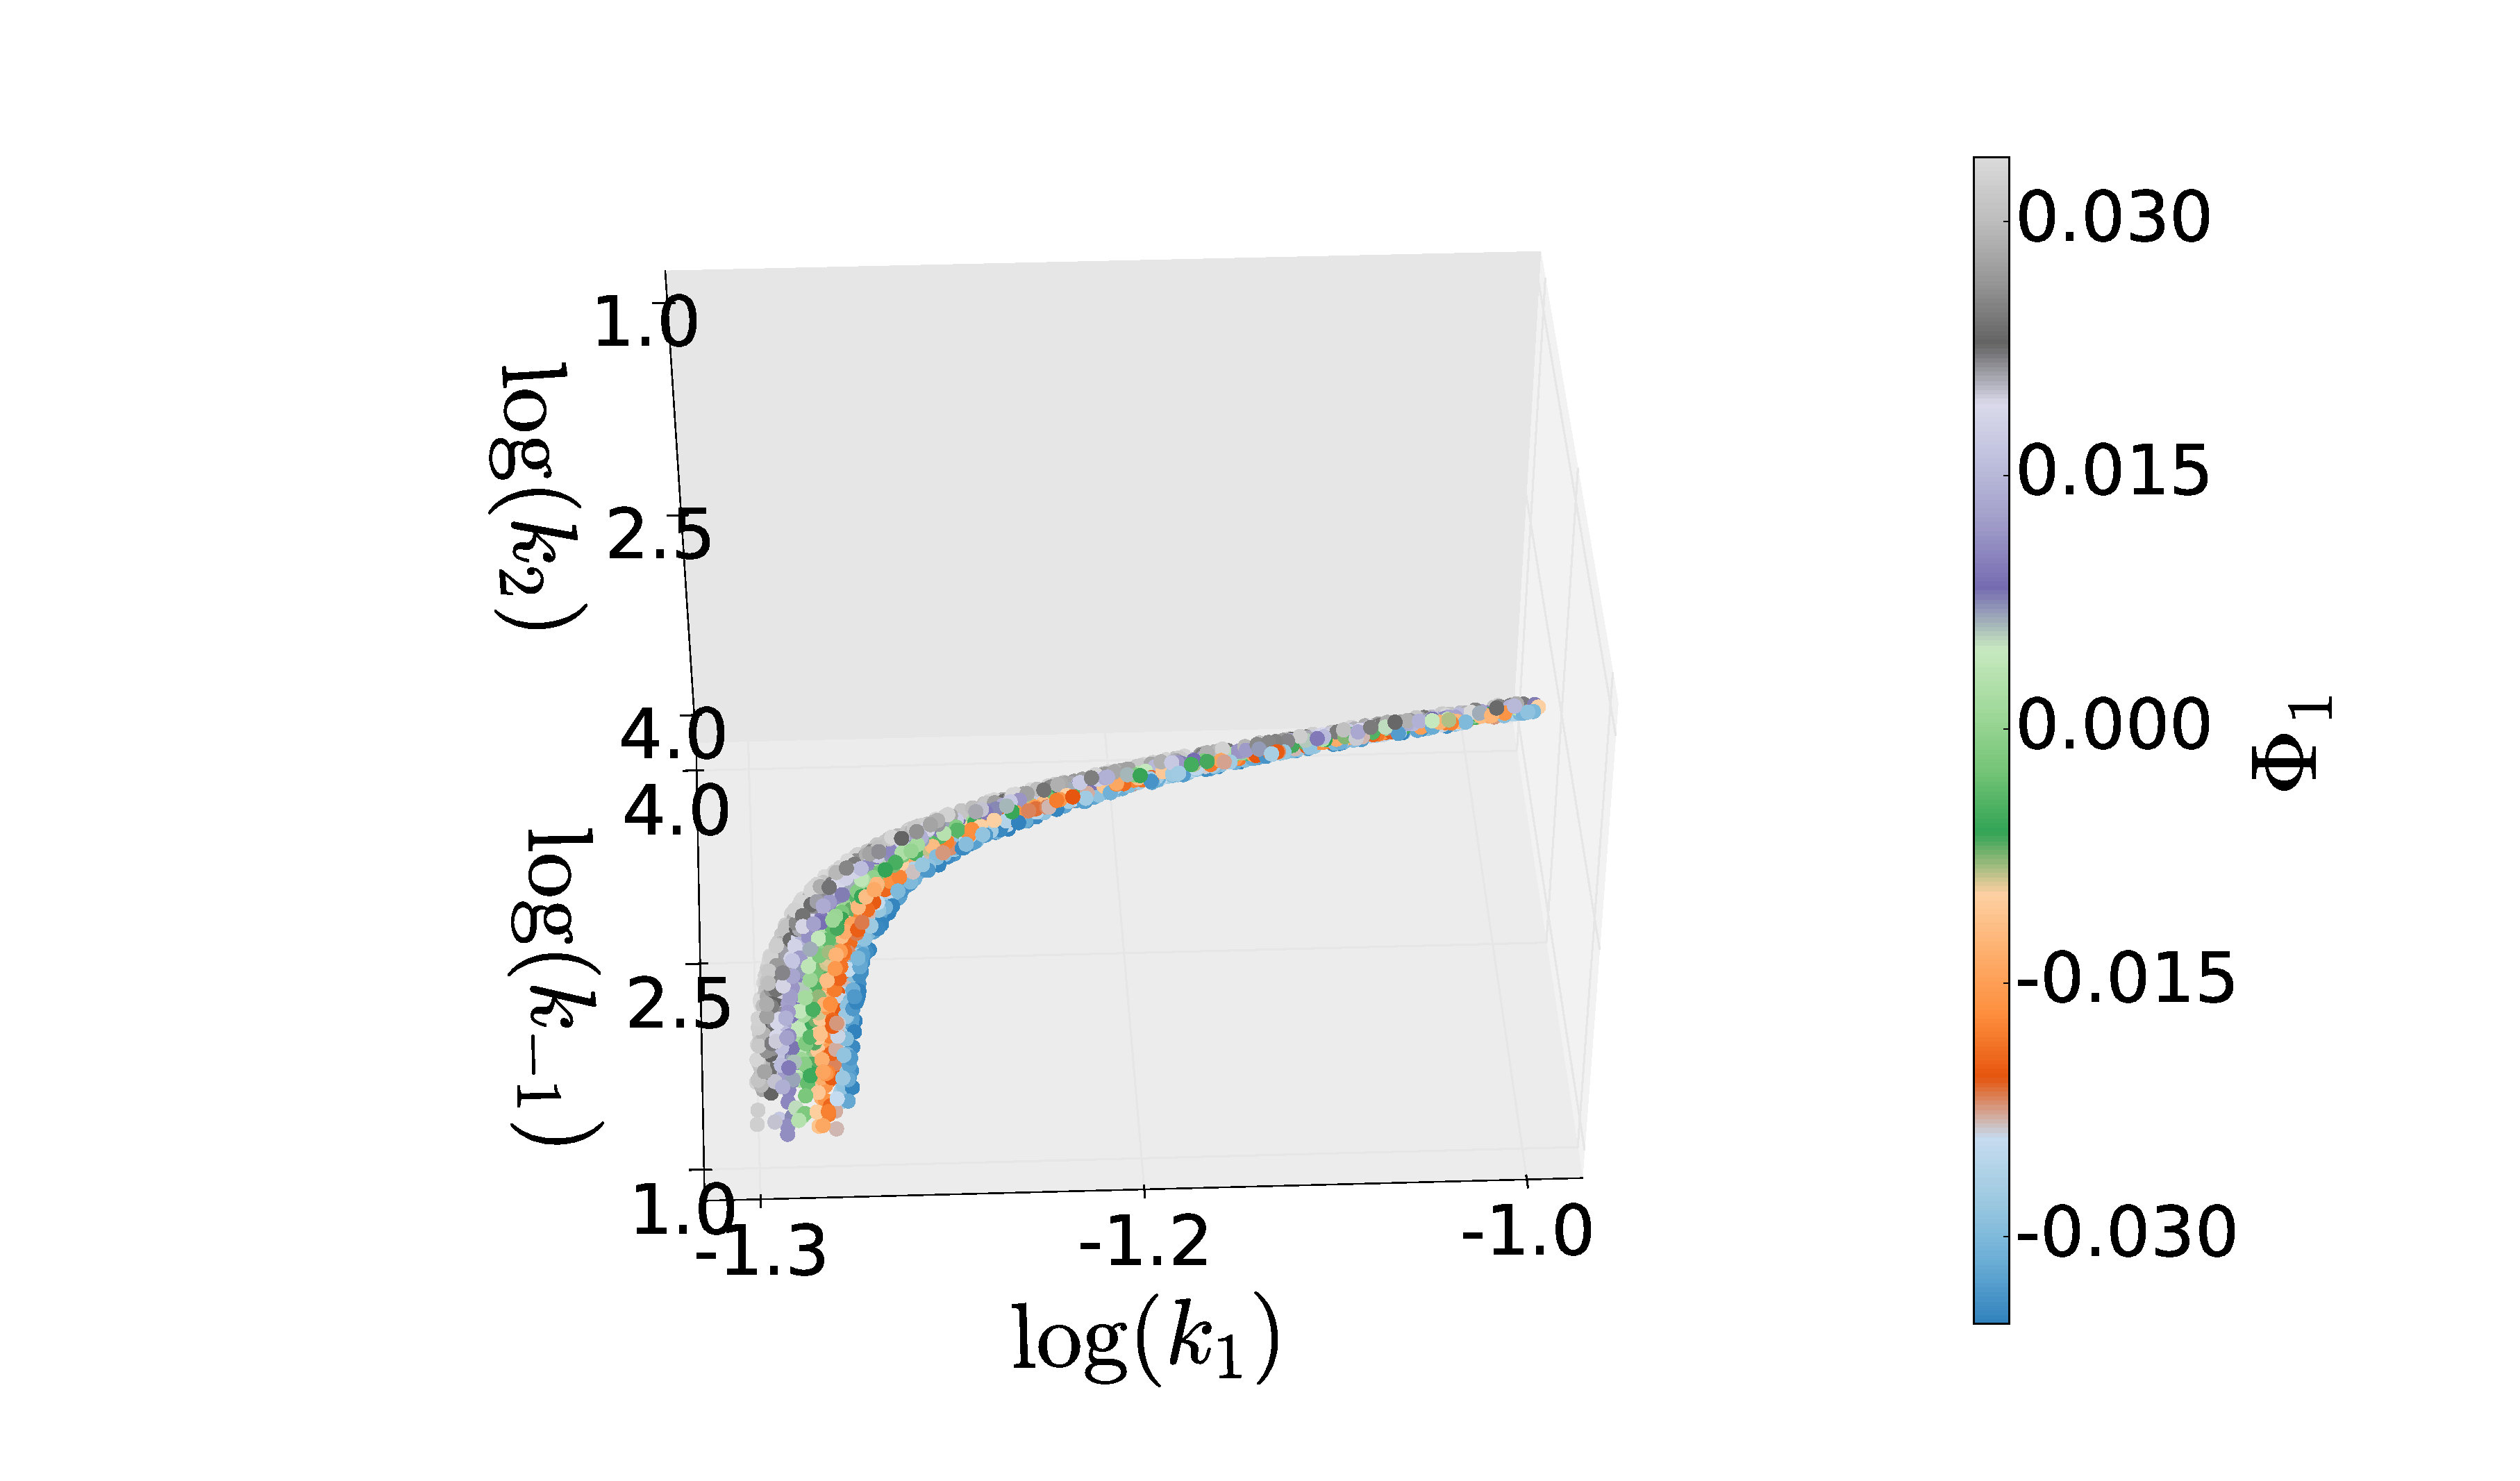
\includegraphics[width=0.5\textwidth]{k2-kinv-k1-phi1}\\
    (a) & (b)
  \end{tabular}
  \caption[DMAPS results for simple kinetic model]{(a) Coloring parameter space by $\phi_1$, showing that
    $\phi_1$ captures the effective parameter in this system; (b)
    $k_{eff}$ plotted against $\phi_1$ showing that the first DMAPS
    eigenvector parameterizes the significant, nonlinear parameter
    combination hidden in our model. \label{fig:abc-dmaps}}
\end{figure}


With this data in hand, we turn to a description of our modified
DMAPS algorithm. Details of the basic algorithm can be found in
Section~\ref{sec:dmaps}. In brief, given a collection of parameter
values ${\theta_i}_{i=1}^N$, we define our DMAPS kernel as

\begin{align}
  k(\theta_i, \theta_j) = \exp \left(-\frac{\|f(\theta_i) -
  f(\theta_j)\|^2}{\epsilon^2} \right)
  \label{eq:dmaps-mm}
\end{align}

The key point is that while the data in Figure~\ref{fig:abc-keff}
obviously represent a sample of parameter space, they simultaneously
sample the model response space through $f(\theta)$. Considering the
structure of this space, we can understand that all of the points
lying on a surface of constant $k_{eff}$ will be mapped to
approximately the same point in model response space: they share the
same output concentration trajectory as seen in
Equation~\ref{eq:abc-qssa}. Only changes in $k_{eff}$ affect the model
output, and thus our data will lie along a one-dimensional curve in
model response space, parameterized by $k_{eff}$. Therefore, if we
apply DMAPS to the model response data, the first eigenvector $\phi_1$
will yield a parameterization of this curve and we expect $k_{eff}$
and $\phi_1$ to be in one-to-one correspondence. This is precisely
what Figures~\ref{fig:abc-dmaps} shows. DMAPS has, in effect,
uncovered the effective parameter hidden in the system using only
parameter and model response data. We will now investigate how
sloppiness can arise in singularly- and regularly-perturbed systems,
and we will see that DMAPS is able to provide a more uniformly
significant reparameterization.


\section{Regular perturbation}

Let us now consider the differential equation
%
\begin{equation}
  \frac{dy}{dt} = \epsilon y^3 - y
  \quad
  y(0) = y_0 ,
  \label{1D-model-regpert}
\end{equation}
%
with $\theta = (y_0, \epsilon)$ and
$f(\theta) = \left(y(t_1), y(t_2), \dots, y(t_n) \right)$.

Unlike the previous two examples, there is no effective parameter
hidden in this system; however, our parameters affect the model output
very differently depending on their specific values. To see why this
is, consider what happens as $\eps \rightarrow 0$. The system becomes
regularly perturbed, and converges to the simpler
$\frac{dy}{dt} = -y$. Note that in this limit, $\eps$ has no influence
on the model response, and $y_0$ becomes the only significant
parameter. Again, considering the implications for the model manifold,
it is clear that for small values of $\eps$, our response will form a
one dimensional curve parameterized by $y_0$. At larger values, both
$\eps$ and $y_0$ are significant, and the manifold is
two-dimensional. Figure~\ref{fig:regpert} (a) depicts the model
manifold colored by $\eps$, and we see exactly this behavior. The red
portion of the surface, corresponding to larger $\eps$, is
two-dimensional, while the blue, with small $\eps$, is contained in a
single line at the edge of the surface. Sampling this manifold, as
detailed in Appendix~\ref{app:regpert}, and applying DMAPS with the
kernel presented in Equation~\ref{eq:dmaps-mm} yields the same
information directly from data. Figure~\ref{fig:regpert} (b) shows the
$(\eps, y_0)$ parameter plane colored by $\phi_1$. At larger values of
$\eps$ the colors vary without any significant trend as this region is
two-dimensional. However, at small $\eps$, the colors flatten out
horizontally: $\phi_1$ is constant along lines of constant
$y_0$. DMAPS captures the fact that only one direction in parameter
space is relevant in the regularly perturbed regime. To continue along
this line in a slightly more complicated scenario, our next system
will be singularly perturbed.

\begin{figure}[ht!]
  \centering
  \begin{tabular}{cc}
    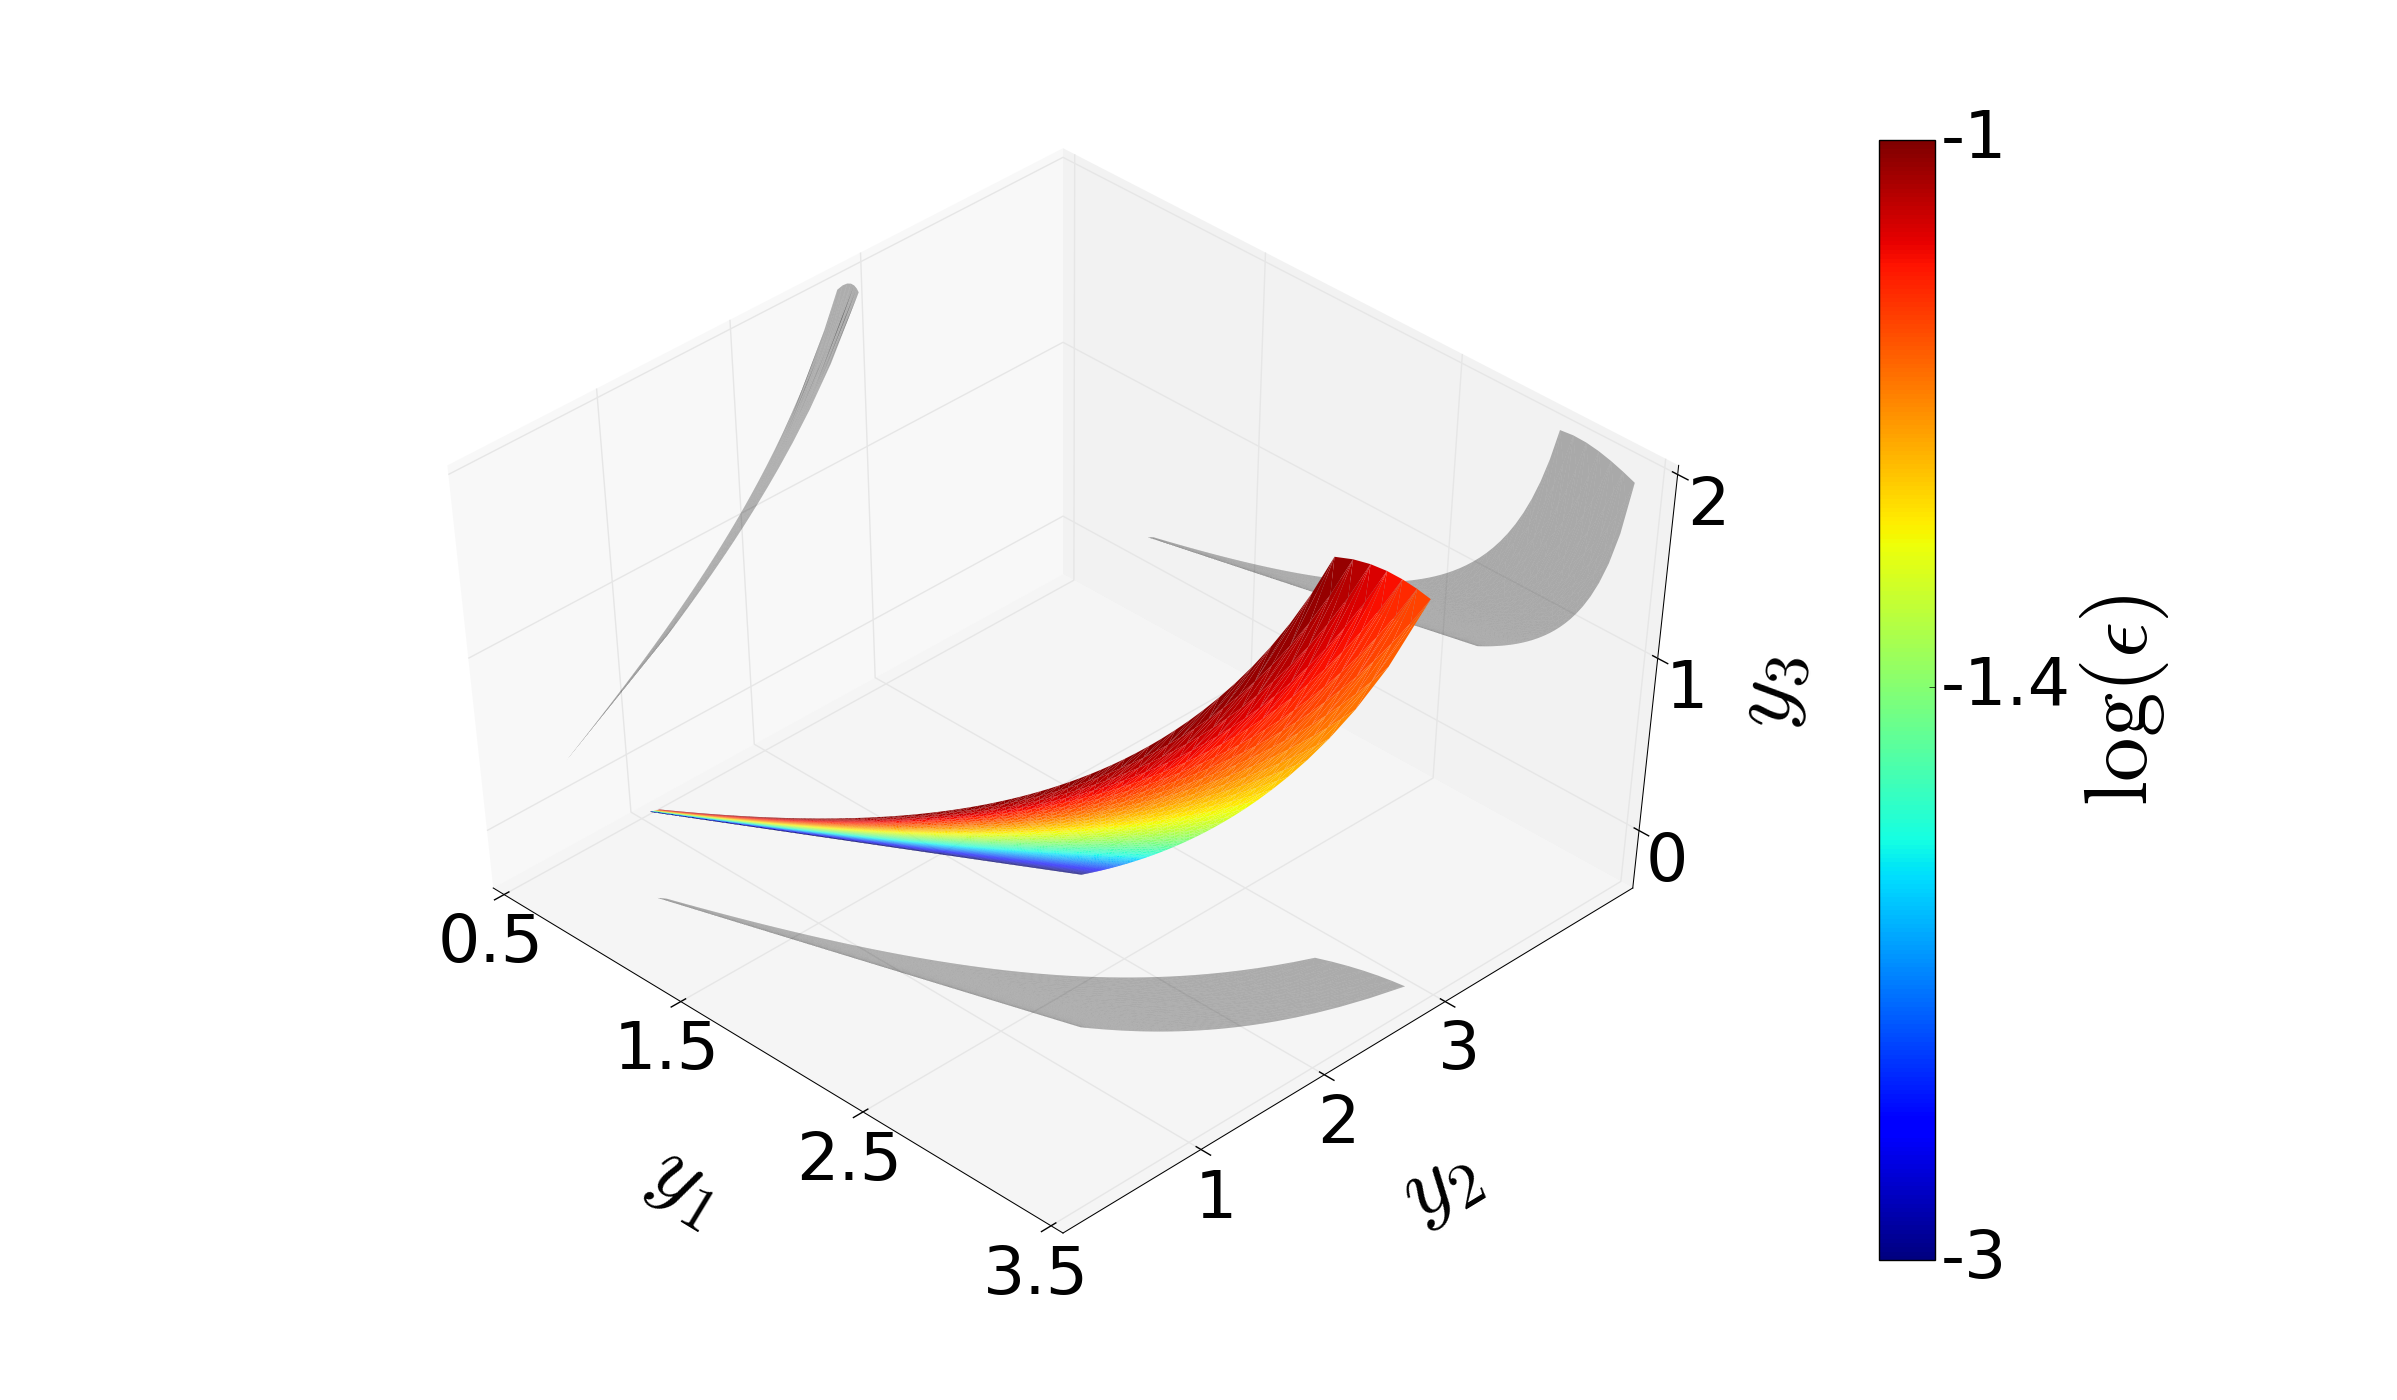
\includegraphics[width=0.5\textwidth]{y3-y2-y1-eps} &
                                                           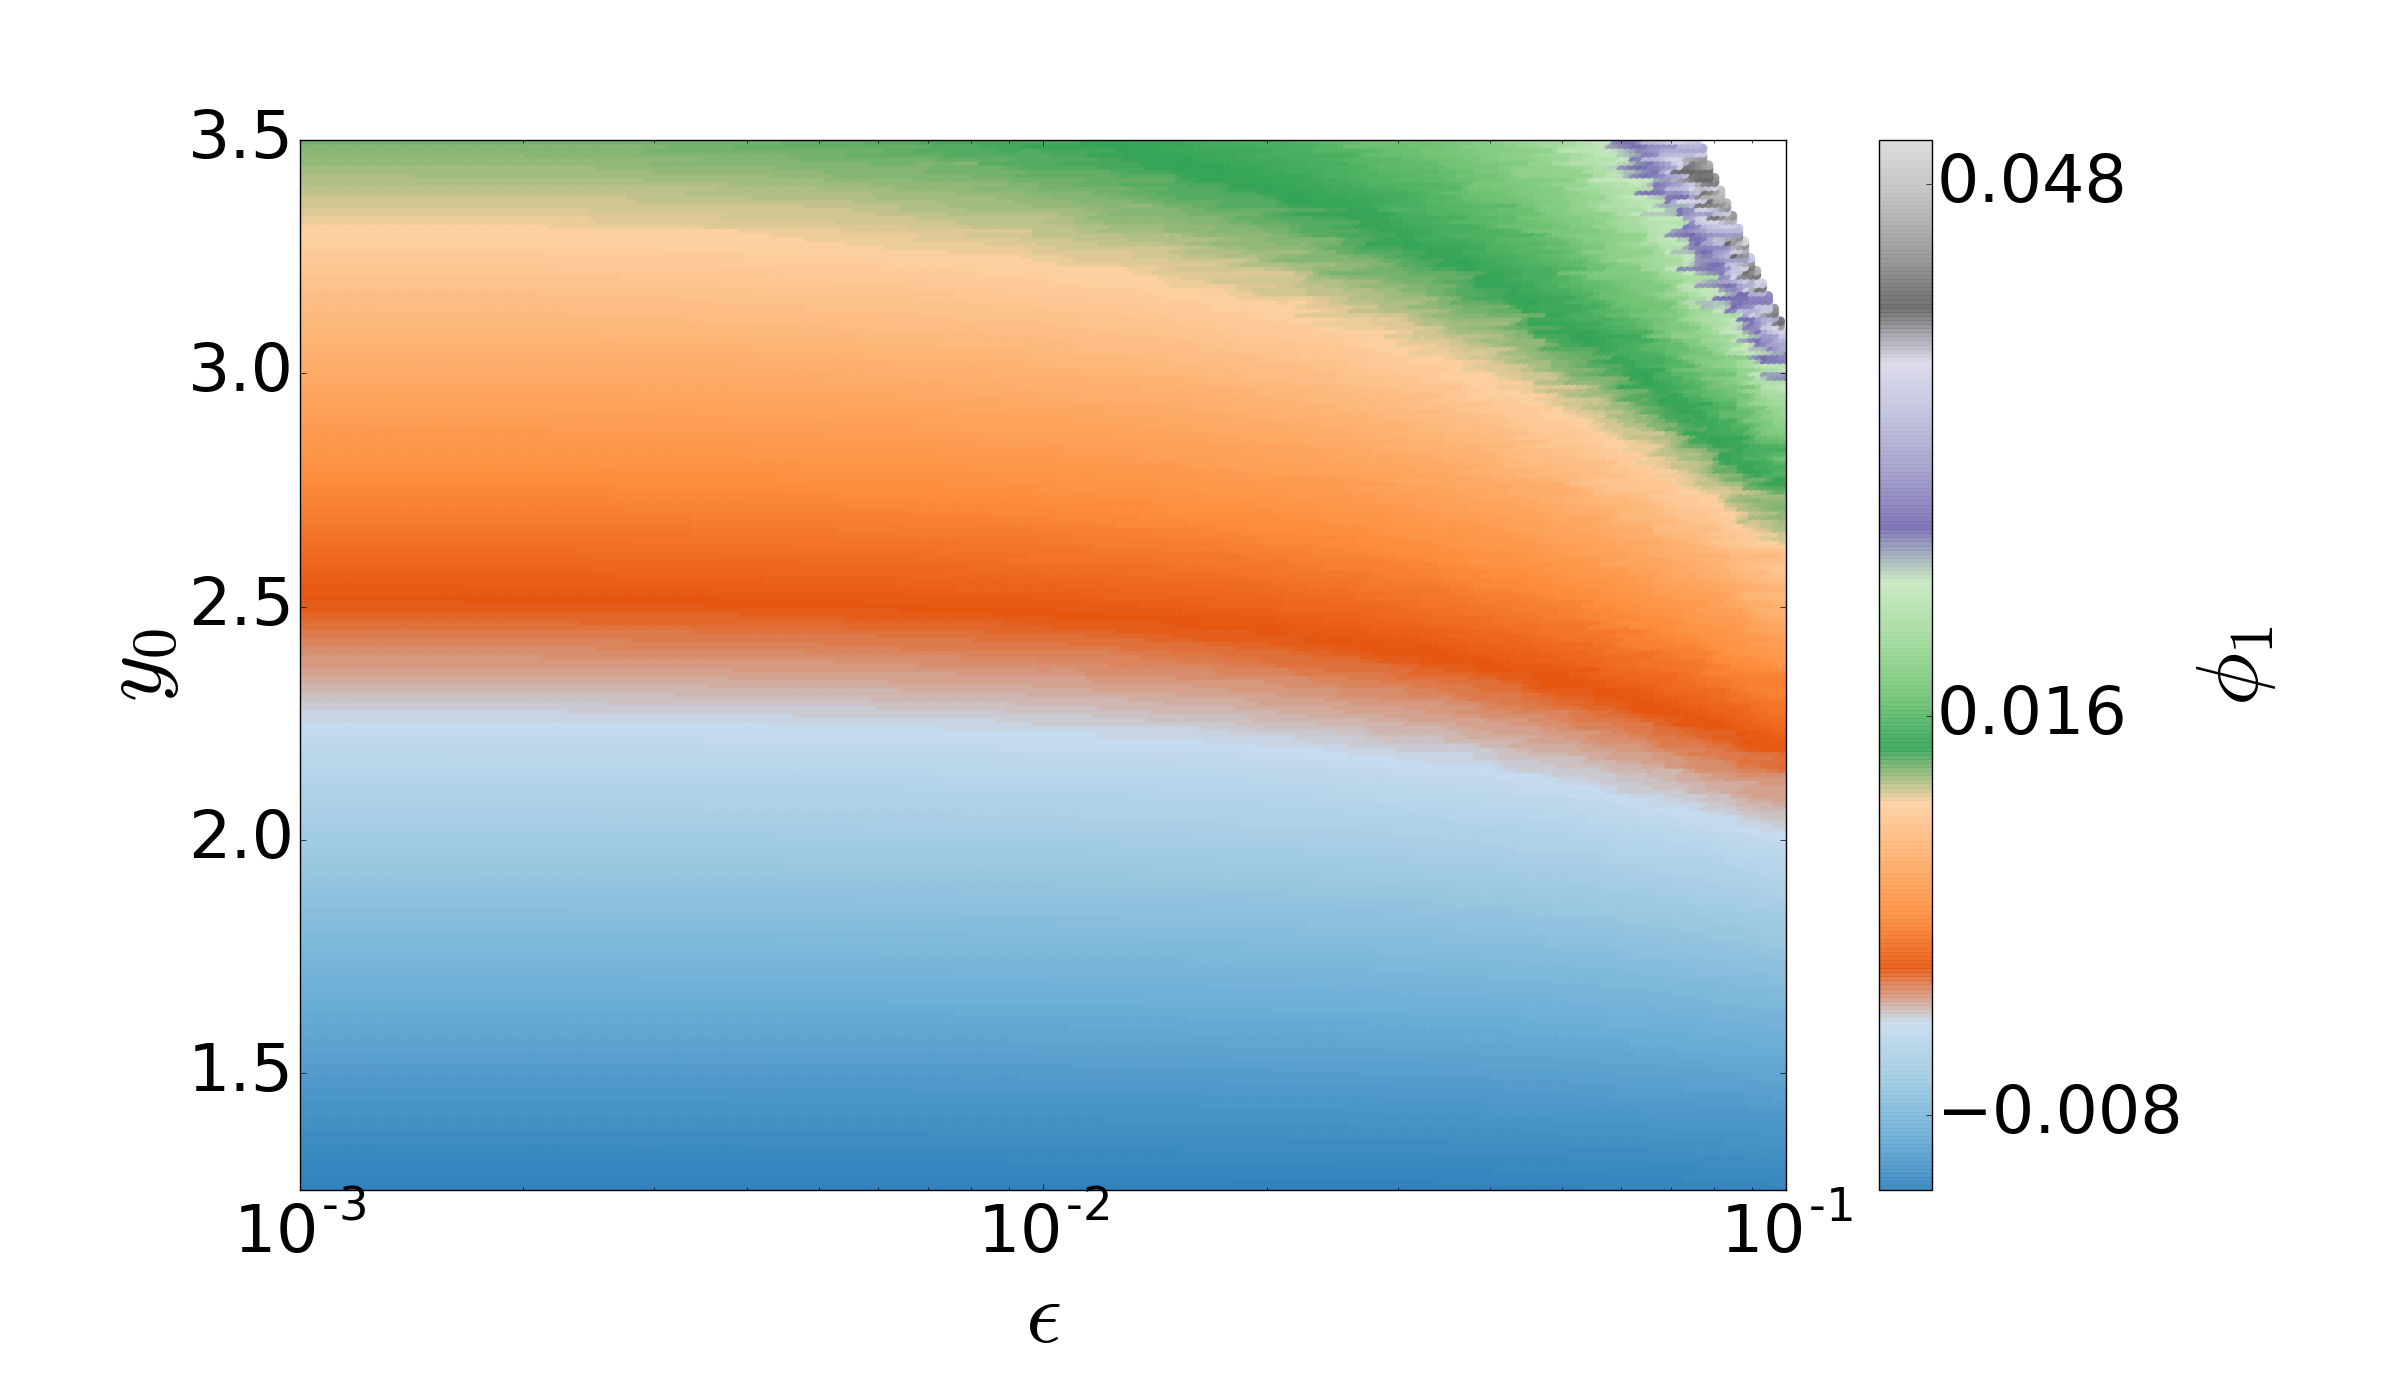
\includegraphics[width=0.5\textwidth]{y0-eps-phi1} \\
    (a) & (b)\\
  \end{tabular}
  \caption[Model manifold and parameter space of regularly perturbed system]{(a) Model manifold of regularly perturbed system with
    parameters $y_0$ and $\epsilon$, colored by $\epsilon$. As
    $\epsilon$ decreases, the model response is increasingly
    determined solely by $y_0$ as the system converges to $y' = -y$;
    (b) Parameter space colored by $\phi_1$ for the regularly
    perturbed system. As $\epsilon$ decreases, only the value of $y_0$
    is significant. This is captured by DMAPS as $\phi_1$ varies only
    vertically, in the $y_0$ direction, at small
    $\epsilon$. \label{fig:regpert}}
\end{figure}


\section{Singular perturbation}

The system is now given by

\begin{align}
  \frac{dx}{dt}&=2-x-y\\
  \frac{dy}{dt}&= \frac{1}{\epsilon}(x-y)
\end{align}    

with $\theta = (y_0, \epsilon)$ and
$f(\theta) = \left(y(t_1), y(t_2), \dots, y(t_n) \right)$ as
before. At small values of $\eps$ the equations become singularly
perturbed, and we cannot simply set $\eps = 0$ to find our reduced
description as before. Instead we see that $y$ will rapidly approach
the slow manifold $y = x$, and then progress towards the steady state
$(x,y) = (1,1)$. The phase portrait for this system is shown in
Figure~\ref{fig:singpert}.

Crucially, on the slow manifold our system is approximately
one-dimensional, governed by $\frac{dx}{dt} = -2 - 2x$. If we choose
our sampling times $t_1, t_2, \dots, t_n$ based on the slow timescale
of the system, our dynamics will be one-dimensional, and in fact
neither $\eps$ nor $y_0$ will affect the model response. At small
$\eps$, $y$ quickly converges to the slow manifold (order $\eps$
time), and then slowly evolves toward the stationary state. At
$\eps \ll 1$, our model manifold converges to a single,
zero-dimensional point. Whereas in the regularly perturbed example we
transitioned from two to one significant parameters, singular
perturbation brings a transition from two to zero. If we have obtained
a sample of the $(\eps, y_0)$ parameter plane, we can again apply
DMAPS to re-parameterize the system. Figure~\ref{fig:singpert-dmaps}
shows the results of such an analysis. In
Figures~\ref{fig:singpert-dmaps} (a) and (d) we have colored the
parameter plane by $\phi_1$ and $\phi_2$, analogous to
Figure~\ref{fig:regpert} (b). Both eigenvectors are constant at small
$\eps$ reflecting the complete absence of significant parameters in
this regime. At larger $\eps$, $\phi_1$ and $\phi_2$ vary
independently as this corresponds to the two-dimensional region of the
manifold. Both $(\eps, y_0)$ and $(\phi_1, \phi_2)$ can be used to
parameterize the system, but whereas there are distinct regions in
which $\eps$ and $y_0$ become irrelevant, $\phi_1$ and $\phi_2$ are
consistently significant. DMAPS provides an automated and improved
parameterization of the system.

To clarify the relationship between parameter space, the model
manifold and the DMAPS embedding, we plot these three views of the
singularly perturbed system in Figure~\ref{fig:singpert-patches}. We
also color four different patches and track their transformation from
one space to the next. The yellow rectangle at larger $\eps$ is mapped
to a slightly deformed rectangle in both the model manifold and DMAPS
embedding. The blue patch, which approaches the singularly perturbed
regime, becomes stretched at the tip. The red patch is compressed to
an apparently one-dimensional line, while the green patch, lying
solidly within the singularly perturbed region, is mapped to a single
point in both alternative spaces. This represents the fact that in the
limit of small $\eps$, neither $y_0$ nor $\eps$ influence the model
output: everything collapses to a zero-dimensional point.

\vspace{1cm}
\begin{figure}[!htp]
  \centering
  \includegraphics[width=0.4\textwidth]{sample_traj_sing}
  \caption[Phase portrait for singularly perturbed system]{The phase portrait of the singularly perturbed system for
    different initial conditions; solid lines: $\epsilon=0.02$, dotted
    lines are $\epsilon=0.12$. \label{fig:singpert}}
\end{figure}

\begin{figure}[!htp]
  \centering
  \begin{tabular}{ccc}
    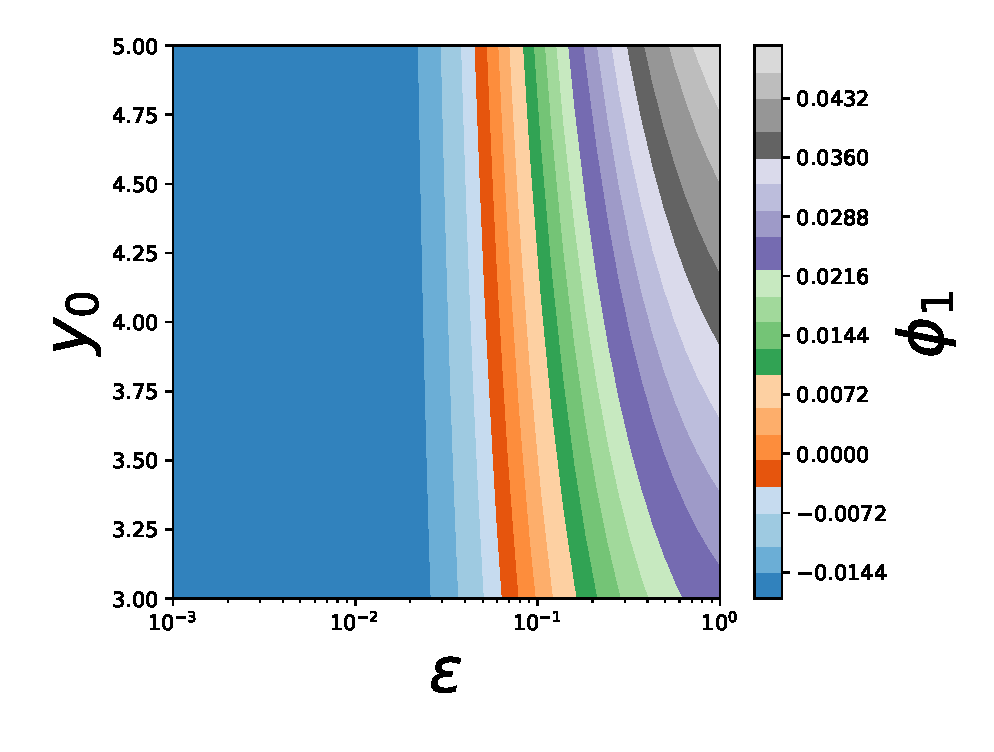
\includegraphics[width=0.33\textwidth]{y0_eps_phi1_sing} &
                                                               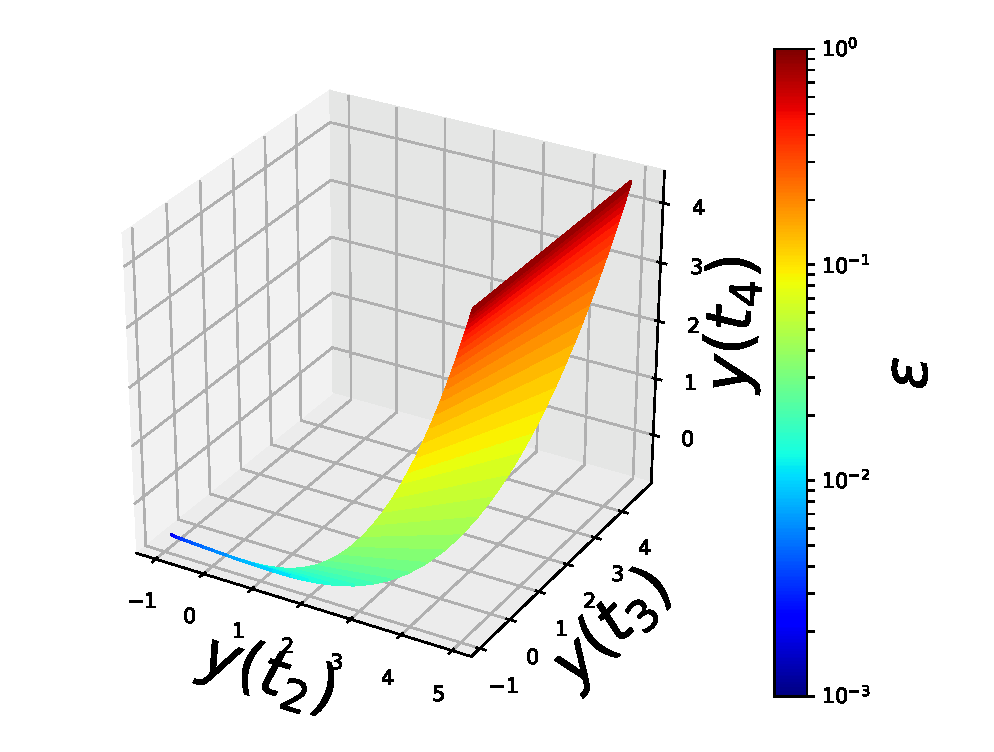
\includegraphics[width=0.33\textwidth]{mod_man_epsilon} &
                                                                                                                         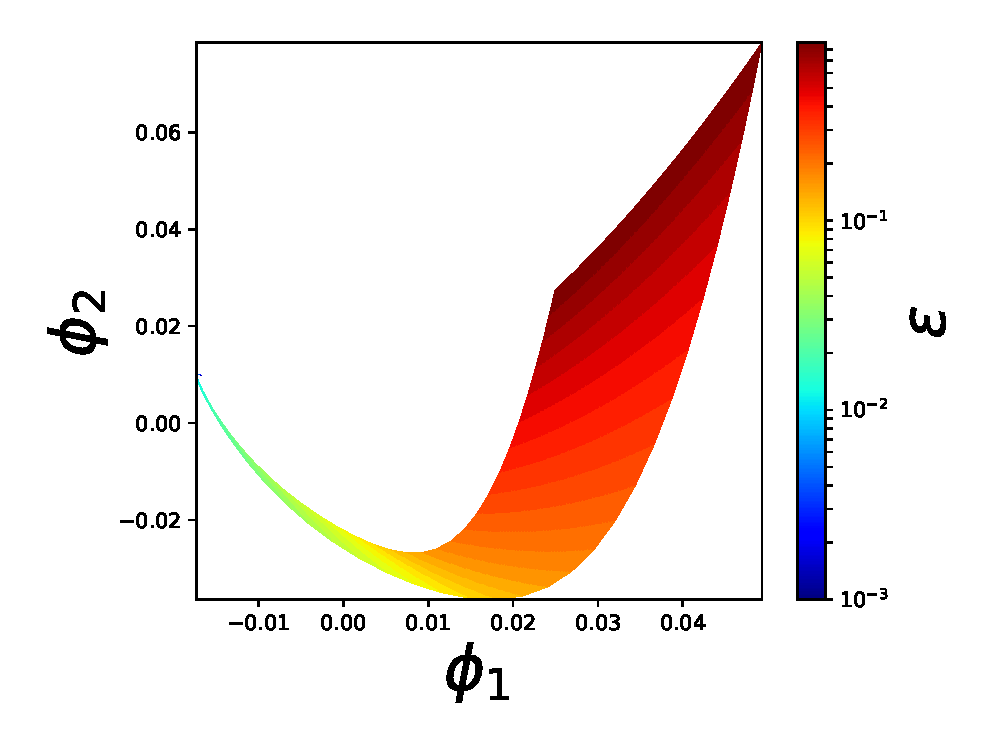
\includegraphics[width=0.33\textwidth]{phi2_phi1_eps_sing} \\
    (a) & (b) & (c)\\
    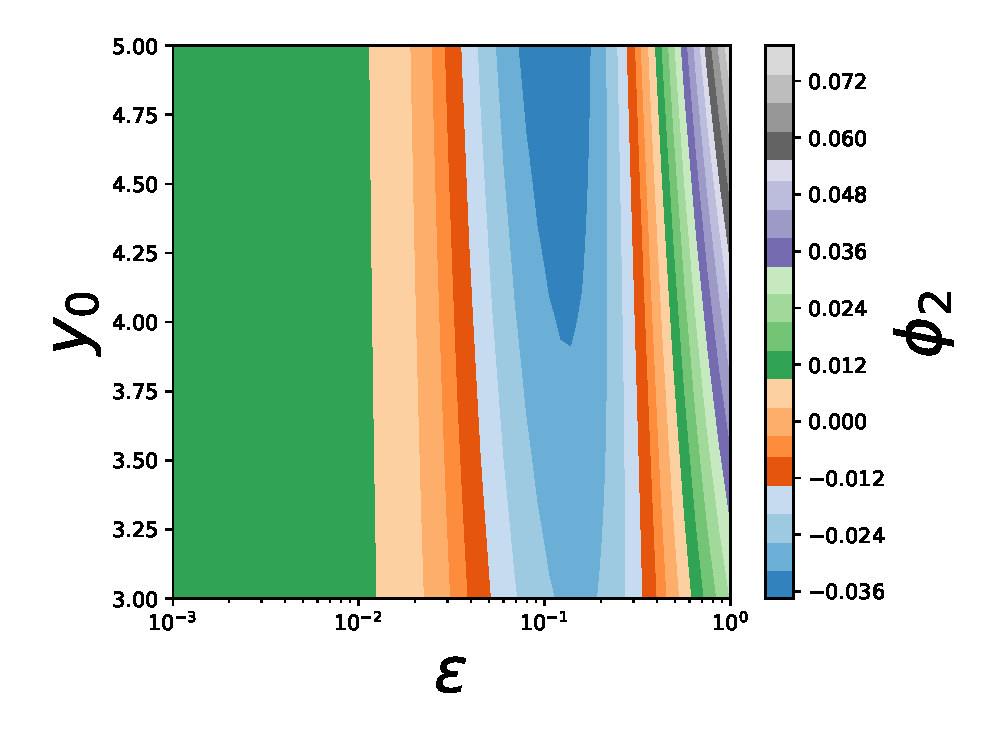
\includegraphics[width=0.33\textwidth]{y0_eps_phi2_sing} &
                                                               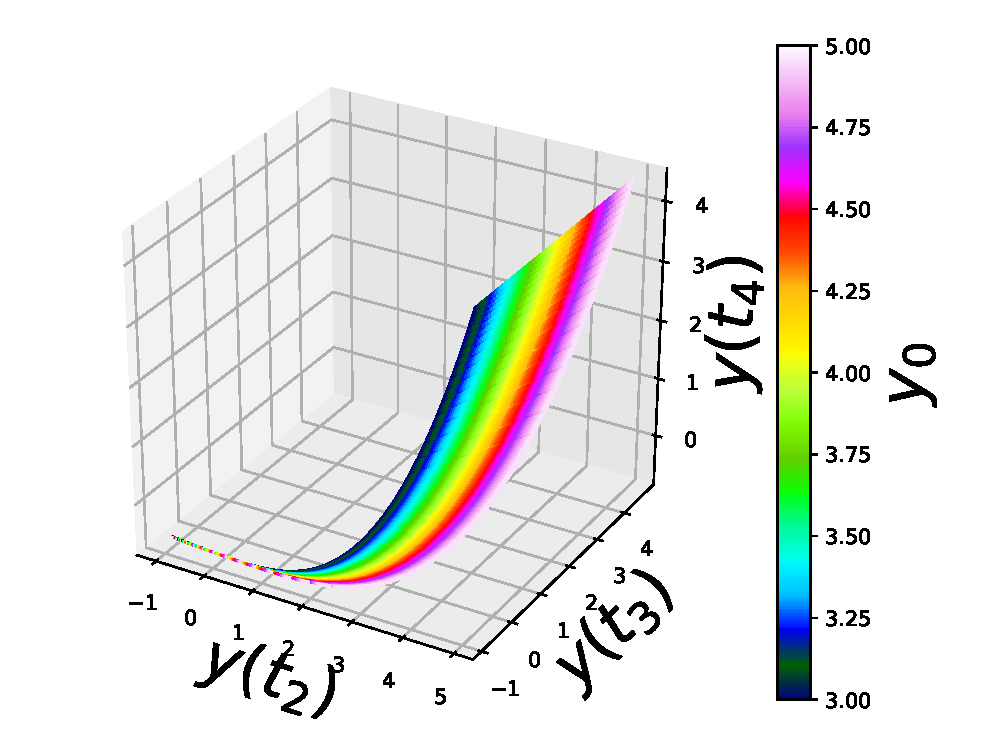
\includegraphics[width=0.33\textwidth]{mod_man_y0} &
                                                                                                                    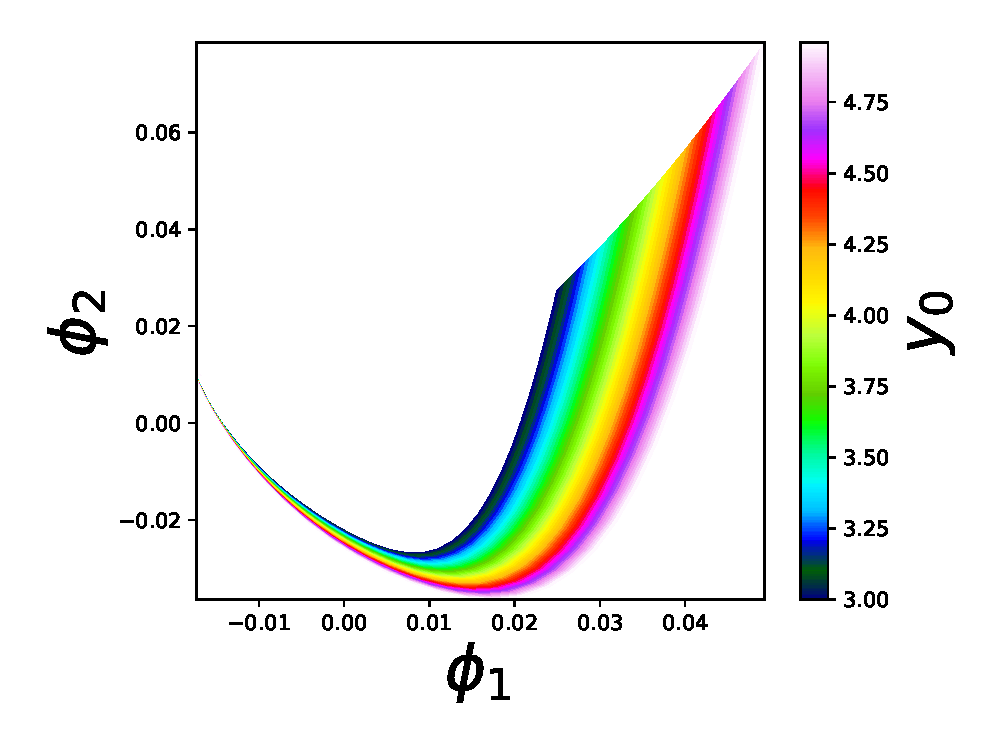
\includegraphics[width=0.33\textwidth]{phi2_phi1_y0_sing}  \\
    (d) & (e) & (f)\\
  \end{tabular}
  \caption[DMAPS results for singularly perturbed system]{(a) and (d) Parameter space colored by $\phi_1$ and
    $\phi_2$; (b) and (e) Model manifold colored by $\epsilon$ and
    $y_0$; (c) and (f) Diffusion map space colored by $\epsilon$ and
    $y_0$ \label{fig:singpert-dmaps}}
\end{figure}


\begin{figure}[!htp]
  \centering
  \begin{tabular}{c}
    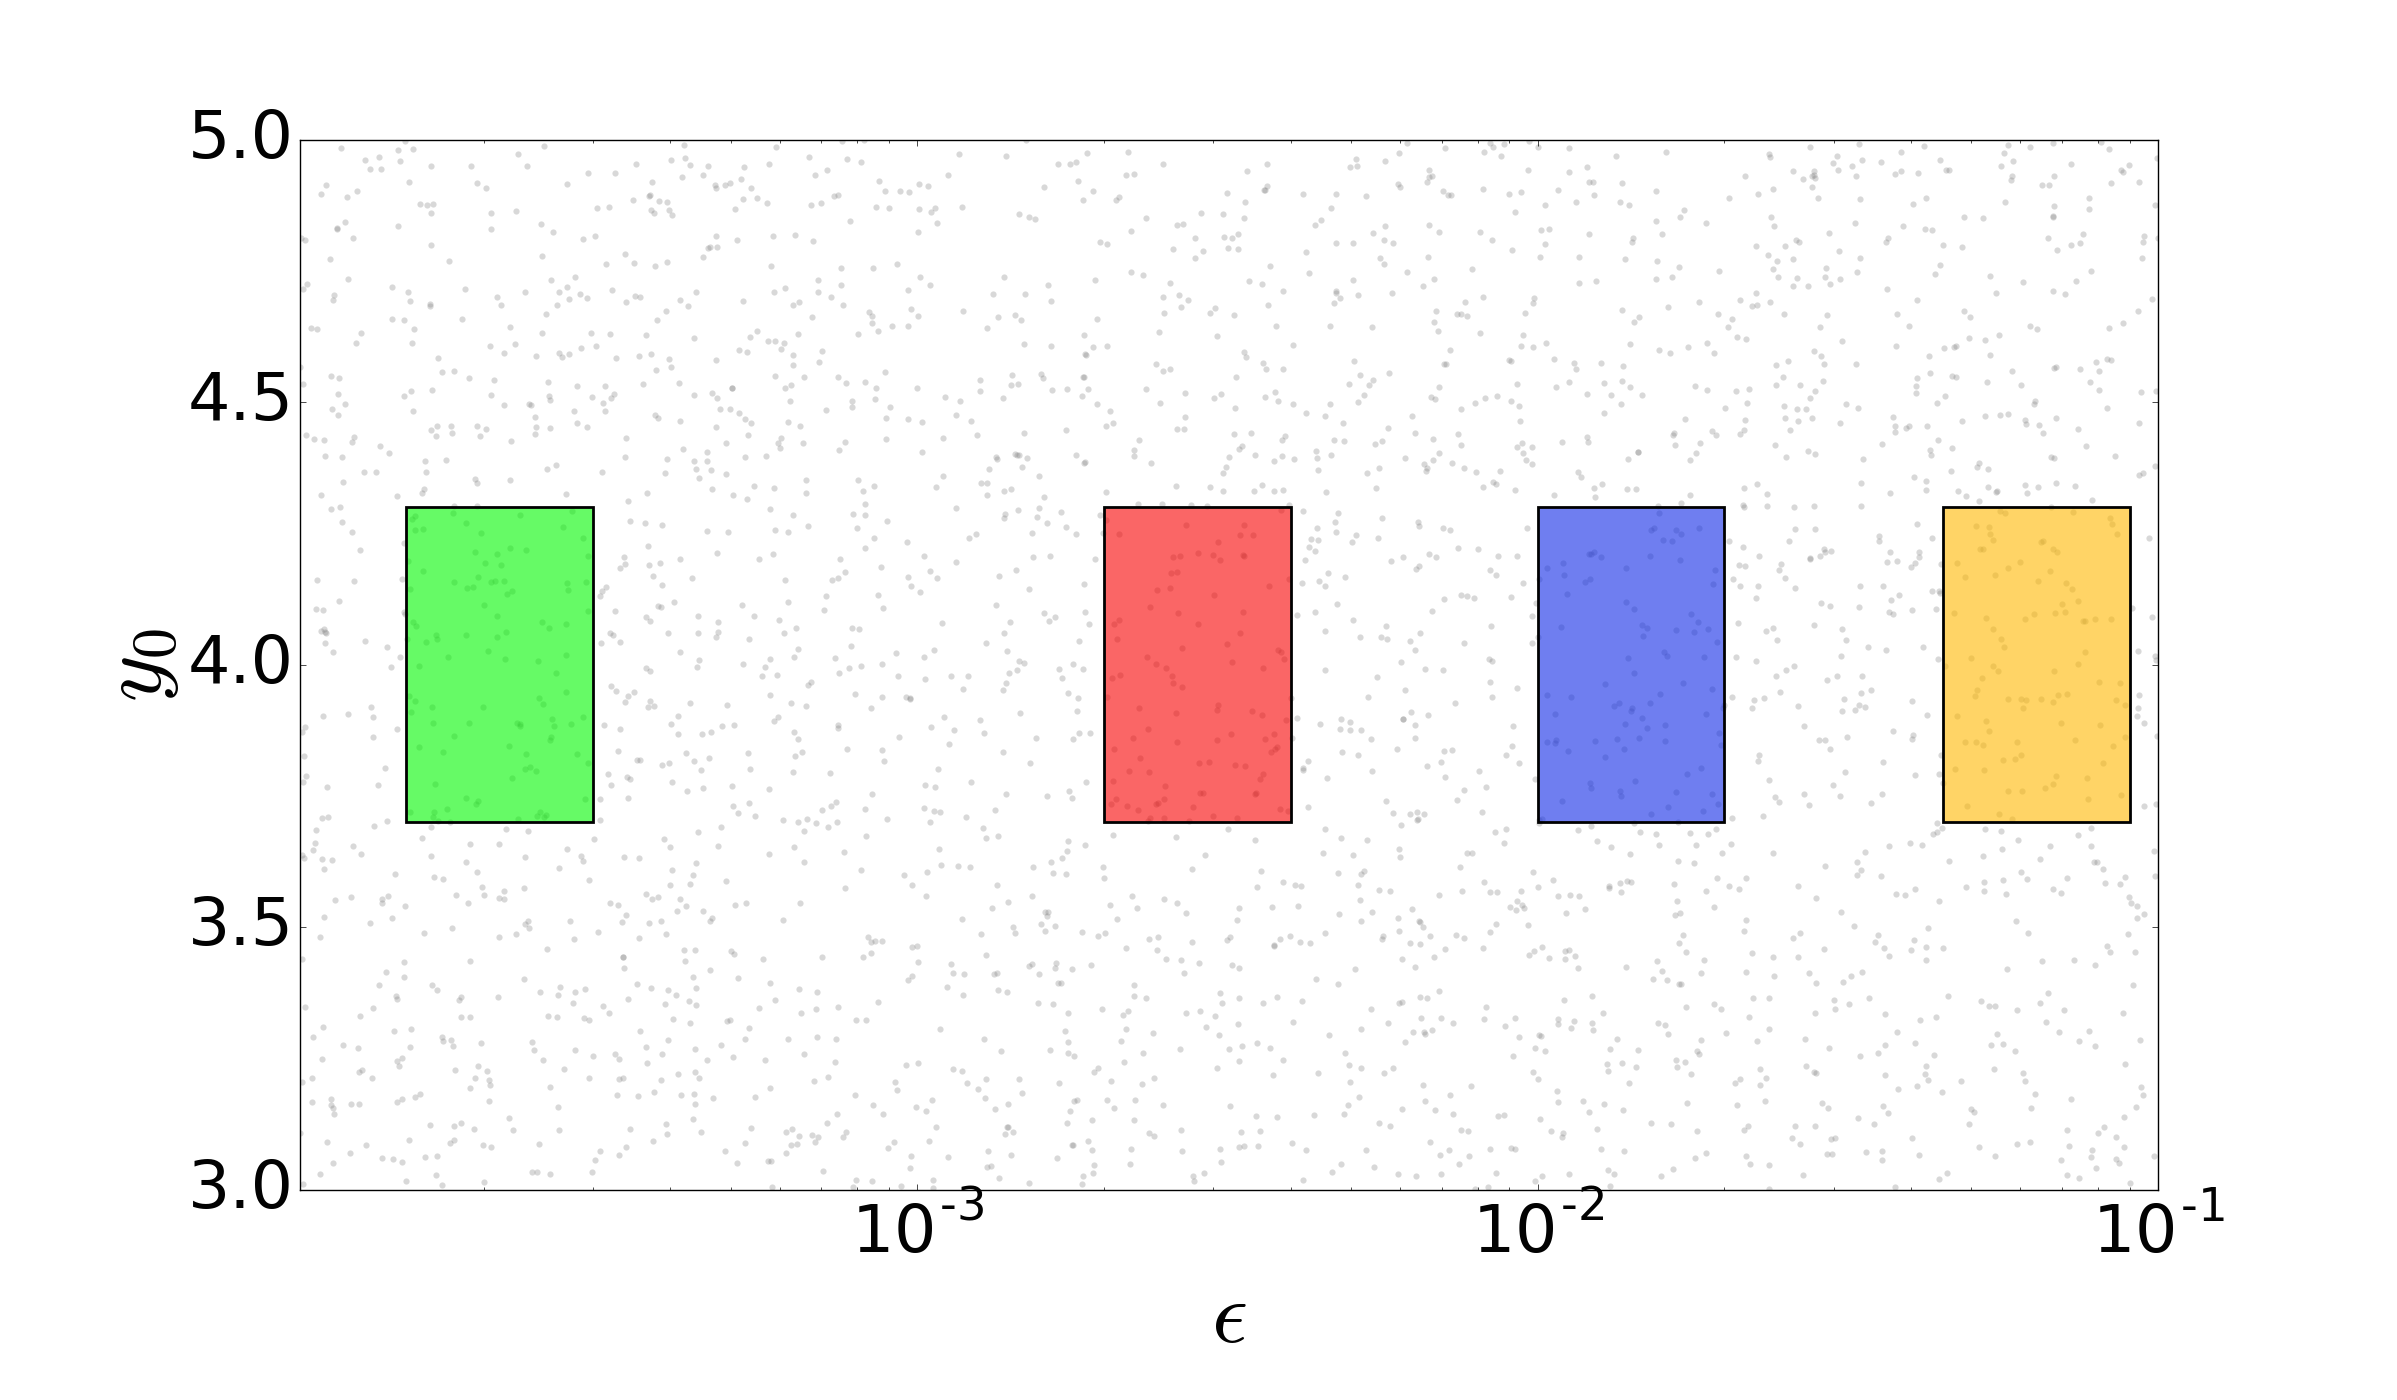
\includegraphics[height=0.2\textheight]{y0-eps-patches} \\
    (a)\\
    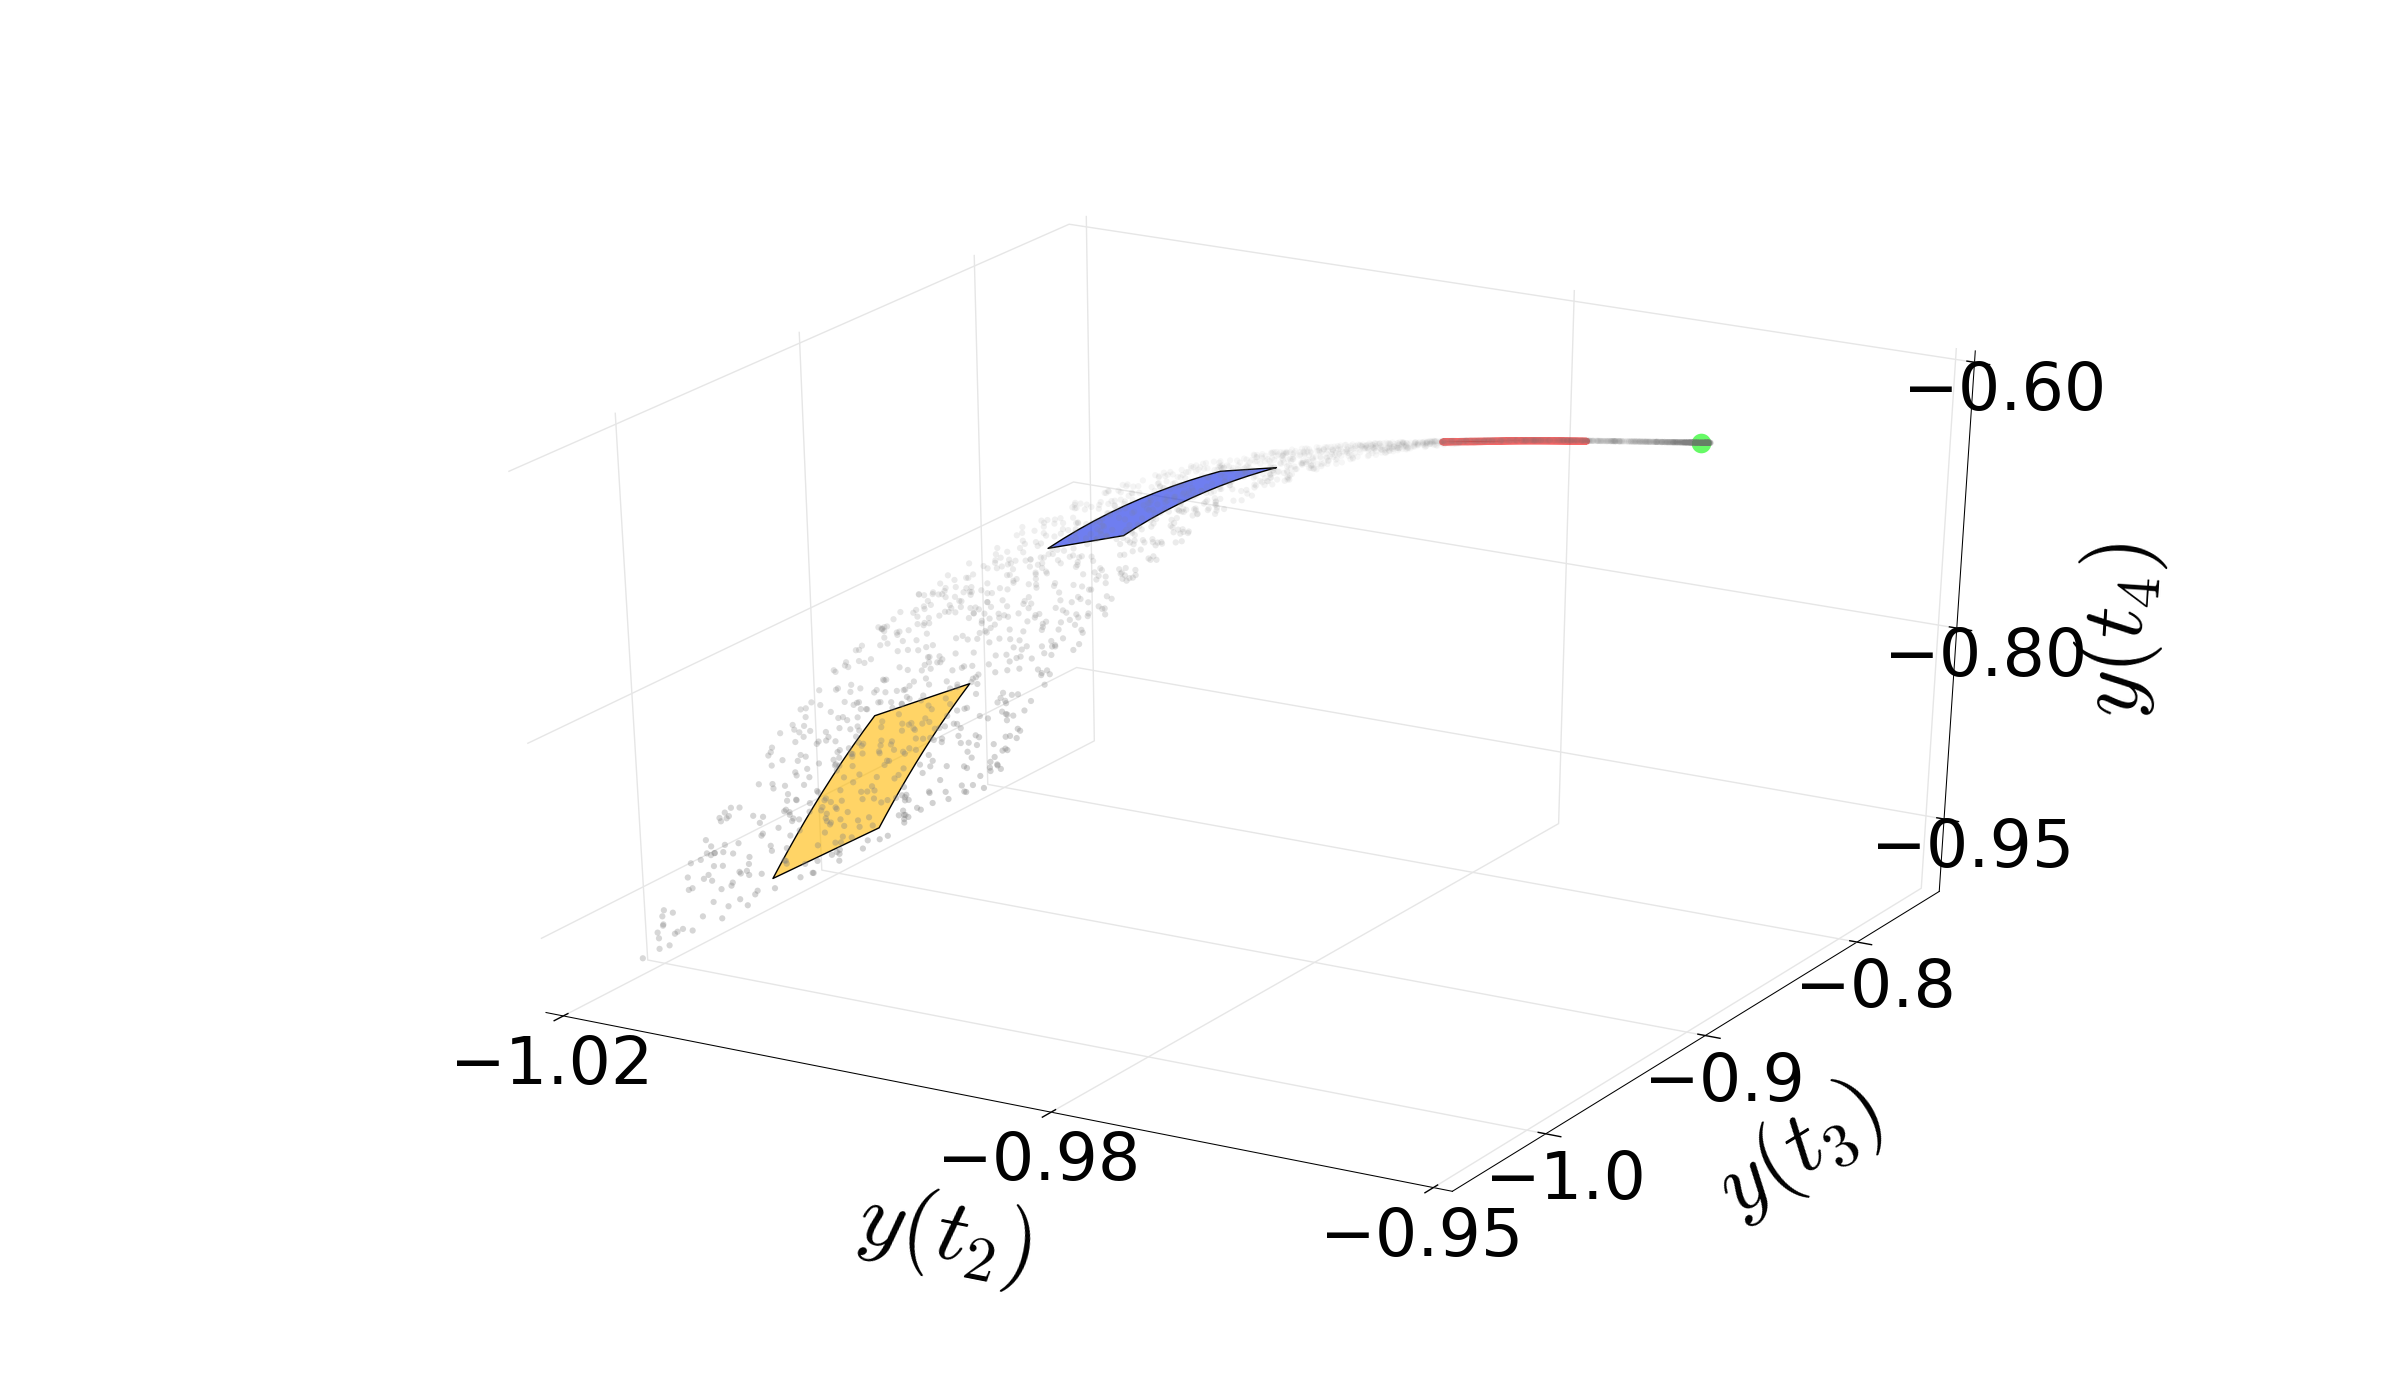
\includegraphics[height=0.2\textheight]{y4-y3-y2-patches}\\
    (b)\\
    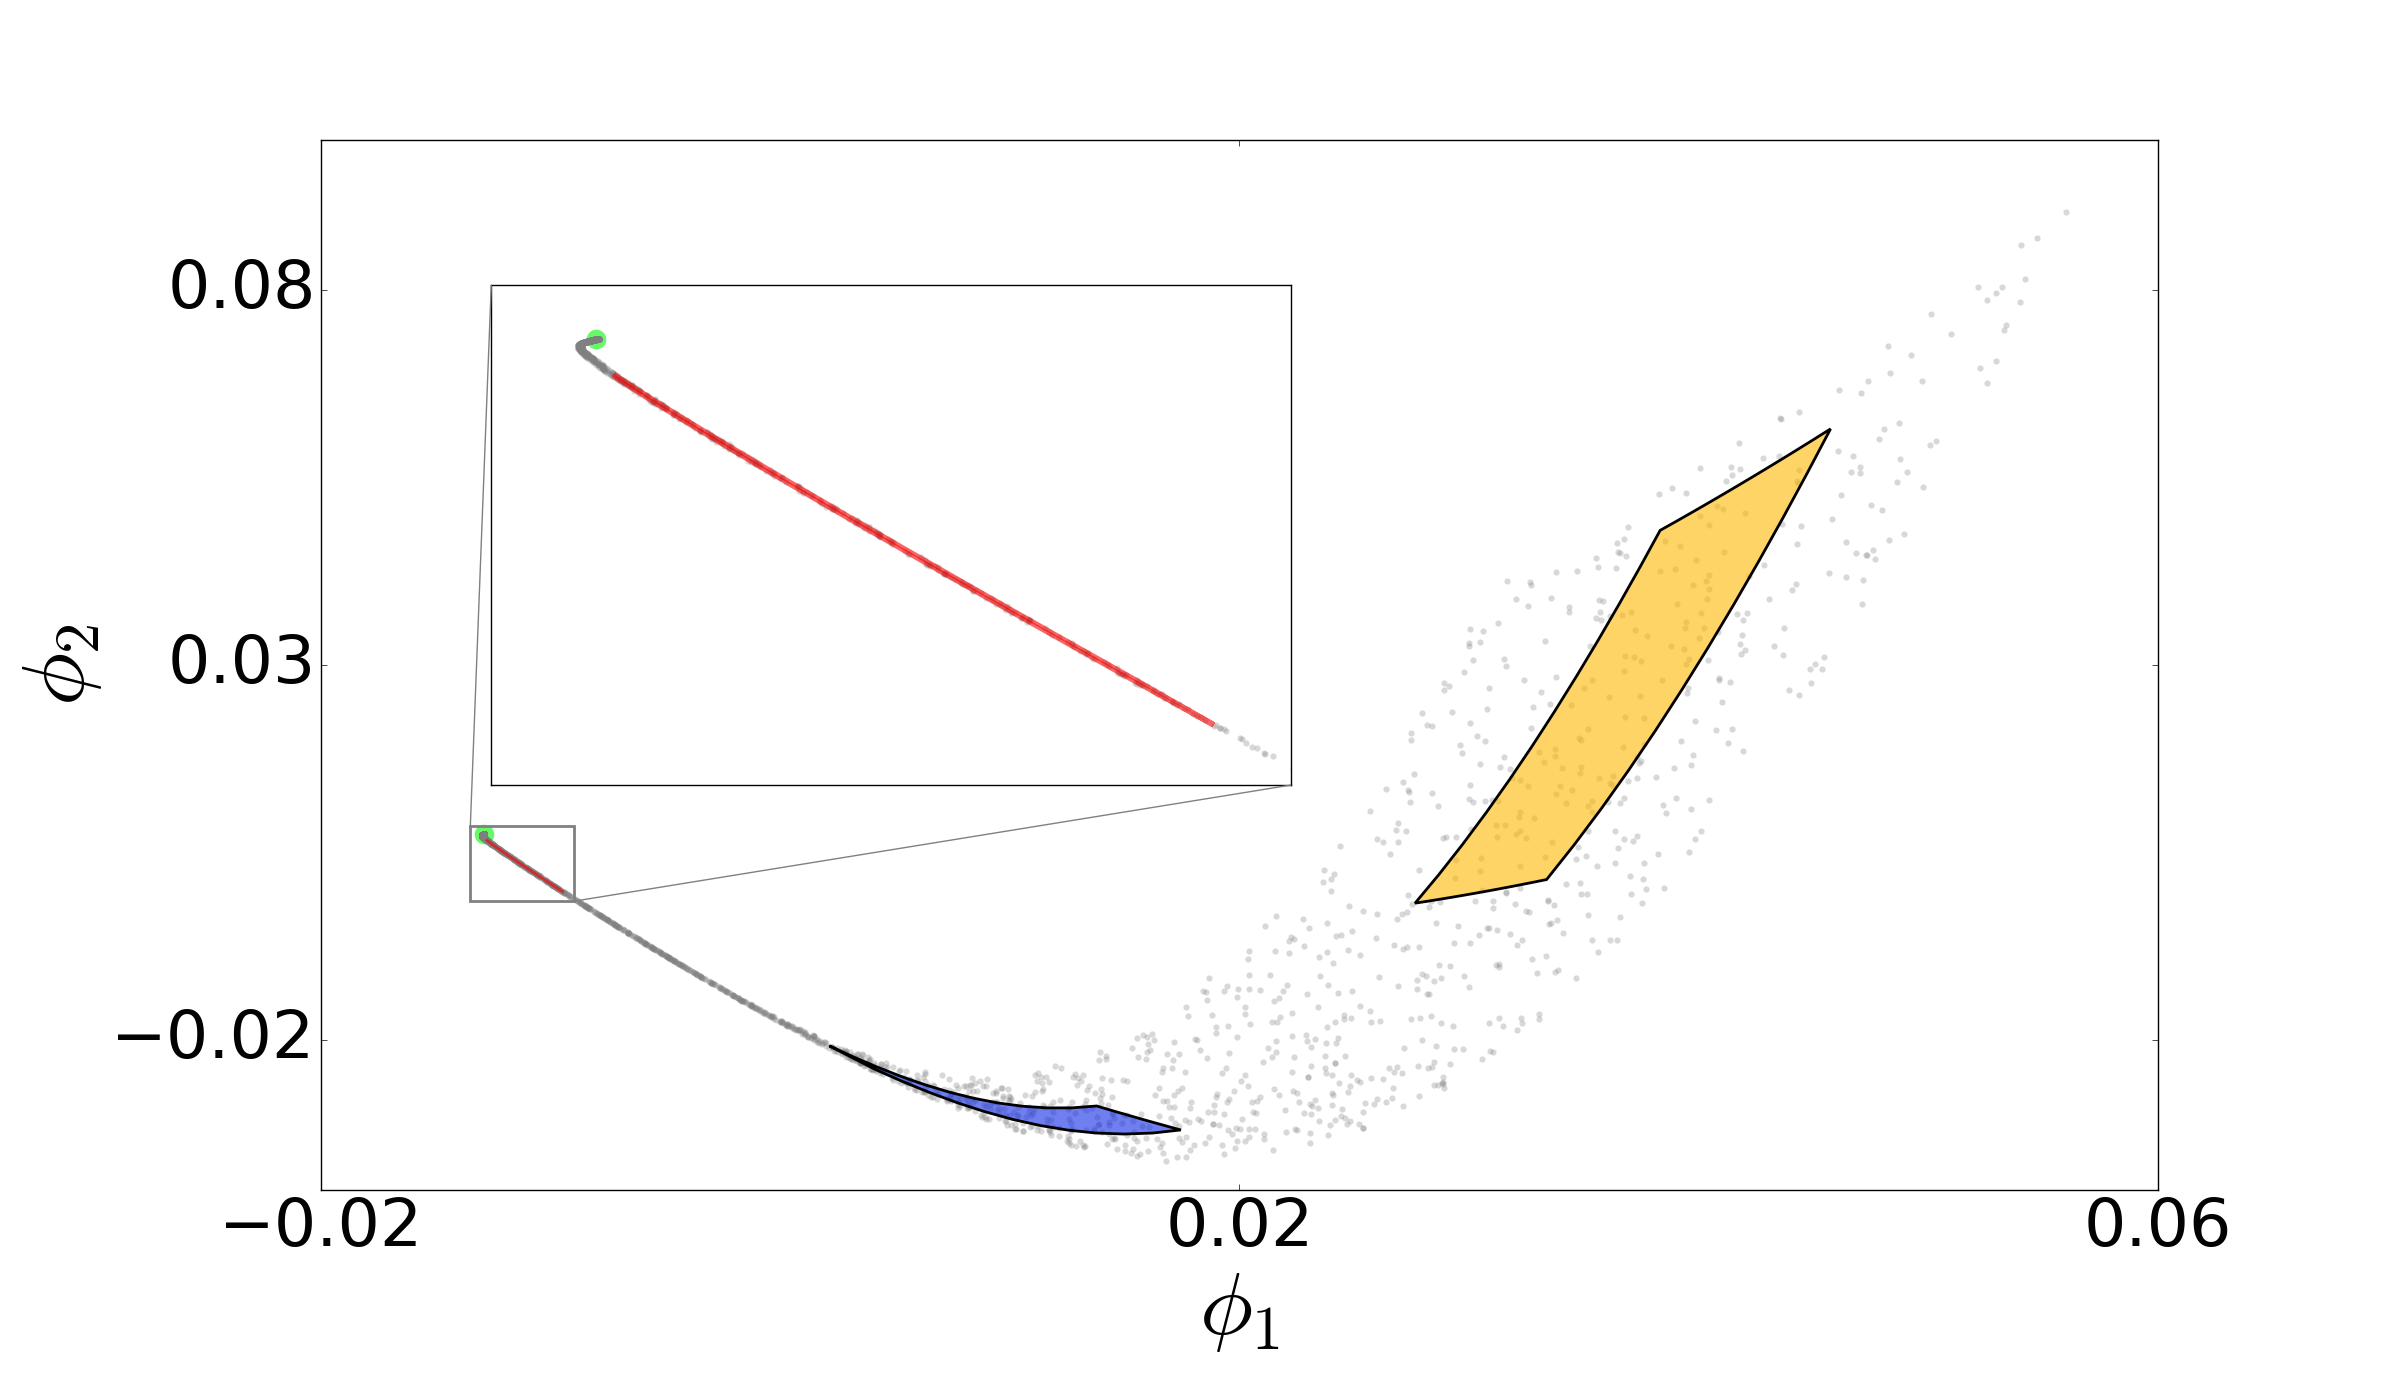
\includegraphics[height=0.2\textheight]{phi2-phi1-patches}\\
    (c)\\
  \end{tabular}
  \caption[Different views of singularly perturbed system]{(a) Patches in parameter space for the singularly perturbed
    system; (b) Corresponding patches in model response space; (c)
    Corresponding patches in DMAPS embedding
    space \label{fig:singpert-patches}}
\end{figure}


\section{Application to Michaelis-Menten kinetics}

Finally, we apply our toolbox to a familiar chemical kinetic
prototype, namely the Michaelis-Menten system modeling enzymatic
action \cite{johnson_original_2011}.  In that mechanism, a substrate
$S$ is turned into product $P$ by the action of an enzyme $E$ through
the creation of an intermediate complex $C$,

\begin{align}
  E + S \xrightleftharpoons[k_{-1}]{k_1} C \xrightarrow[]{k_2} E + P
  \label{mech:mm}
\end{align}

The mechanism differs from Mechanism~\ref{mech:abc} in that the
addition of a recycled but limited enzyme supply introduces
nonlinearities into the governing system of differential equations,


\begin{align}
  \begin{split}
    S' &= -k_1 E S + k_{-1} C , \\
    C' &= k_1 E S - (k_{-1} + k_2) C , \\
    E' &= -k_1 E S + (k_{-1} + k_2) C , \\
    P' &= k_2 C
  \end{split}
\end{align}


The conservation laws $S + P + C = S_T$ and $E + C = E_T$ reduce the
number of variables by two, and we arrive at the final model

\begin{align}
  \begin{split}
    S' &= -k_1 (E_T-C) S + k_{-1} C , \\
    C' &= k_1 (E_T-C) S - (k_{-1} + k_2) C
    \label{eq:MM}
  \end{split}
\end{align}

Following the classical setting
\cite{johnson_original_2011,johnson_original_2011,segel_quasi-steady-state_1989},
we set the initial concentrations of complex and product to zero,
$C_0=P_0=0$, so that $S_0 = S_T$ and $E_0 = E_T$.  Further adapting
ideas from \cite{segel_quasi-steady-state_1989}, we recoordinatize the
parameter space through the transformations

\begin{align}
  \begin{split}
    K_M = \dst\frac{k_{-1} + k_2}{k_1} , &\quad
    V_M = k_2 E_T , \\
    \sigma = \dst\frac{S_T}{K_M} , \quad \kappa =
    \dst\frac{k_{-1}}{k_2} , &\quad \epsilon = \dst\frac{E_T}{S_T +
      K_M}
    \label{eq:param-defs}
  \end{split}
\end{align}

The observable here is the product concentration $P$ at ten equally
spaced times in the interval $[t_s/2,2t_s]$, where the timescale
$t_s = (S_T^* + K_M^*)/V_M^*$. Thus
$f:\mathbb{R}^5 \rightarrow \mathbb{R}^{10}$ maps our five
parameter values to ten points along $P$'s trajectory. Setting
reference parameter values at
$(K_M^*,V_M^*,S_T^*,\epsilon^*,\kappa) = (1,1,1,10^{-3},10)$, we
investigate the system in a manner similar to that previously
presented.  First we sample parameter settings lying within a fixed
distance $\delta=0.05$ of
$f^* = f(K_M^*, V_M^*, S_T^*, \epsilon^*,
\kappa^*)$, and then we apply the modified DMAPS algorithm to that
dataset to uncover significant parameter combinations.  Before delving
into DMAPS, however, we first probe the system with a simpler, linear
PCA analysis.  By applying this technique to the Jacobian of the model
response

\begin{align}
  \mathrm{J} = \begin{bmatrix} \frac{\partial f_1}{\partial K_M} &
    \frac{\partial f_1}{\partial V_M} & \frac{\partial f_1}{\partial
      S_T} & \frac{\partial f_1}{\partial \epsilon} & \frac{\partial
      f_1}{\partial \kappa} \\ \vdots & & & & \vdots \\ \frac{\partial
      f_N}{\partial K_M} & & \hdots & & \frac{\partial f_N}{\partial
      \kappa} \end{bmatrix}
\end{align}

and examining the coefficients of the principal components
$\mathrm{V}$ where $\mathrm{J} = \mathrm{U \Sigma V^T}$, we will
uncover, in a local, linear sense, a basis for parameter space which
better captures the directions which do and do not affect model
output. This can be observed from the fact that
$\| f(\theta + \Delta \theta) - f(\theta) \| \approx \| \mathrm{J}
\Delta \theta \| = \| \mathrm{U \Sigma V^T} \Delta \theta
\|$. When $\Delta \theta$ aligns with a principal component whose
corresponding singular value is large, it will point in a direction of
significant model response variation. Conversely, a
$\Delta \theta$ which aligns with a principal component whose
singular value is small will point in a sloppy direction along which
model response changes minimally. Examining the SVD of the Jacobian
evaluated at $\theta^*$ we find for the principal components (with
entries less than $10^{-1}$ rounded to zero and singular values
rounded to the nearest order of magnitude for clarity)

\[
  V = \begin{blockarray}{cccccc} & v_1 & v_2 & v_3 & v_4 & v_5
    \\ \begin{block}{c[ccccc]} K_M & 0.3 & \minus 0.4 & \minus 0.9 & 0
      & 0 \\ V_M & \minus 0.4 & 0.8 & \minus 0.5 & 0 & 0 \\ S_T &
      \minus 0.9 & \minus 0.5 & 0 & 0 & 0 \\ \epsilon & 0 & 0 & 0 &
      0.9 & \minus 0.5 \\ \kappa & 0 & 0 & 0 & \minus 0.5 & \minus 0.9
      \\ \end{block} & & & & & \\ \begin{block}{c[ccccc]} \sigma &
      10^0 & 10^0 & 10^{\minus 2} & 10^{\minus 5} & 10^{\minus 6}
      \\ \end{block} \end{blockarray}
\]

where the final row labeled $\sigma$ contains the corresponding
singular values. This simple analysis immediately suggests the
existence of two sloppy parameters in this regime, $\kappa$ and
$\epsilon$, as the principal components that span these axes
correspond to significantly smaller singular values compared to the
other vectors. In addition, it appears that the parameter space
direction $K_M = V_M$ may be sloppy as this approximately corresponds
to the third smallest principal component, singular value pair. With
this simple analysis in hand, we turn to computational verification of
the results using both direct numerical experiments and the DMAPS
scheme outlined above, along with supporting analytical arguments.

First we show that the direction $K_M = V_M$ is indeed sloppy so that
one cannot precisely determine both $K_M$ and $V_M$, but only their
ratio. To do so we turn to the Lineweaver-Burk plot, a graphical
procedure allowing one to determine $K_M$ and $V_M$ from experimental
data of the reaction rate and substrate concentration evolution over
time \cite{lineweaver_determination_1934}. By generating many noisy realizations of the product
concentration profiles as one might collect experimentally in the lab
and then fitting each with the Lineweaver-Burk method, we can observe
the range of predicted $K_M$, $V_M$ pairs. These results are plotted
in Fig.~\ref{fig:lb}. In a typical setting we would expect a spread of
predicted values centered around the true, zero-noise parameters
taking the shape of some ellipsoid. However, as we have seen in
previous examples, in the presence of sloppiness this ellipsoid would
be stretched out along the sloppy parameter direction. This is
precisely what we find in Fig.~\ref{fig:lb}: so long as the ratio
$K_M/V_M = K_M^*/V_M^* = 1$, a wide range of values provide best-fit
parameters in the presence of slight noise. Therefore, when fitting
parameters in this regime, we must accept that we may not be able to
determine precise values of both $K_M$ and $V_M$.


\begin{figure}
  \centering
  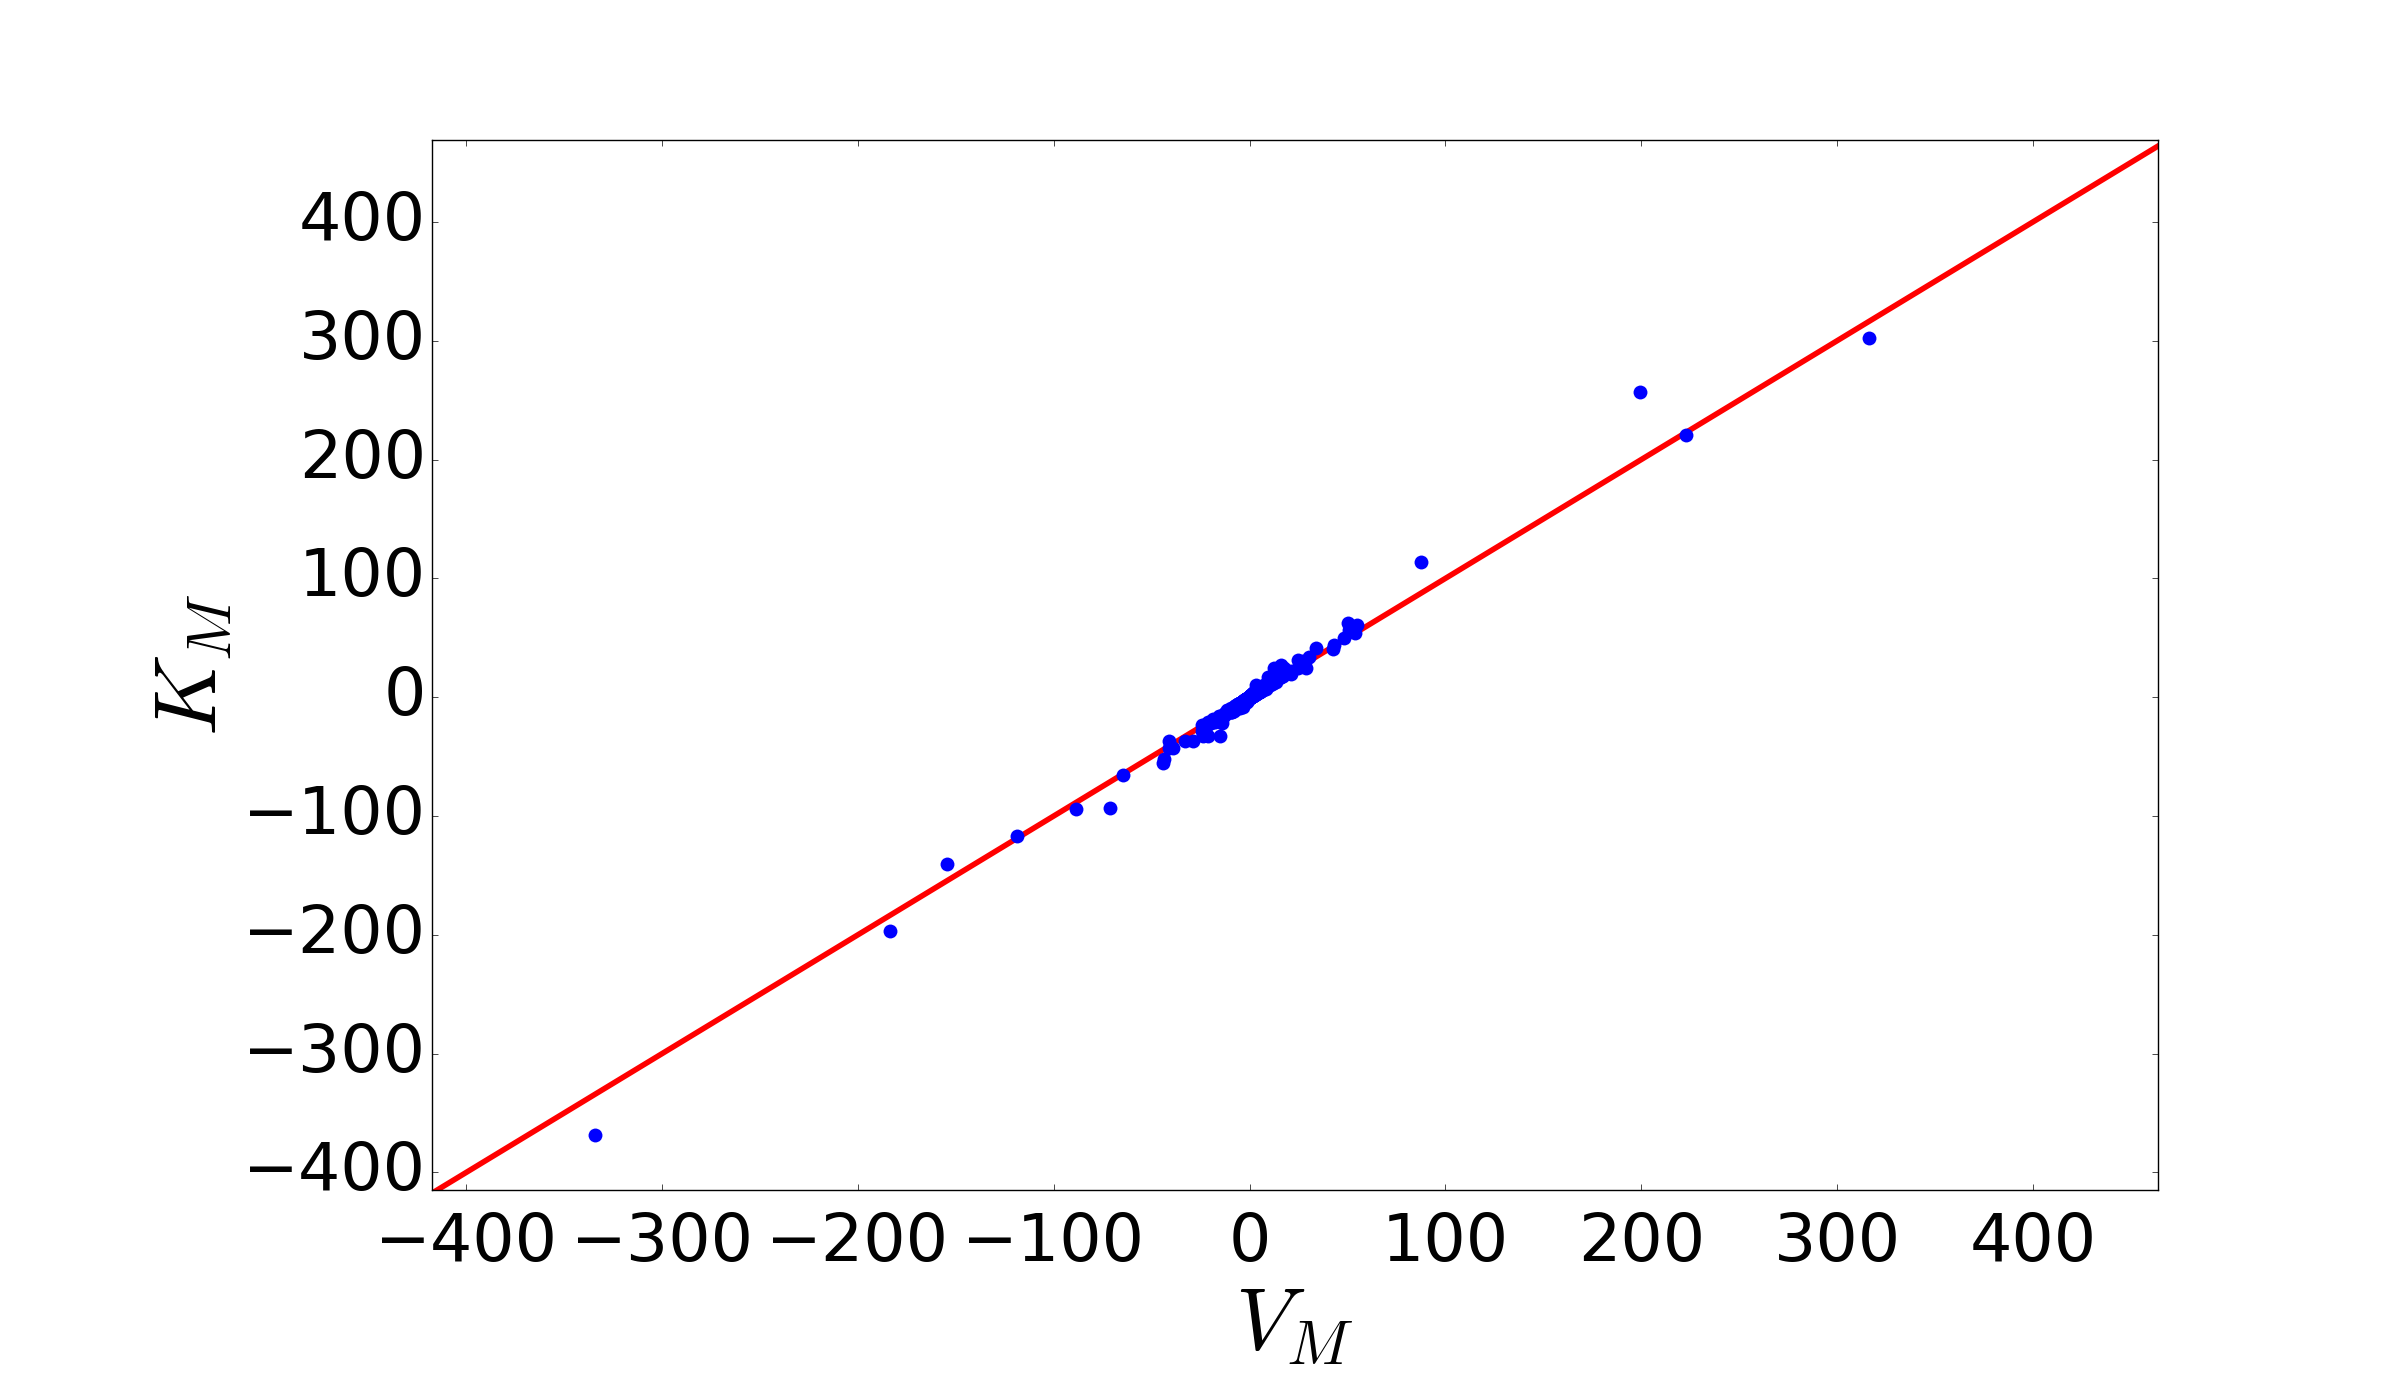
\includegraphics[width=1.0\linewidth]{k-v-lb}
  \caption[Lineweaver-Burk fitting results]{Best fit $K_M$ and $V_M$ values for many noisy
    concentration trajectories (blue dots). Sloppiness is evident in
    the spread of the data along the line $K_M/V_M = 1$ (plotted in
    red for reference). \label{fig:lb} }
\end{figure}

Next, we examine the system using DMAPS. We use the five-dimensional
dataset obtained by sampling parameter space around $\theta^*$ and
keeping those points for which
$\|f(\theta) - f(\theta^*) || < 5 \cdot 10^{-2}$, and apply DMAPS
with an $\epsilon$ value of $10^{-1}$.

Having computed our DMAP eigenvectors, it remains to determine which
of them correspond to independent directions in parameter space, as
certain eigenvectors may parameterize the same directions (see
\cite{dsilva_parsimonious_2015} for details). Using the algorithm
developed in \cite{dsilva_parsimonious_2015}, we compute a residual
for each eigenvector which, roughly speaking, assesses how much new
information it contains. The results shown in Fig~\ref{fig:resids}
suggest that eigenvectors $\phi_1$ and $\phi_2$ parameterize
independent directions. Our previous analysis would then suggest that
$\phi_1$ and $\phi_2$ correspond to important parameter directions,
and would provide a good set of coordinates on our model manifold.

We can test this hypothesis by projecting the model manifold onto two
axes, here $f_1$ and $f_{10}$, and coloring the result by our
eigenvectors. If the colors vary smoothly over the points, we have
uncovered an eigenvector that parameterizes the manifold. These
colorings are provided in Fig.~\ref{fig:mm-dmaps}. Based on these
figures, we can conclude that indeed $\phi_1$ and $\phi_2$ provide
coordinates along the model manifold. The sloppiness in $K_M/V_M$ was
discussed in the previous paragraph, but it remains to show why we
would lose two more parameters. In fact, as $\epsilon \rightarrow 0$,
the set of differential equations given in \eqref{eq:MM} become
singularly perturbed. In this limit, the leading order dynamics are
not influenced by $\kappa$, as shown in
\cite{segel_quasi-steady-state_1989}. Thus, for small enough
$\epsilon$, we will lose our ability to determine both $\epsilon$ and
$\kappa$. This is precisely what is reflected in our DMAPS results.

\begin{figure}[!htp]
  \centering
  \begin{tabular}{cc}
    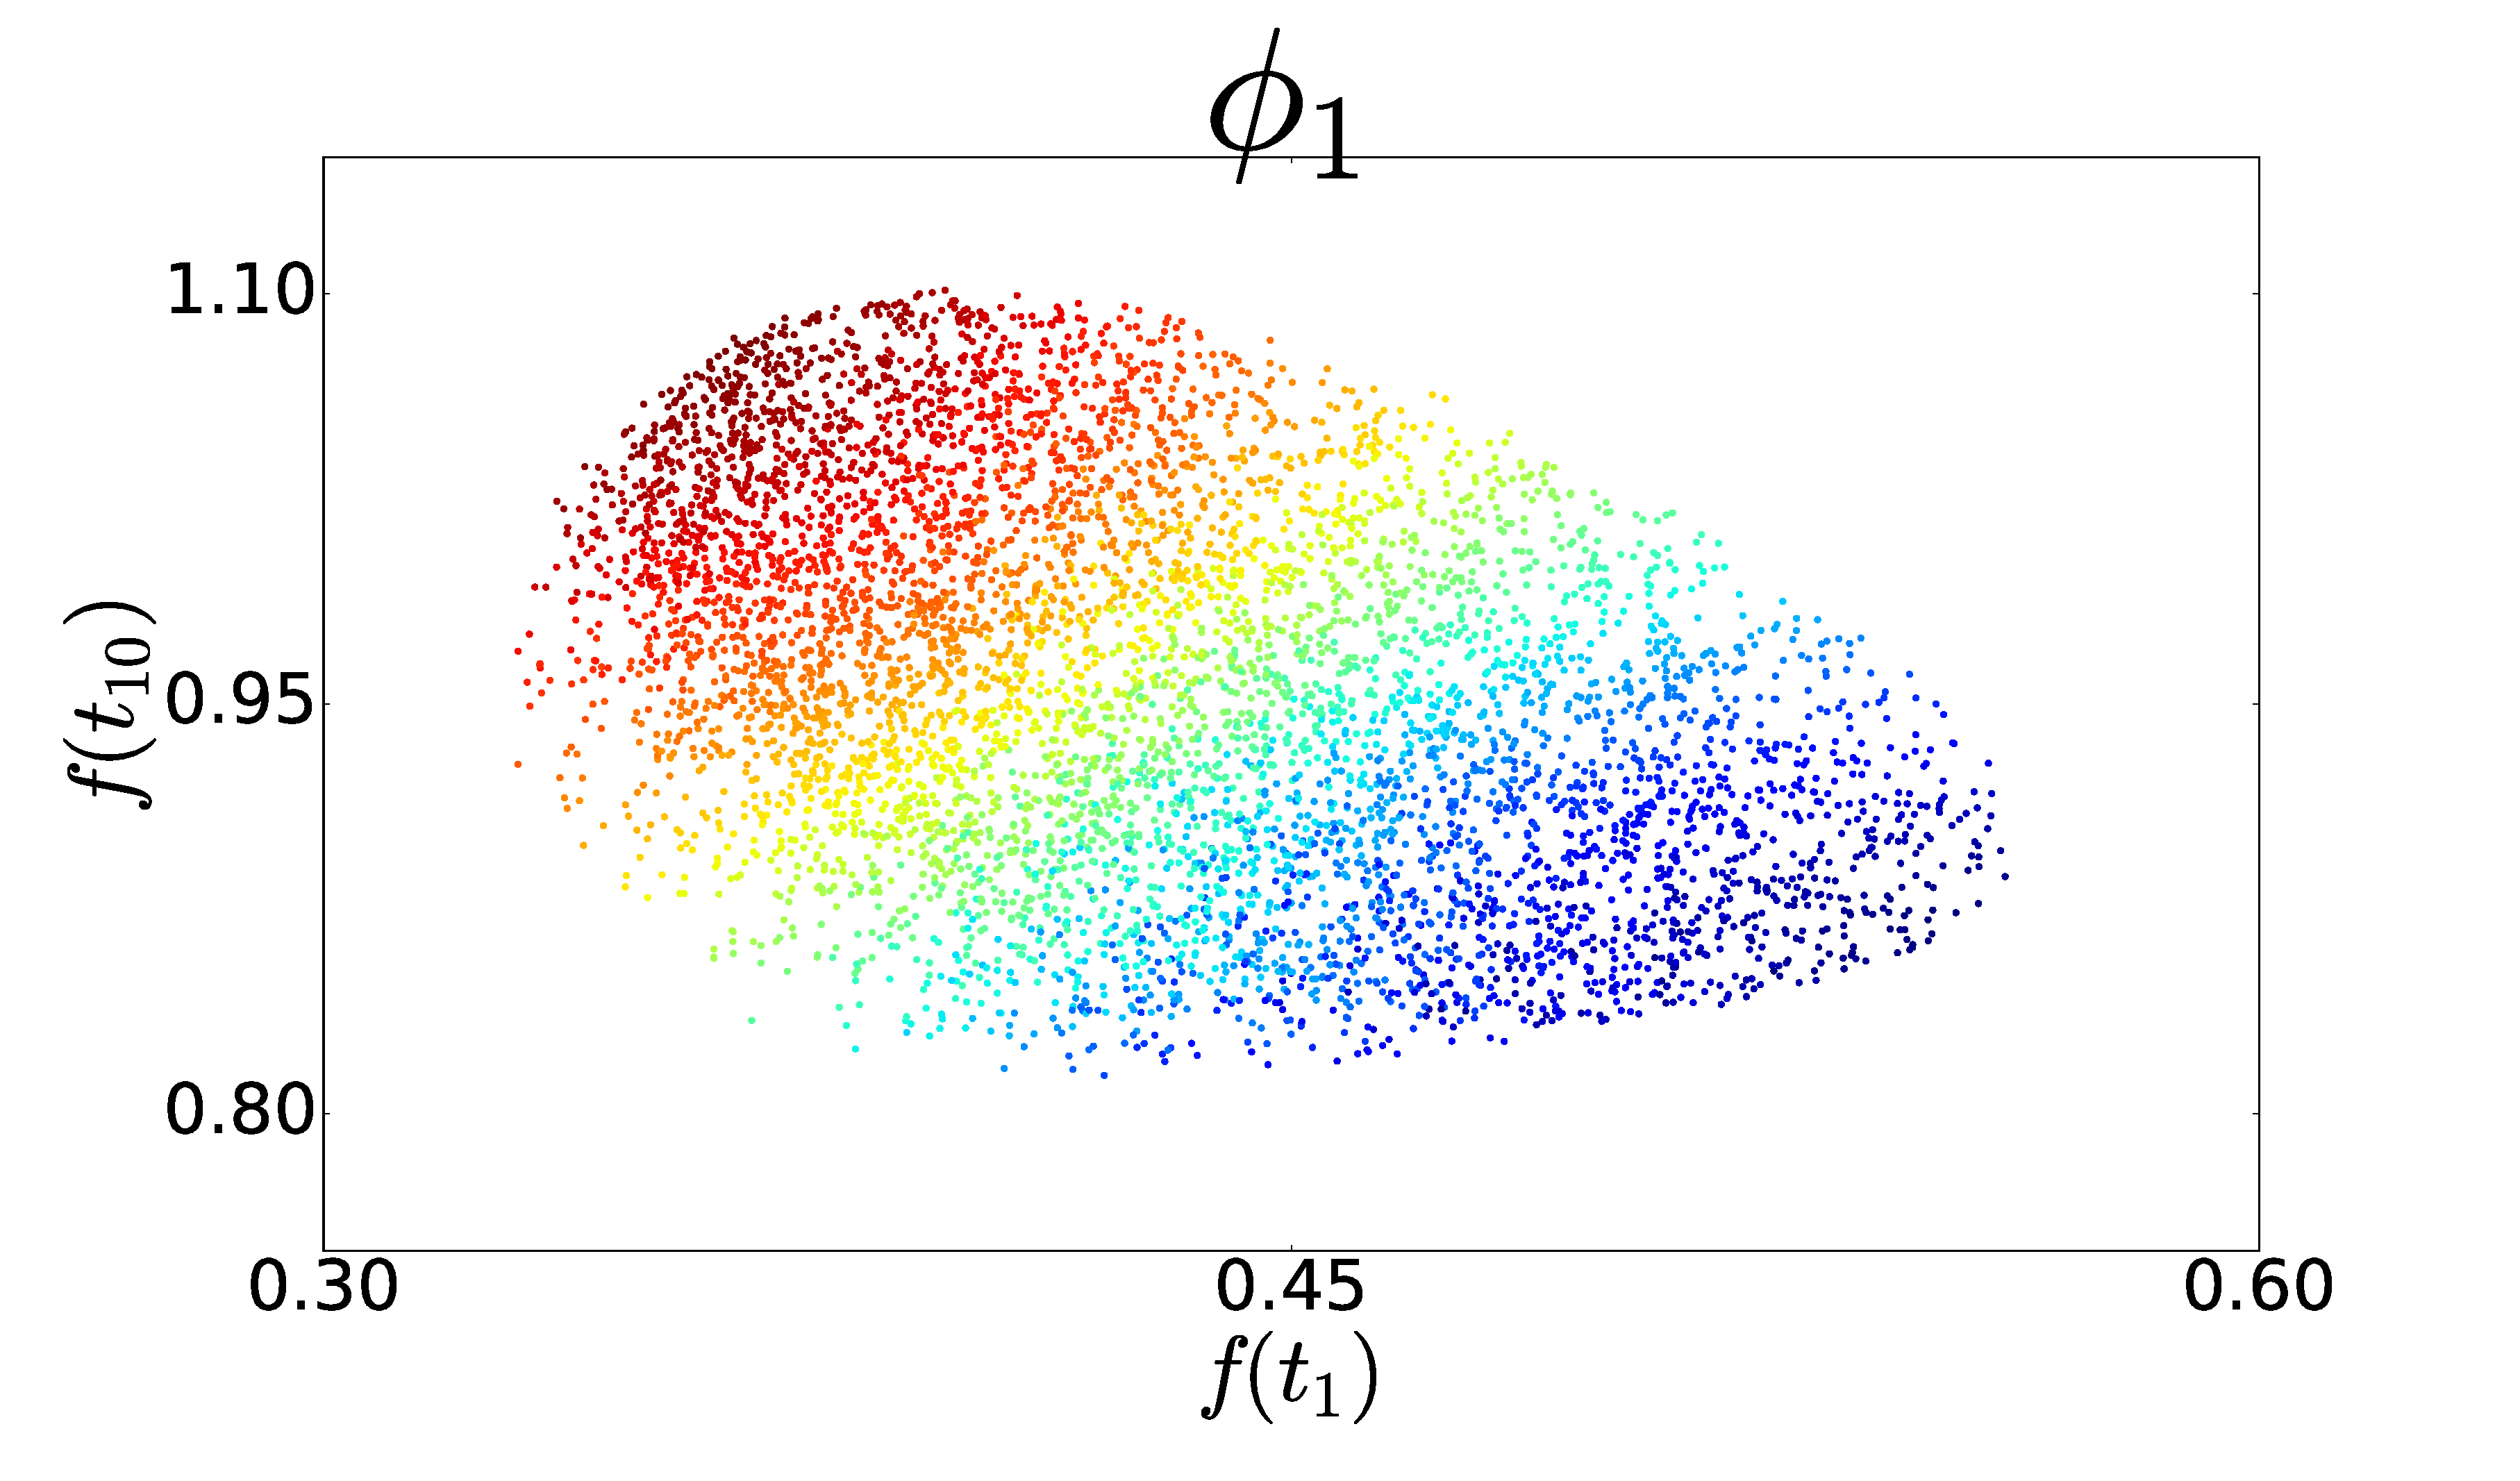
\includegraphics[width=0.5\textwidth]{f10-f1-phi1} &
    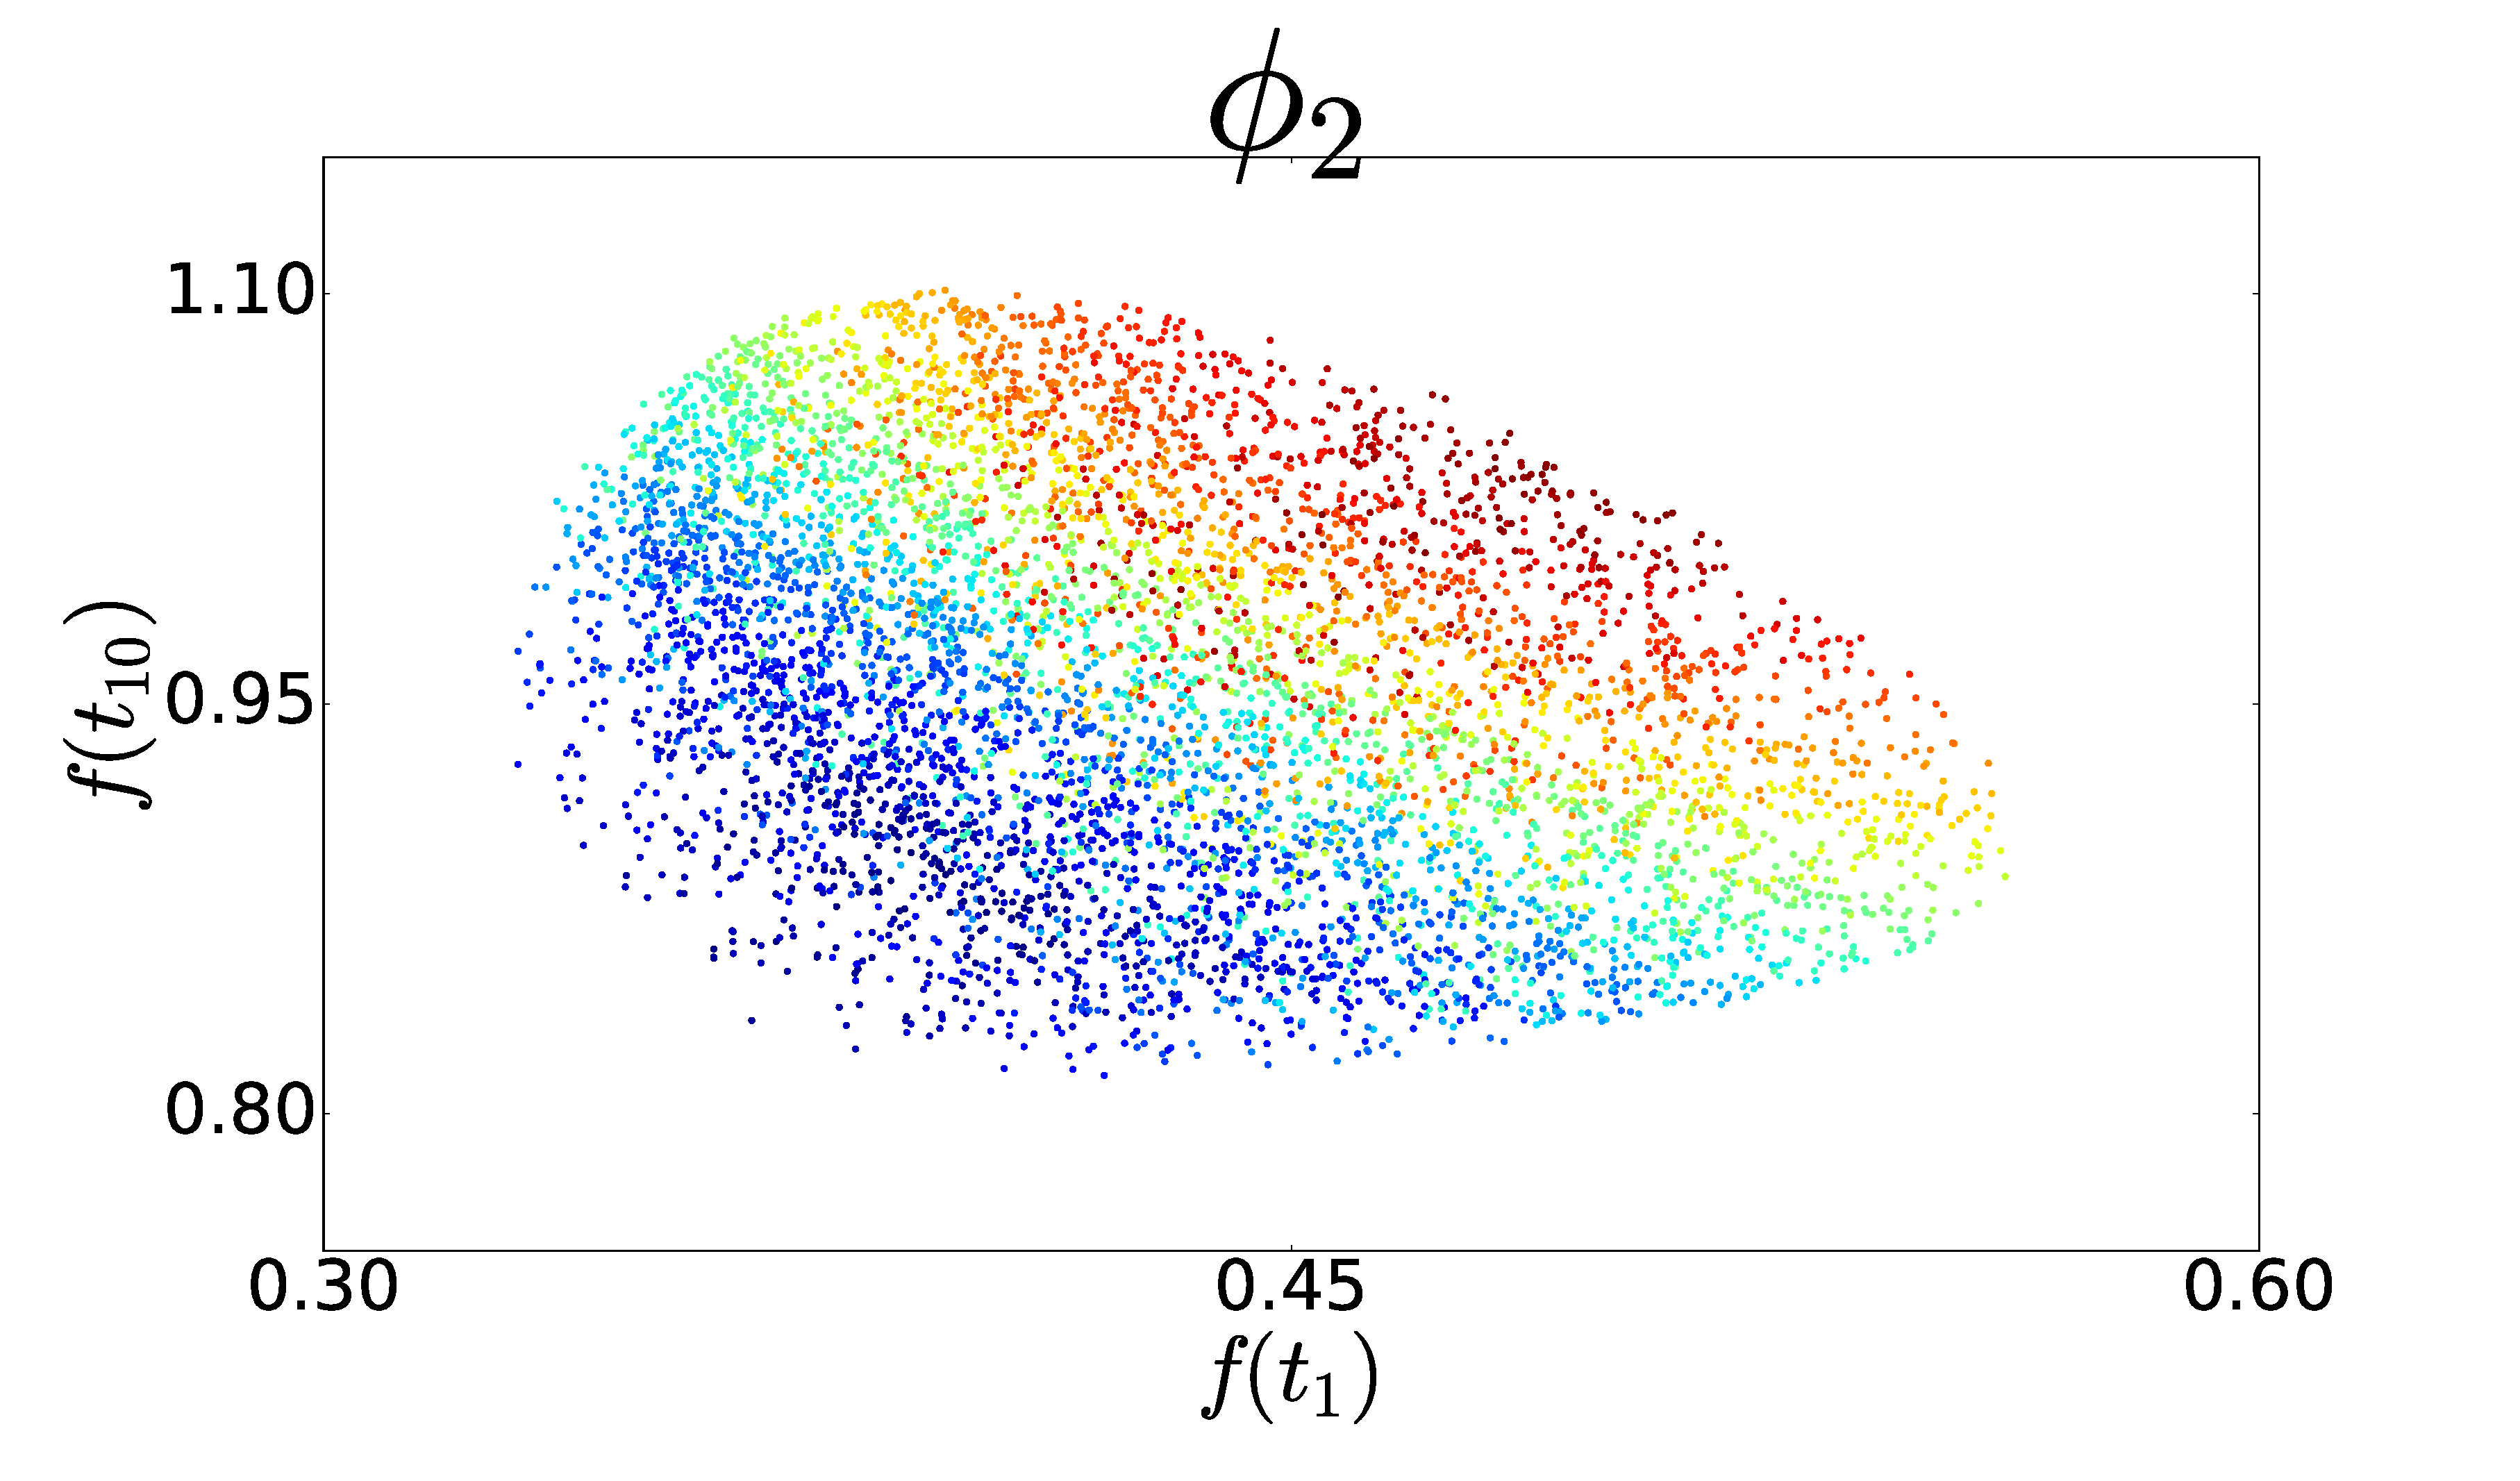
\includegraphics[width=0.5\textwidth]{f10-f1-phi2}\\
    (a) & (b) \\
  \end{tabular}
  \caption[DMAPS results for Michaelis-Menten system I]{Projection of the model manifold onto $f_1$ and $f_{10}$
    colored by different DMAP eigenvectors. As $\phi_1$ and $\phi_2$
    vary smoothly over the surface and parameterize independent
    directions, these eigenvectors offer a good pair of coordinates on
    the manifold \label{fig:mm-dmaps}}
\end{figure}


\begin{figure}[ht!]
  \centering
  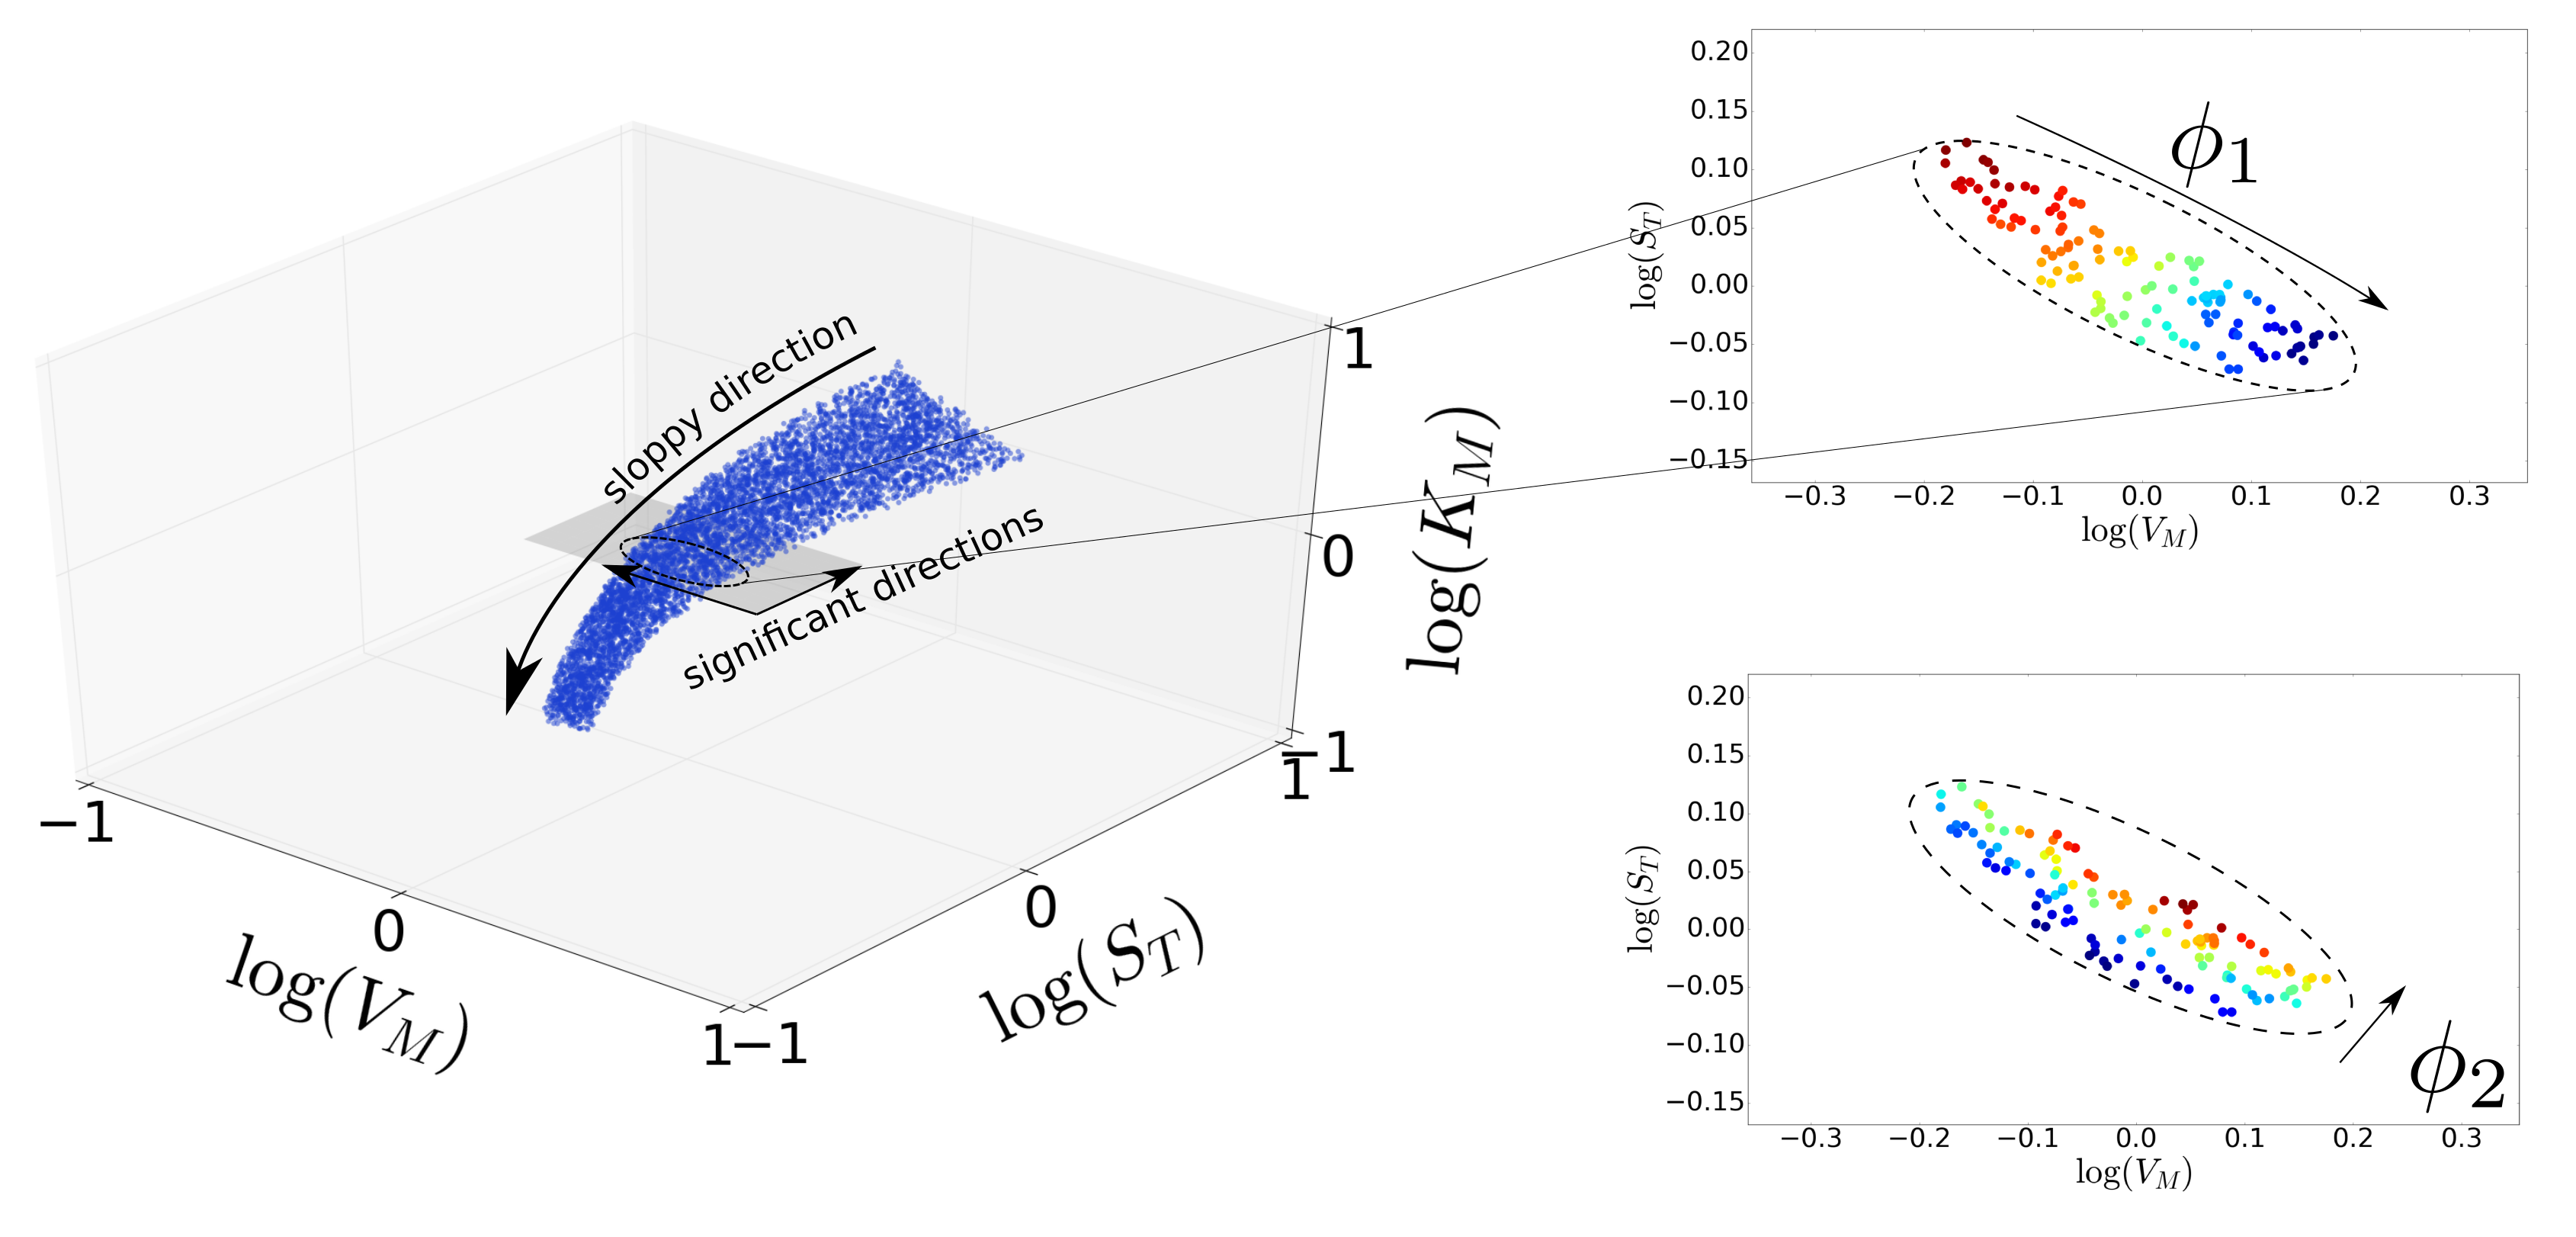
\includegraphics[width=\textwidth]{vm-st-km-all}
  \caption[DMAPS results for Michaelis-Menten system II]{(left) Scatter-plot of points in parameter space such that
    $\|f(\theta) - f^*\| < \delta$. This reveals a sloppy direction
    corresponding to the long, curved axis, and two significant
    directions orthogonal to it. (right) Two-dimensional cross section
    colored by $\phi_1$ and $\phi_2$. As expected, these eigenvectors
    do parameterize the significant directions in parameter space.
    \label{fig:mm-all} }
\end{figure}

\begin{figure}
  \centering
  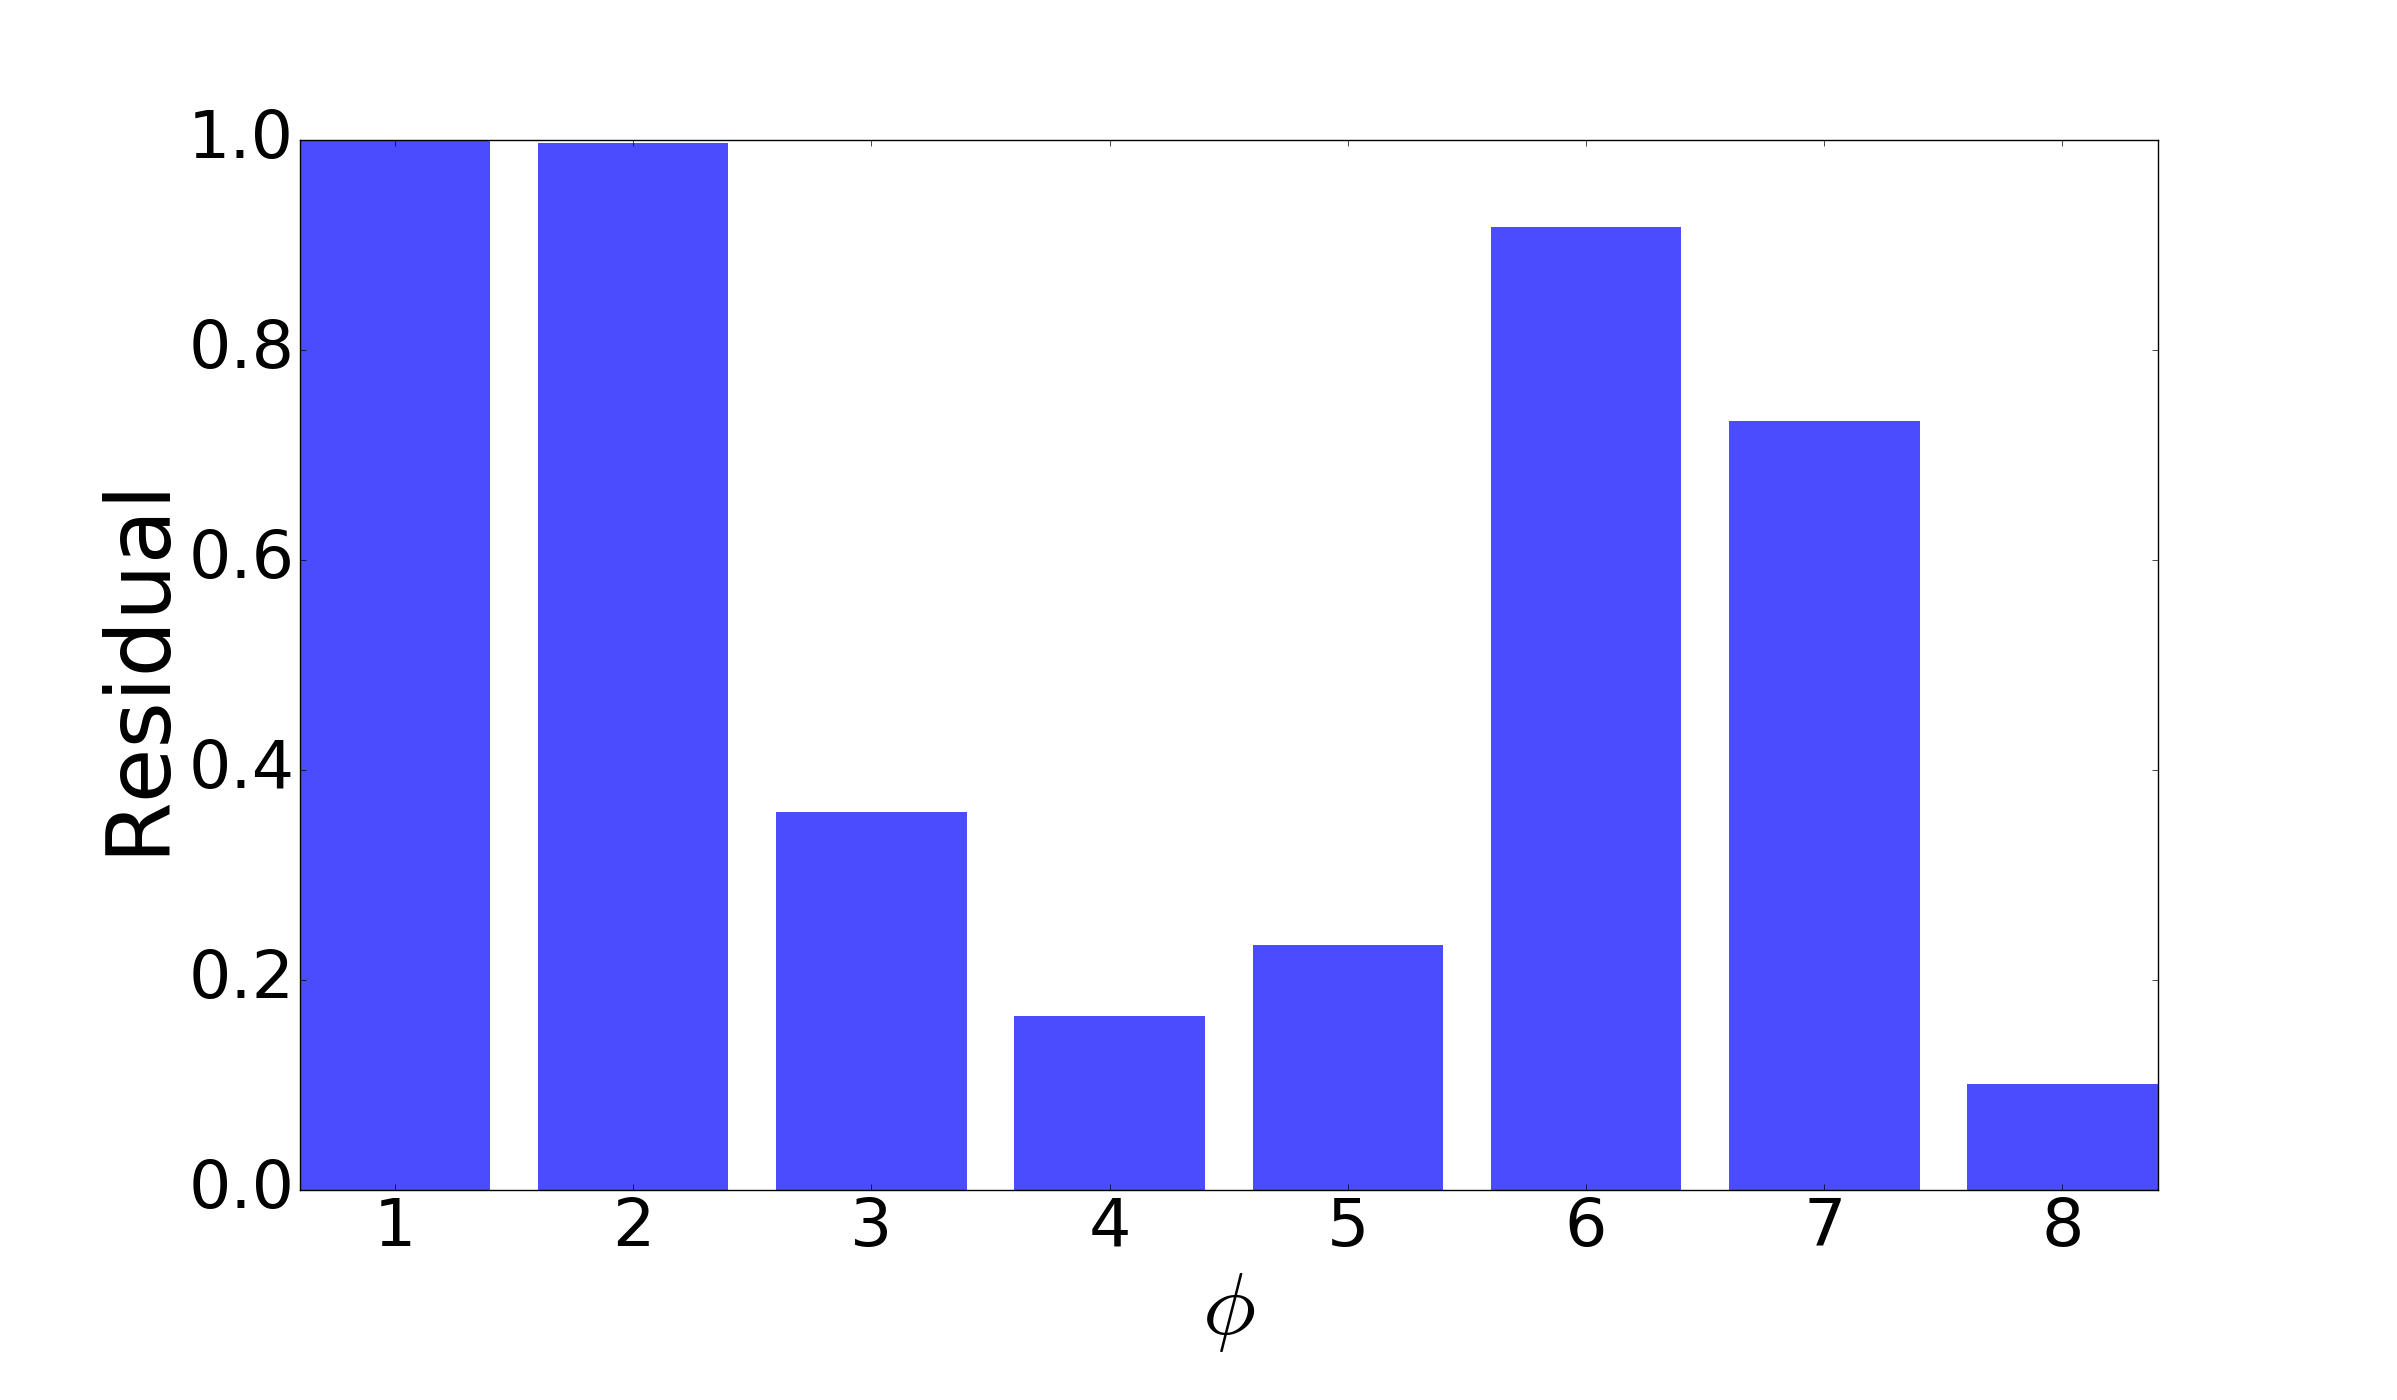
\includegraphics[width=0.6\linewidth]{residuals}
  \caption[DMAPS residuals from Michaelis-Menten system]{Residuals computed as described in previous section. High
    residuals for a given eigenvector suggest that it is not a
    function of previous eigenvectors, and thus contains new
    information. This plot suggests five significant eigenvectors, the
    first two of which parameterize significant parameter directions,
    while the final three capture sloppy
    directions. \label{fig:resids} }
\end{figure}

\section{Discussion}

The examples presented throughout this chapter show that DMAPS
consistently provides a good parameterization of the model of
interest. This parameterization is often more useful than the natural
parameter combinations originally used to formulate the system, as
DMAPS automatically accounts for regions of singular- and
regular-perturbation, in addition to detecting hidden effective
parameters. This opens the door to a number of applications, while
also inviting further research to improve certain aspects of the
method.

As we discussed in the introduction, one of the hallmarks of
sloppiness is slow convergence of model-fitting routines
\cite{transtrum_geometry_2011}. The algorithms become trapped in
sloppy regions of parameter space in which model response is nearly
constant. Thus, an obvious use of our technique would be to accelerate
these fitting procedures. The idea would be to take steps in the
DMAPS-embedding space instead of along the natural parameters. This
would require an ability to sample patches of the model manifold on
demand, and to perform extrapolation in DMAPS space. Thankfully,
results along these directions have already been established, and
these could likely be adapted to this particular setting
\cite{chiavazzo_intrinsic_2017}. We would also need the ability to map
DMAPS coordinates back to points on the model manifold. This is
related to the problem of ``lifting'' in the Equation Free framework,
again an area where existing work may be quickly incorporated
\cite{rajendran_data_2016,laing_equation-free_2015,laing_coarse-grained_2007}.

Another avenue would be nonlinear sensitivity analysis. The
simplest and most common methods simply vary individual parameters
while observing changes in model output
\cite{murphy_quantification_2004}. The shortcomings of such studies
are well known \cite{saltelli_how_2010},
but even more sophisticated methods designed for nonlinear models
assume that each parameter can be treated independently of the
others \cite{cukier_nonlinear_1978}. It would clearly be useful to
adapt this technique to the task. A simple start would be to assess
how many significant parameters a system has based on the dimension of
the DMAPS embedding \cite{dsilva_parsimonious_2015}.

Finally, further work is needed to accelerate sampling on the model
manifold. The current approach, approximate Bayesian computation, is
simple to implement but scales poorly with the dimension of parameter
space, $k$ \cite{turner_tutorial_2012}. One possibility would be to
calculate the convex hull or alpha-shape of a small sample, and then
interpolate among these points
\cite{barber_quickhull_1996,edelsbrunner_three-dimensional_1994}. Overall,
this chapter presents a novel, data-driven method to parameterize
complex models that will hopefully form the foundation for future,
practical applications.


%%% Local Variables: ***
%%% mode:latex ***
%%% TeX-master: "../../thesis.tex"  ***
%%% End: ***



% Make the bibliography single spaced
\singlespacing
\bibliographystyle{plain}

% add the Bibliography to the Table of Contents
\cleardoublepage
\ifdefined\phantomsection
  \phantomsection  % makes hyperref recognize this section properly for pdf link
\else
\fi
\addcontentsline{toc}{chapter}{Bibliography}

% % include your .bib file
% \bibliography{../references/references}

\end{document}

